%!TEX root = ../thesis.tex
%*******************************************************************************
%****************************** Third Chapter **********************************
%*******************************************************************************
\chapter{Neutron Polarization \& Transmission Measurement}
\label{ch:PT}

% **************************** Define Graphics Path **************************
\ifpdf
    \graphicspath{{figures/chapter4-figs/Raster/}{figures/chapter4-figs/PDF/}{figures/chapter4-figs/}}
\else
    \graphicspath{{figures/chapter4-figs/Vector/}{figures/chapter4-figs/}}
\fi

The nEDM@SNS experiment will employ the Magnetic Field Module (MFM), as described in \cref{ch:nEDM}, to provide the required magnetic field environment for the nEDM@SNS experiement\cite{Ahmed2019}. As shown in \cref{fig:MFM}, the nEDM MFM along with the accompanying cryostat (both of which from henceforth will be referred to as the combined cryomagnet) is made of several concentric nested vessels \cite{Ahmed2019}. As shown in \cref{fig:PT_pic}, the monochromatic polarized neutron beam will traverse the nEDM cryomagnet system from the thin metal beam windows on the outer vacuum can and the inner magnet volume, through the superconducting Pb and then through the low-cobalt high permeability Metglas before entering the central detector volume \cite{Ahmed2019}. Since the nEDM@SNS experiment requires the use of polarized neutrons, both the polarization and the transport efficiency of the neutron beam as it passes through the cryomagnet should be maximized to optimize experiment's sensitivity reach \cite{Ahmed2019}. Therefore, any mechanisms that can lead to beam polarization and beam intensity loss must be characterized and understood. This chapter describes a series of necessary polarization and transmission measurements to do so.

\afterpage{
\begin{figure}
    \centering
    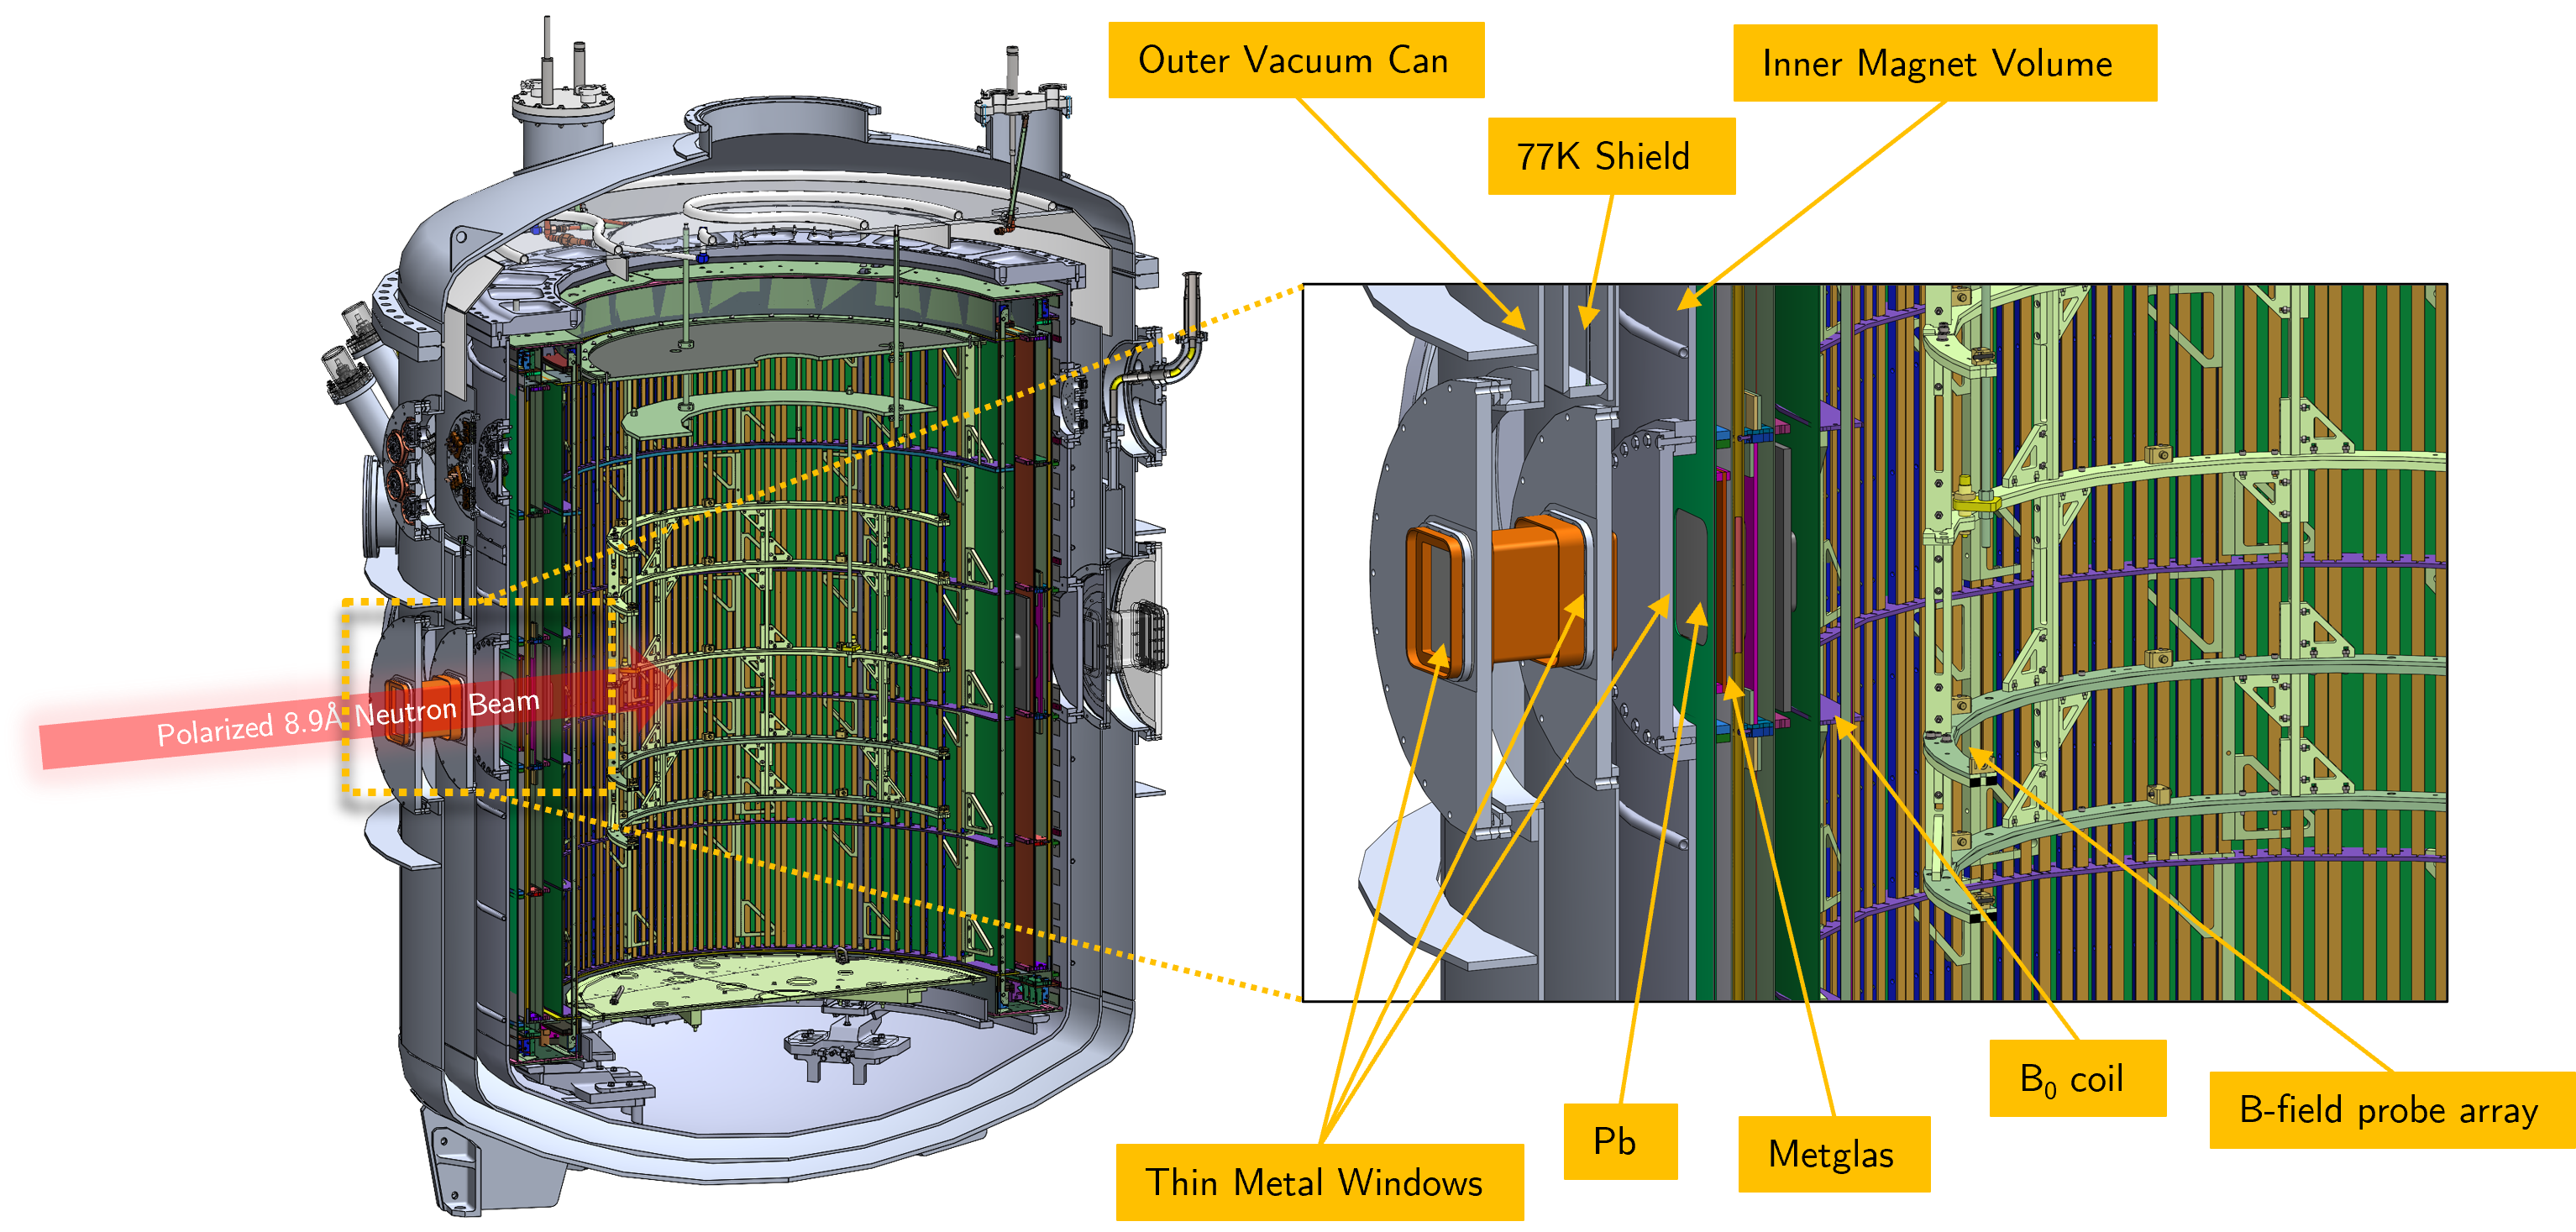
\includegraphics[width=\textwidth]{figures/chapter4-figs/PTtestpicture.png}
    \caption{Overview of proposed neutron polarization and transmission measurement for nEDM@SNS experiment at Beamline 13A. The cryomagnet shown has a vertical height of 3.6 m and a diamter of 3.05 m.}
    \label{fig:PT_pic}
\end{figure}
\clearpage}

The objective of these measurements was to determine the neutron polarization loss and transmission of each of the windows, especially Metglas, in a magnetic field environment similar to the actual nEDM experiment \cite{Ahmed2019}. The primary concern was that the presence of microscopic magnetic domains in the Metglas and the fact that both Pb and the Metglas layers can act as current sheets causing diabatic transition in magnetic field, may lead to depolarization of neutron beam \cite{Ahmed2019}. Polarization measurements through Pb samples for 4~\AA\ neutrons were performed by \cite{Treimer2012} and show strong evidence of magnetic flux trapping, but indicate a reasonable polarization transport. Furthermore, initial testing on Metglas samples were performed at SNS as well as the LENS facility at University of Indiana in 2014 and results indicated relatively minor polarization loss ($\sim$ 10\% polarization loss for 8.9~\AA\ neutrons) \cite{DEFT2014}. Even though these initial measurements indicate a small depolarization, this was attributed to the magnetic fields escaping out of the small foils from the strong applied vertical holding field these measurements were conducted in \cite{DEFT2014, Ahmed2019}. Since simulations of neutron spin orientation undergoing diabatic transition require knowledge of orientation and density of magnetic domains and surface current densities of the materials, it is difficult to determine the grain structure and current densities in Pb and Metglas foils. Therefore, the neutron polarization loss through the beam windows has to measured experimentally in the nEDM cryomagnet's geometry and magnetic field environment. 
%It should be noted that for the final nEDM@SNS experiment, the polarized $^3$He in the measurement cell can be used to recover the expected small neutron polarization loss from the cryostat magnet windows.

This chapter describes the construction of a new beamline, extending from the SNS beamline 13A, to perform the polarization and transmission experiment. Initial neutron flux characterization and dosimtery simulations will be presented. This will be followed by measurements of neutron beam polarization using the in situ polarized $^3$He spin analyzer described in \cref{ch:polHe}. Lastly, the transmission measurements of the nEDM cryomagnet neutron beam windows using small angle neutron scattering beamline at HFIR will be presented as well.

%Prior to the actual nEDM experiment, I propose here to make neutron polarization and transmission measurements at the SNS using Beamline 13A.  The objective is to determine the contribution from each of the materials that the beam passes through, especially Metglas and the superconducting  Pb, the neutron polarization loss in the magnetic field environment of the actual nEDM experiment. The applied magnetic fields and magnetic materials are shown in Fig. 2. While estimates suggest that the polarization losses should be modest it is important to confirm that the presence of magnetic domains in the actual nEDM fields and the changes in B-field between the layers do not introduce significant depolarization. In order to maintain an optimal magnetic field profile, the neutrons pass through both the Pb shield and at least one layer of the ferromagnetic flux-return made from Metglas. The magnetic properties and associated fields from these materials may lead to loss of neutron polarization and we would like to keep any losses to below a few percent. In particular there may be losses between the Pb and Metglas layers, between the Metglas and $B_0$ magnet, as well as losses in passing through the superconducting Pb and through the Metglas.



\section{Neutron Source}

%An overview of the SNS and FnPB 13 is described in detail in ref. \cite{Fomin2015}. This section is a brief recapitulation to provide context for the 2022 BL13A flux measurement and the subsequent neutron polarization and transmission measurements. 

The SNS produces neutrons via spallation by bombarding 1 GeV proton pulses onto a mercury target at a repetition rate of 60 Hz with time-averaged proton power of about 1.7 MW \cite{Fomin2015}. The high energy ($\sim$MeV) neutrons produced get moderated by a liquid hydrogen moderator down to $\sim$meV neutrons. Neutron guides are used to transport neutrons from the ports of the moderators to the individual neutron beamline instruments \cite{Fomin2015}. 

The nEDM@SNS experiment will use polarized monochromatic 8.9~\AA\ neutrons. Therefore, the polarization and transmission measurements described in this experiment will also need to be performed with polarized monochromatic 8.9~\AA\ neutrons. The SNS beamline 13 is equipped with neutron monochromators to provide such neutrons \cite{Fomin2015}. As shown in \cref{fig:BL13A}, 13A utilizes two Alkali-intercalated Graphite crystal monochromators, located 6.5 m downstream from the moderator, to select 8.9~\AA\ neutrons. The first monochromator is a type-I (lattice structure A-B-B-A) potassium intercalated graphite \cite{Mattoni2004, Courtois2011}, consisting of 24 crystals forming a mosaic, each having dimensions 20 mm x 45 mm for a total area of 120 mm x 180 mm \cite{Fomin2015}. It intersects the full beam (100 mm x 120 mm) and reflects neutrons of 8.9~\AA\ with a Bragg angle of 56$\degree$ with respect to the initial beam, as well as $\lambda$/n wavelengths with lower intensity \cite{Fomin2015}. The second monochromator is a type-I rubidium intercalated graphite crystal consisting of 35 crystals, each having dimensions 20 mm x 45 mm for a total area of 140 mm x 225 mm \cite{Fomin2015}. The second monochromator reflects the 8.9~\AA\ beam 113$\degree$ with respect to the initial beam \cite{Fomin2015}. In between the two monochromators are two graphite filters to remove the unwanted $\lambda$/n wavelength neutrons, one oriented to reflect 4.45~\AA\ ($\lambda$/2) and the other 2.97~\AA\ ($\lambda$/3) neutrons \cite{Fomin2015}. The mosaicity of the first monochromator, 3$\degree$, matches the divergence from the upstream guide and the mosaicity from the second monochromator, 5$\degree$, cancels out any first order beam divergence from the first monochromator, allowing the output beam to have the same divergence as the upstream neutron guides \cite{Mattoni2004, Courtois2011}. BL13A continues downstream after the monochromators with an 8 m expanding half ellipsoid neutron guide \cite{Fomin2015}. The beamline opens up inside the beamline 13 shielding enclosure with a rectangular opening cross section of 20 cm x 30 cm \cite{Fomin2015}.

\afterpage{
\begin{figure}
\centering
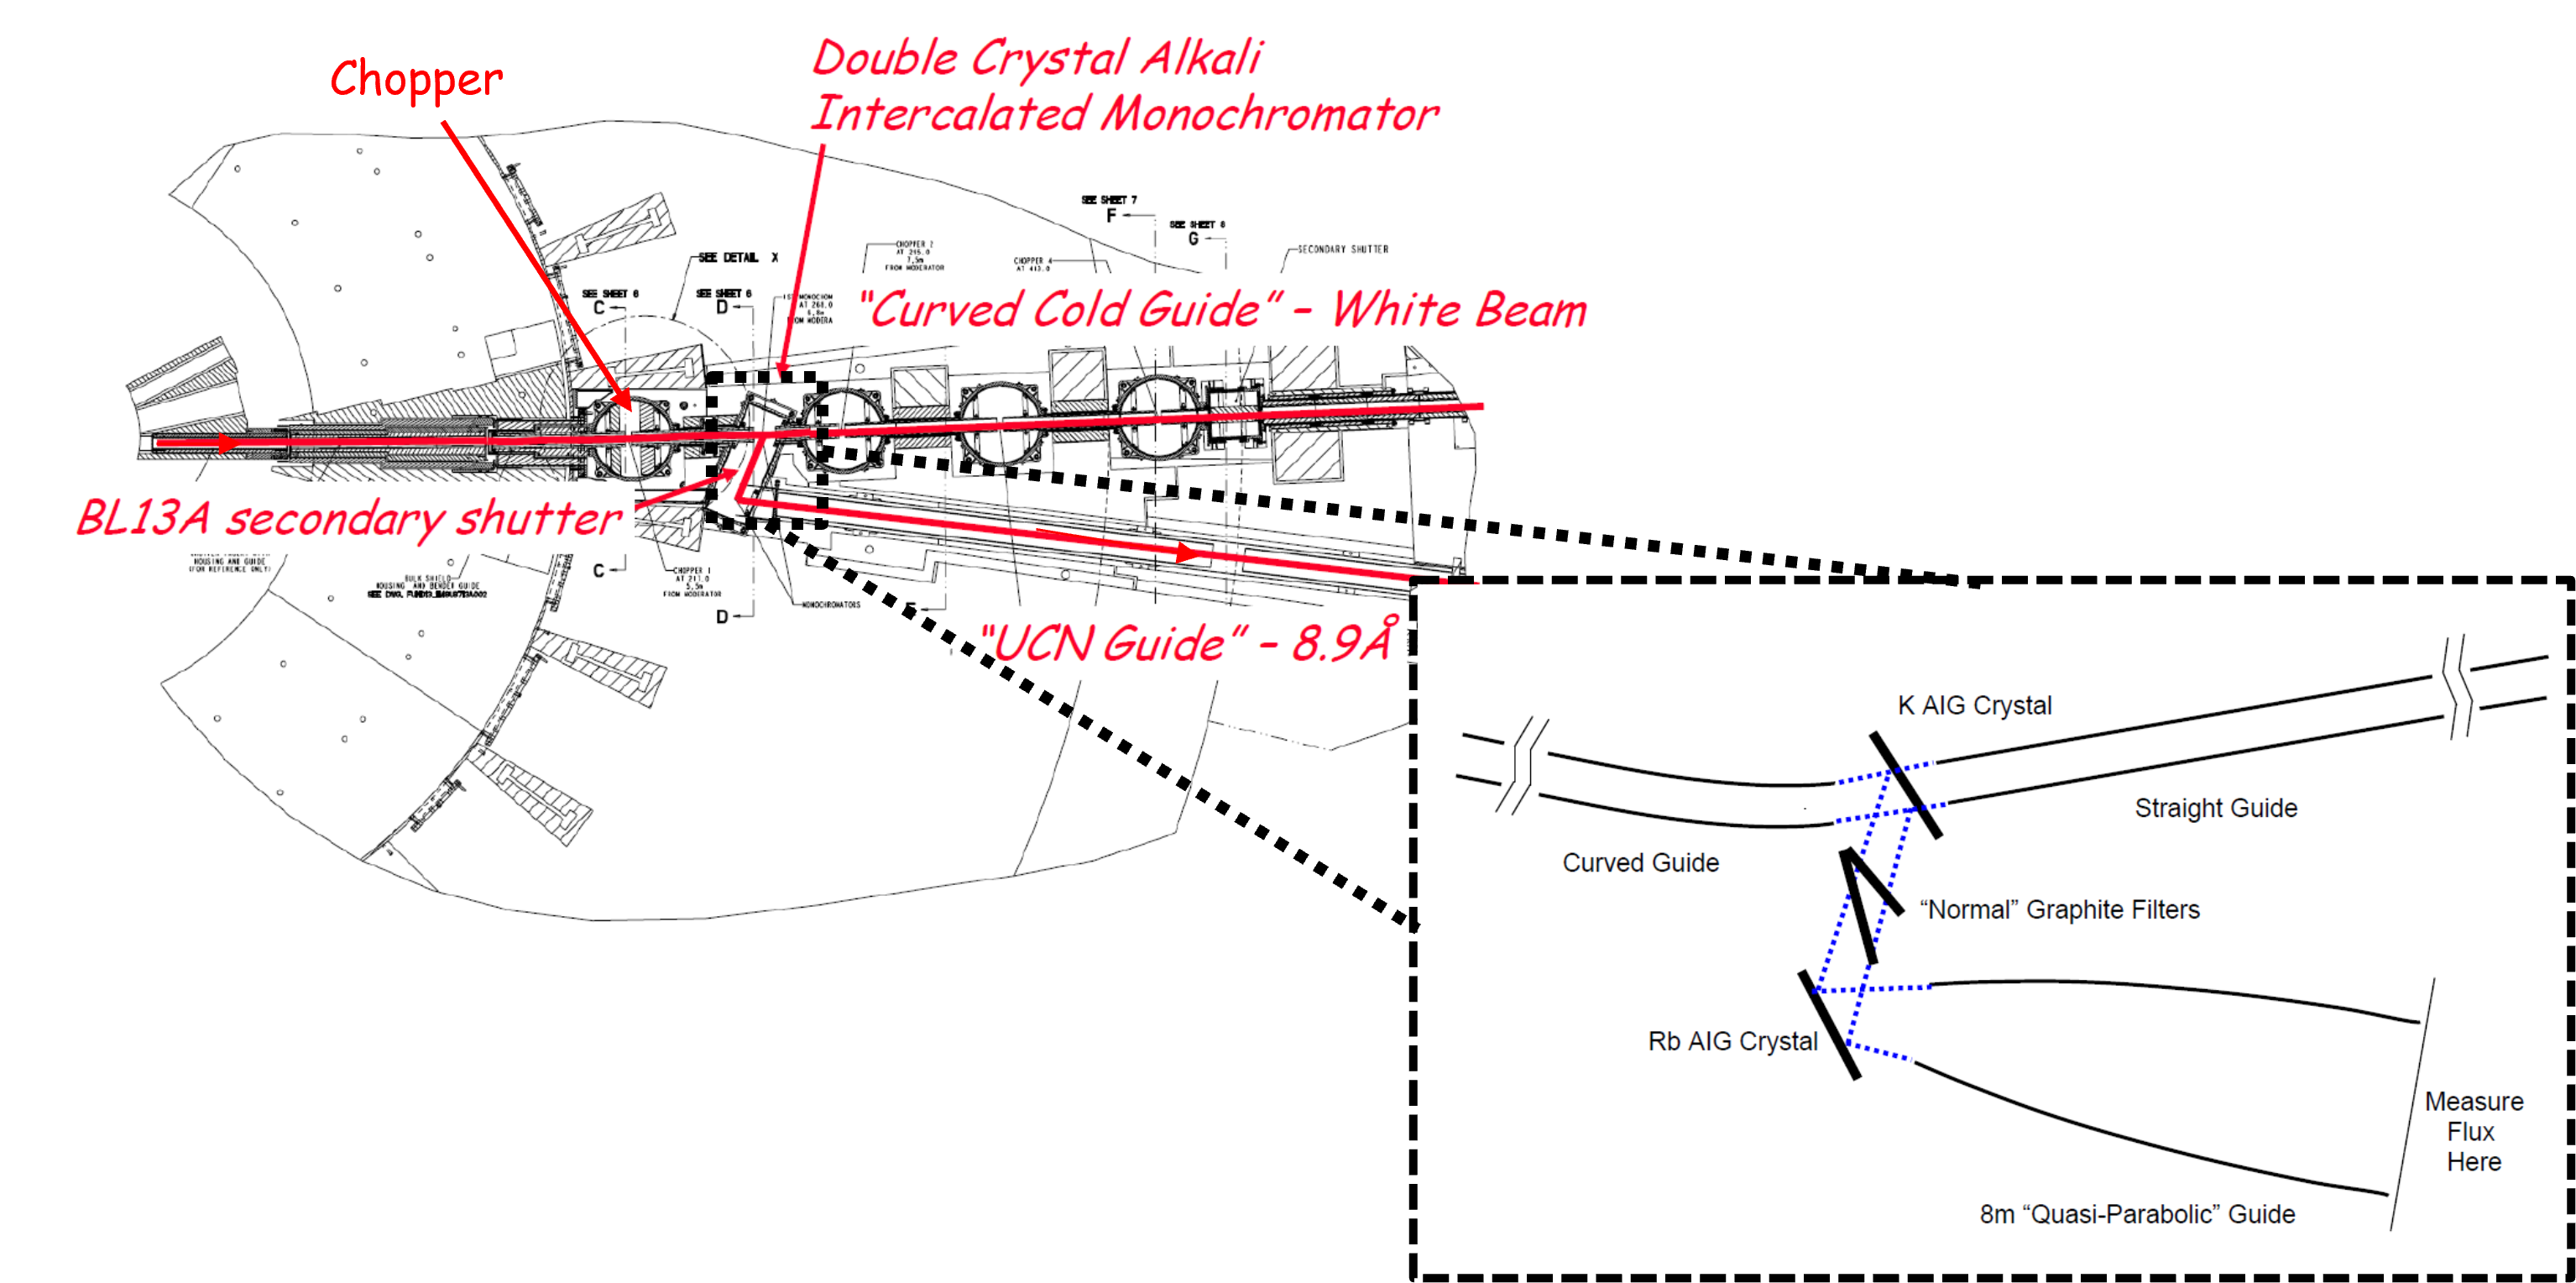
\includegraphics[width=\textwidth]{figures/chapter4-figs/BL13A_schematic.png}
\caption{A schematic diagram of the monochromatic neutron beamline 13A. The red arrows show the direction of neutron propagation. The label "UCN Guide" referes to beamline 13A.}
\label{fig:BL13A}
\end{figure}
\clearpage}

%\begin{figure}[p]
    %\centering
    %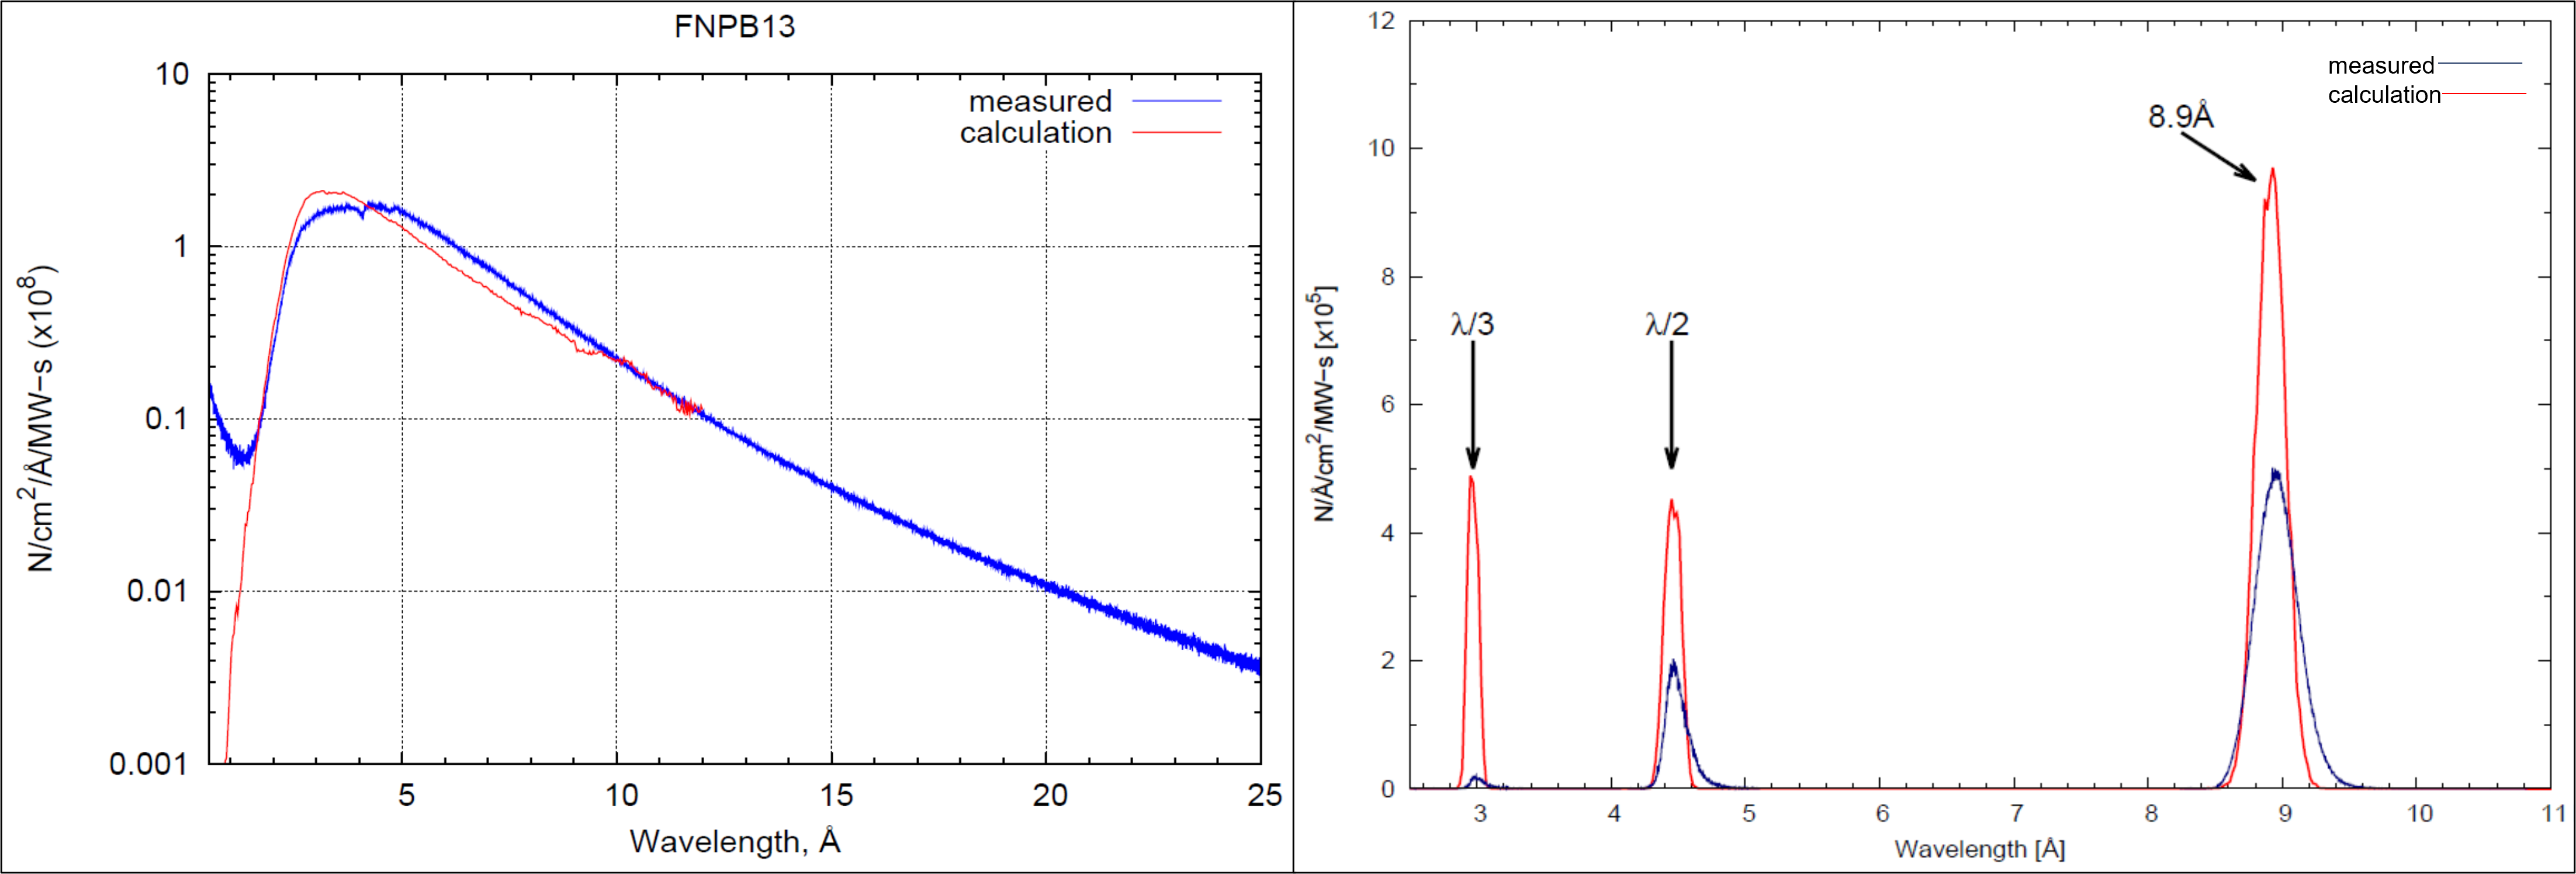
\includegraphics[width=1\textwidth, height=7cm]{beamline13flux.png}
    %\caption{Measured spectrum of neutron flux from beamline 13 (left) \cite{Fomin2015}. Measured spectrum of neutron flux from beamline 13A after the monochromator (right)\cite{Fomin2015}.}
    %\label{fig:flux}
%\end{figure}

\afterpage{
\begin{figure}[p]
    \centering
    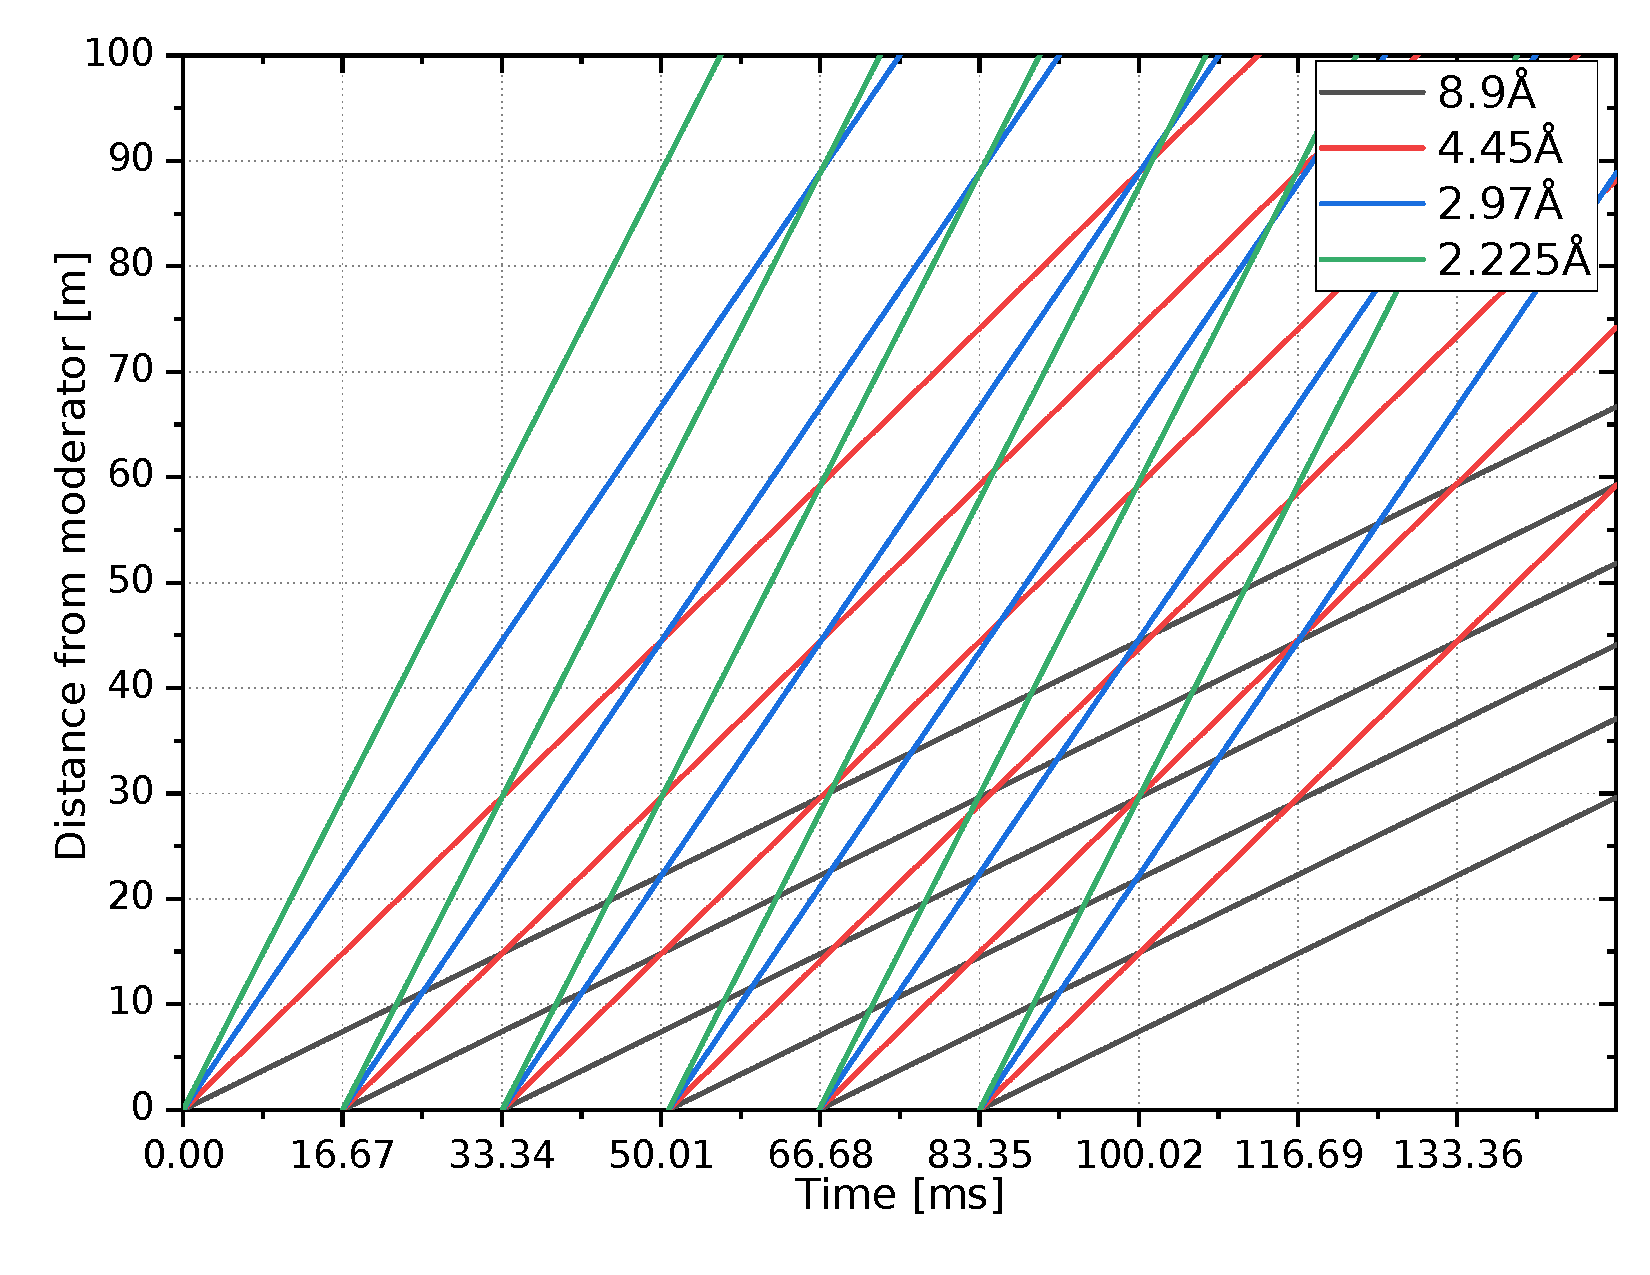
\includegraphics[width=\textwidth]{figures/chapter4-figs/frameoverlapmultipulseschedule_2.pdf}
    \caption{Multi-pulse time of flight schedule of neutrons from BL13A as the flight path of neutron increases. The curves represent velocities of 8.9~\AA, 4.45~\AA, 2.97~\AA\ and 2.225~\AA\ neutrons.}
    \label{fig:frameoverlap}
\end{figure}
\clearpage}

The SNS is a pulsed source, emitting neutrons repeatedly at 60 Hz, which allows for the determination of the neutron velocity/wavelength spectrum by measuring the neutron time of flight from the face of the moderator at fixed locations downstream of the moderator. Since there are neutrons of four discrete velocities coming from beamline 13A (444.5 m/s, 888.9 m/s, 1333.9 m/s and 1778 m/s corresponding to 8.9~\AA, 4.45~\AA, 2.97~\AA\ and 2.225~\AA\ respectively), there is possibility of frame overlap of neutrons i.e. 888.9 m/s and 1333.9 m/s neutrons from different pulse frames overlapping with the arrival time of 444.5 m/s neutrons at distances downstream of the moderator. \Cref{fig:frameoverlap} illustrates this effect for BL13A. Frame overlap choppers can be used to isolate desired wavelength of neutrons. These choppers are rotating disks made of neutron-absorbing material with a "pizza-slice" shape cut out. If these choppers are placed at a distance from the moderator and their rotation is phased to the neutron pulse frequency (for e.g. 60Hz), then only neutrons of a particular wavelength (those that arrive when the "pizza-slice" cut is aligned with the beam) will be transmitted. BL13A has one frame overlap chopper at 5.5m from the face of the moderator.

The chopper has an opening angle of $131\degree$ so $ \frac{131\degree}{360\degree} \times \frac{1}{60~\text{Hz}} = 6.06$ ms. This is the the full acceptance width of chopper1 in time of flight. With the chopper opening is 180\degree offset from the guide, the 6.06 ms acceptance window is centered at 8.333 ms, half the time of the 16.67 ms frame. This acceptance will allow neutrons of arrival time within the range of 5.3 ms (8.33 ms-$\frac{6.06 \text{ms}}{2}$) to 11.36 ms (8.333 ms+$\frac{6.06\text{ms}}{2}$). At 5.5m, the arrival times of 2.225~\AA\ (1777 m/s), 2.97~\AA\ (1331 m/s) and 4.45~\AA\ (888 m/s) neutron are 3.1 ms, 4.13 ms and 6.19 ms, respectively. The 2.225~\AA\ (3.1 ms) and 2.97~\AA\ (4.13 ms) miss the acceptance window since 3.1 ms and 4.13 ms are less than 5.3 ms but the 4.45~\AA\ do not, 6.19 ms is greater than 5.3 ms. A time of flight delay needs to be applied, so the chopper can block out the 4.45~\AA\ neutrons, otherwise, they will cause a frame overlap with 8.9~\AA\ neutrons as the flight path of neutron increases. This is shown in \cref{fig:frameoverlap}. With the delay of 5.3 ms, to the no delay center of acceptance of 8.333 ms, the new center of acceptance is at 13.63 ms and the leading edge becomes 10.60 ms(13.63 ms-$\frac{6.06\text{ms}}{2}$) and the lagging edge becomes 16.67 ms (13.63 ms+$\frac{6.06\text{ms}}{2}$) and the 4.45~\AA\ get blocked by the chopper. Now, all of wavelength orders will miss the acceptance set by chopper with a 5.3 ms phase delay, except 8.9~\AA. \Cref{fig:single_pulse_ts_9ang} shows the time of flight pulse schedule with the chopper delay of 5.3 ms and the subsequent wavelength acceptance band of only 8.9~\AA, shown in \cref{fig:trans_9ang}. The reason why the delayed acceptance center is set at 13.36 ms is partly historical as well. The flux characterization measurement of BL-13A in 2010, prior to proposal of this experiment, used a delay of 5.3 ms. The time of flight sequence described above was used to define the full 16.67 ms time of flight frames for the 8.9~\AA\ neutrons, as shown in \cref{fig:multi_pulse_ts_9ang}, for the subsequent measurements.  


\afterpage{
\begin{figure}[p]
    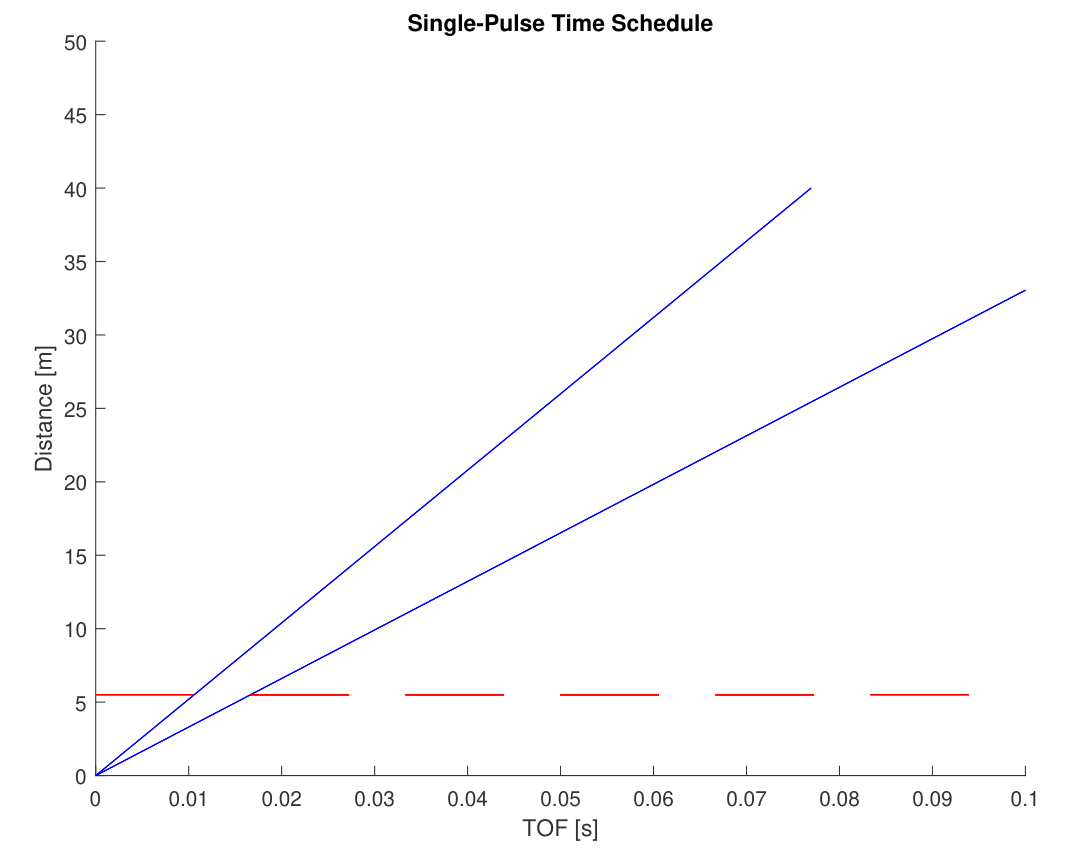
\includegraphics[width=\textwidth]{figures/chapter4-figs/chop_1_single_pulse_ts_9ang.png}
    \caption{Simulated single neutron pulse time of flight schedule for chopper set to 5.3 ms delay to transmit 8.9~\AA\ neutrons. The chopper acceptance is shown in red and the neutron velocity acceptance is shown in blue.}
    \label{fig:single_pulse_ts_9ang}
 \end{figure}
\clearpage}

\afterpage{
\begin{figure}[p]
    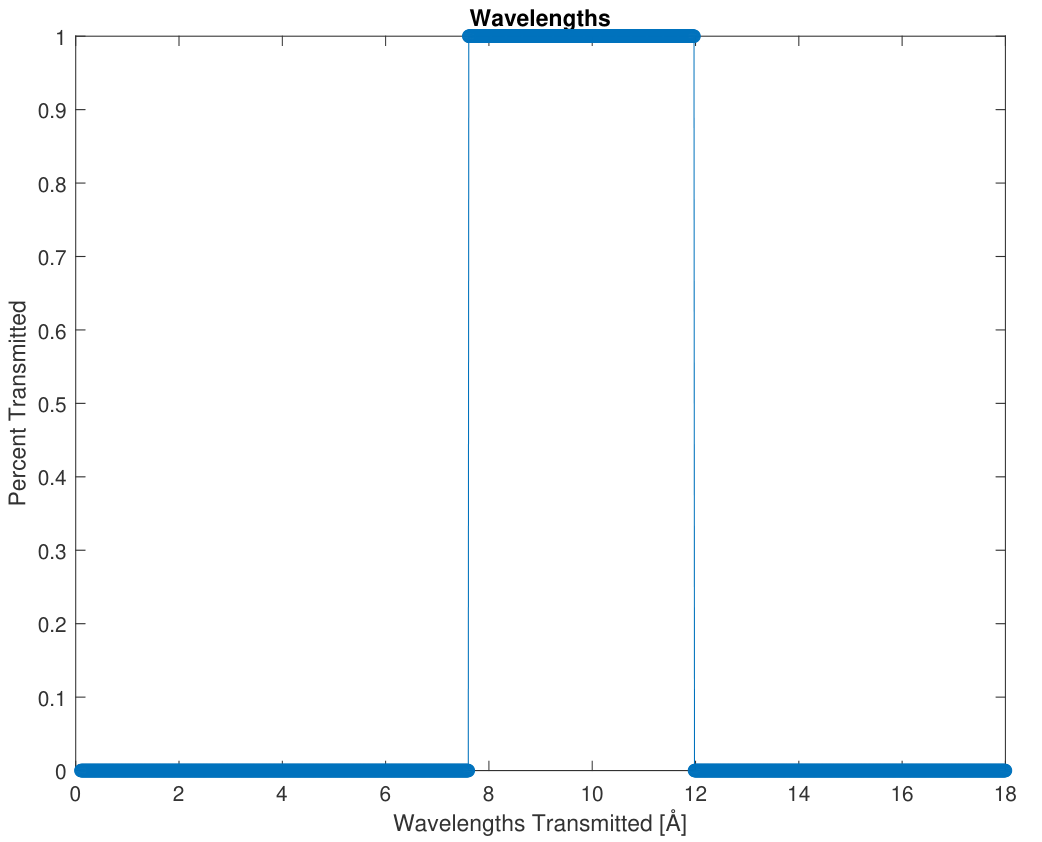
\includegraphics[width=\textwidth]{figures/chapter4-figs/chop_1_transmission_9ang.png}
    \caption{Simulated neutron transmission spectrum for chopper set to 5.3 ms delay.}
    \label{fig:trans_9ang}
\end{figure}
\clearpage}

\afterpage{
\begin{figure}[p]
    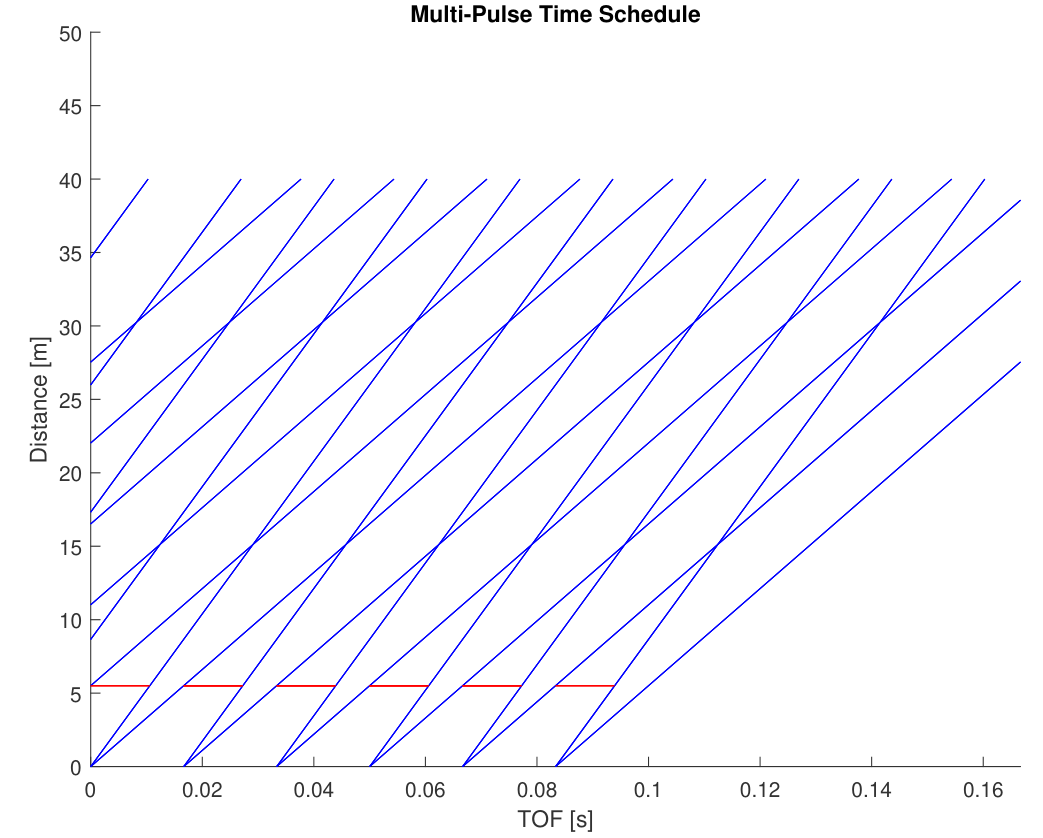
\includegraphics[width=\textwidth]{figures/chapter4-figs/chop_3_multi_pulse_ts_9ang.png}
    \caption{Simulated multiple neutron pulse time of flight schedule for chopper set to 5.3 ms delay to transmit 8.9~\AA\ neutrons. The chopper acceptance is shown in red and the neutron velocity acceptance is shown in blue.}
    \label{fig:multi_pulse_ts_9ang}
\end{figure}
\clearpage}

\subsection{Beamline 13A Flux Measurement}
   
Prior to the polarization and transmission measurements, the initial neutron flux from the currently existing 13A neutron guide was measured to verify the operation of the monochromators. The previous 13A flux measurement was performed in 2010 \cite{Fomin2015}, therefore, it was crucial to once again verify the health of the monochromators before the polarization and transmission measurement was commenced in 2022. Any decrease in neutron flux will indicate possible degradation of the monochromator's performance and/or any of the beamline neutron guides. %A beam flux reduction to within $10\%$ of the 2010 flux would allow the continuation of the polarization and transmission measurement without a significant negative effect on the measurement's statistical sensitivity. 
This section reports on the 13A flux measurement performed in June 2022. The measurement setup, the results and their implication for the polarization and transmission measurement are discussed.

\subsubsection{Measurement Setup}

A calibrated n-$^3$He low efficiency proportional detector (LND 2232/NIM) was mounted on Al-80/20 support stand and placed after a 1 cm Lithium aperture on the guide exit, giving a total neutron flight distance of 16.04 m from the face of the moderator to the detector. The detector pulse height spectrum was calibrated with a 20 mCi $^{252}$Cf source prior to the measurement. The output from the detector was fed into a pre-amplifier. Both the detector and the pre-amplifier were powered using a NIM crate. The detector had an operating voltage of 800 V. The existing BL13A guide had a 2 inch neutron beam window in front of the 30 cm x 20 cm guide terminal. A lithium aperture with an opening area of 4.28 cm$^2$ was installed on the guide window. This was done to prevent saturating the neutron detector with a high count rate.

\afterpage{
\begin{figure}
\centering
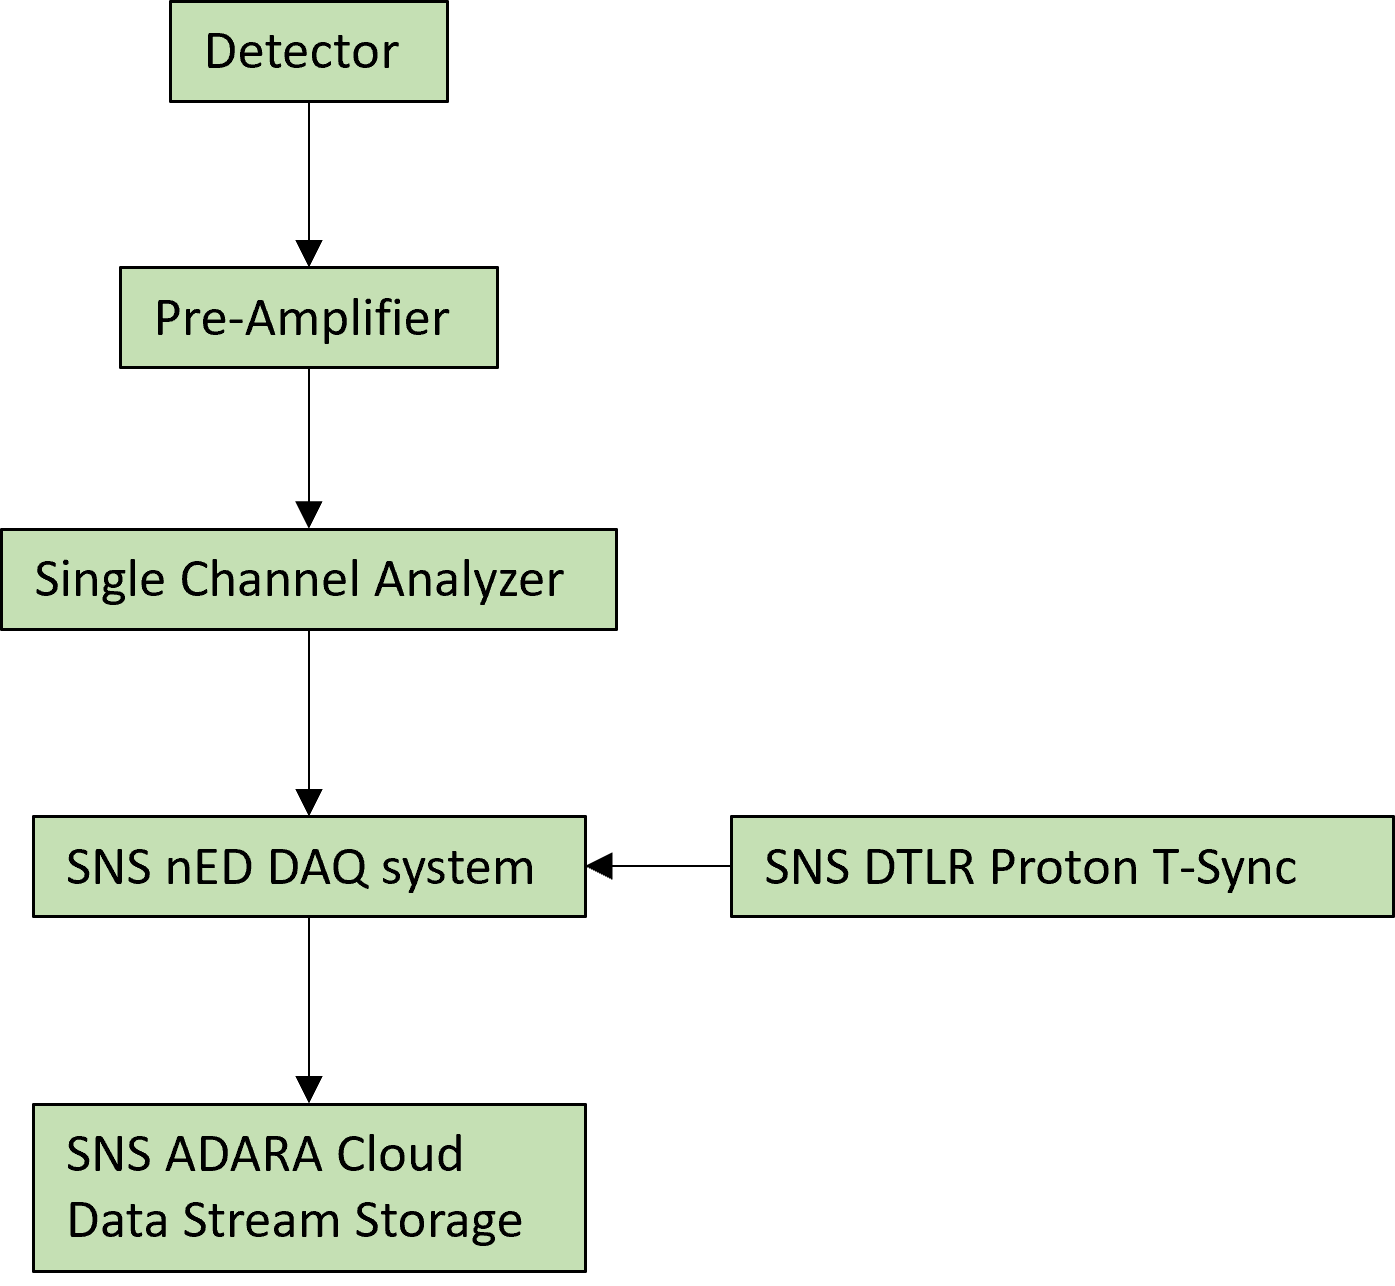
\includegraphics[width=0.5\textwidth]{figures/chapter4-figs/P1_DAQ_Diagram.png}
\caption{Data acquisition setup for June 2022 13A Flux Measurement}
\label{fig:flux_DAQ}
\end{figure}
\clearpage}

The data collection flowchart is shown in \cref{fig:flux_DAQ}. The output from the pre-amplifier was fed into a Single Channel Analyzer (SCA). The SCA had a lower level (LL) of 2 V and a window of 2 V. If the signal from pre-amp fell within the window set between the LL and UL, then the SCA would discriminate on the pre-amplifier analog output and produce a TTL pulse to be sent to the SNS Neutron Event Distributor (nED) DAQ for counting. nED DAQ system was also taking the Real Time Data Link (RTDL) proton beam T$_0$ trigger signal (Event 39) to time synchronize the logic pulses coming from the SCA. The nED DAQ system packed the data into HDF5 data structures and uploaded it to the cloud stream for data analysis.

To start the measurement, the monochromator was lowered into the beam path at the nominal position. This was done via the BL13 FIDO motor control box, which operates the stepper motors that control the crystal's motional degrees of freedom. Only the first linear motor, which vertically translates the monochromator into the beam path, was utilized. There are motors which control the crystal's tilt and rotational degree of freedom but those were kept at their previously optimized settings.

\subsubsection{Analysis and Results}

As shown in \cref{fig:frameoverlap}, there is frame overlap present from $\lambda$ and $\lambda/2$ neutrons at the location of the detector (16.04 m). BL-13A chopper was utilized in this flux measurement to prevent frame overlap. \Cref{fig:chopp_open} shows the time of flight spectrum with the chopper parked at the fully open position. The figure shows the four neutron wavelengths harmonics at the detector location according to their expected time of flight per frame with 100 $\mu$s time bin. The multi-pulse schedule in \cref{fig:frameoverlap} shows that at the detector location, the 8.9~\AA\ and 4.45~\AA, have approximately same arrival time. As shown in \cref{fig:chopp_open}, the dominant peak around 3000 $\mu$s is the 8.9~\AA\ peak and the visible shoulder, around 2000 $\mu$s is the frame overlapping 4.45~\AA\ peak. The peak at around 12000 $\mu$s is the 2.97~\AA\ peak and the low intensity peak at around 8000$\mu$s is the 2.225~\AA\ peak. To separate out the 8.9~\AA\ neutrons from the 4.45~\AA\ neutrons, the chopper was operated at the 5.3 ms phased time delay. \Cref{fig:5.3ms} shows the isolation of the 8.9~\AA\ neutrons from the higher orders with a chopper delay of 5300 $\mu$s and \cref{fig:12.8ms} shows the isolation of the higher orders with a chopper delay of 12800 $\mu$s. The time of flight spectrum in \cref{fig:chopp_run} was analysed to obtain a neutron flux spectrum as a function of wavelength. To do this, first step was to add the 16667$\mu$s frames to the wavelength orders according to their arrival time, as shown in \cref{fig:frameadd}, to obtain an absolute time of flight spectrum. The 8.9~\AA\ neutrons arrive in the third frame, therefore, 33334 $\mu$s (two frames after T$_0$) were added to their arrival time. The 4.45~\AA\ neutrons arrive in the second frame, therefore, 16667 $\mu$s (one frame after T$_0$) were added to their arrival time. The 2.97~\AA\ and 2.225~\AA\ arrive in the first frame.

\afterpage{
\begin{figure}
\centering
  \begin{subfigure}[b]{0.49\textwidth}
    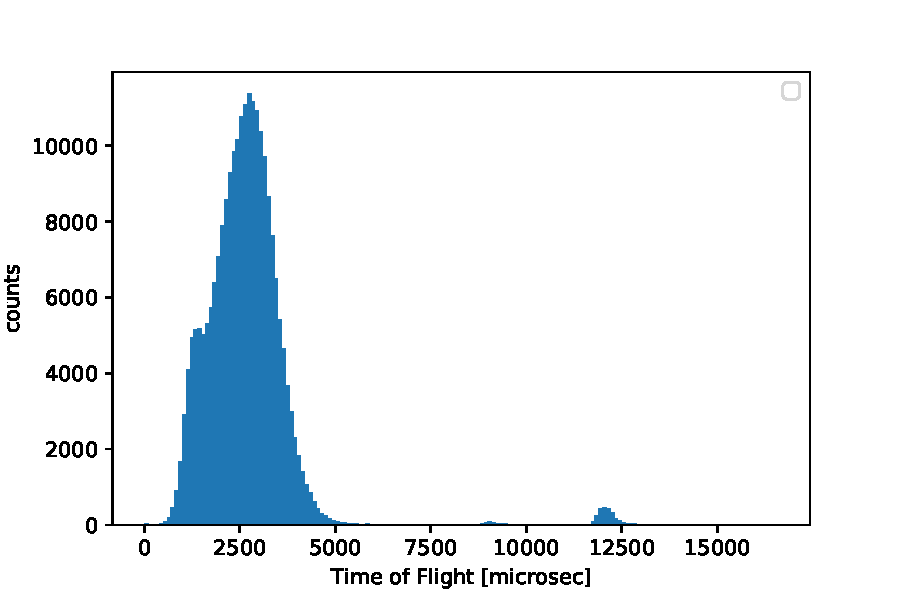
\includegraphics[width=\textwidth]{13A_Chopp_open.pdf}
    \caption{linear-linear axis}
    \label{fig:linlin}
  \end{subfigure}
  \hfill
  \begin{subfigure}[b]{0.49\textwidth}
    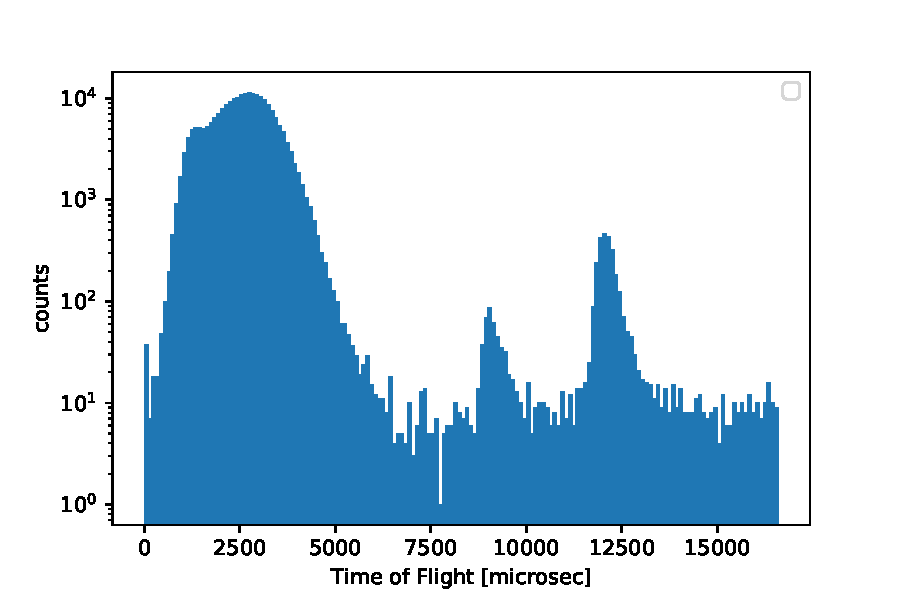
\includegraphics[width=\textwidth]{13A_Chopp_open_log.pdf}
    \caption{log-linear axis}
    \label{fig:loglin}
  \end{subfigure}
  \caption{13A time of flight spectrum with chopper fully parked open.}
  \label{fig:chopp_open}
\end{figure}

\begin{figure}
\centering
  \begin{subfigure}[b]{0.49\textwidth}
    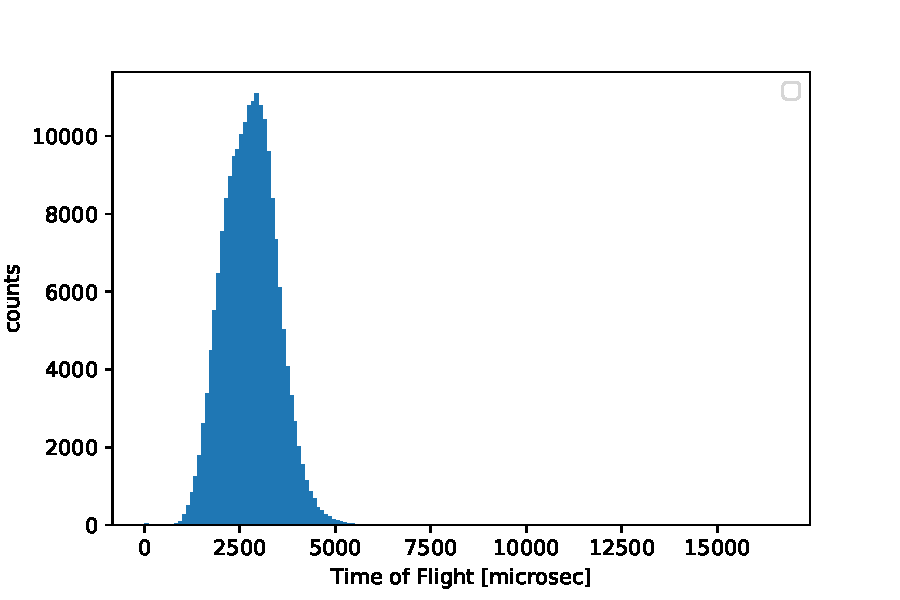
\includegraphics[width=\textwidth]{13A_5300microsec__neg25mm_300s.pdf}
    \caption{Chopper phase delay of 5.3 ms to isolate the $\lambda$ neutrons.}
    \label{fig:5.3ms}
  \end{subfigure}
  \hfill
  \begin{subfigure}[b]{0.49\textwidth}
    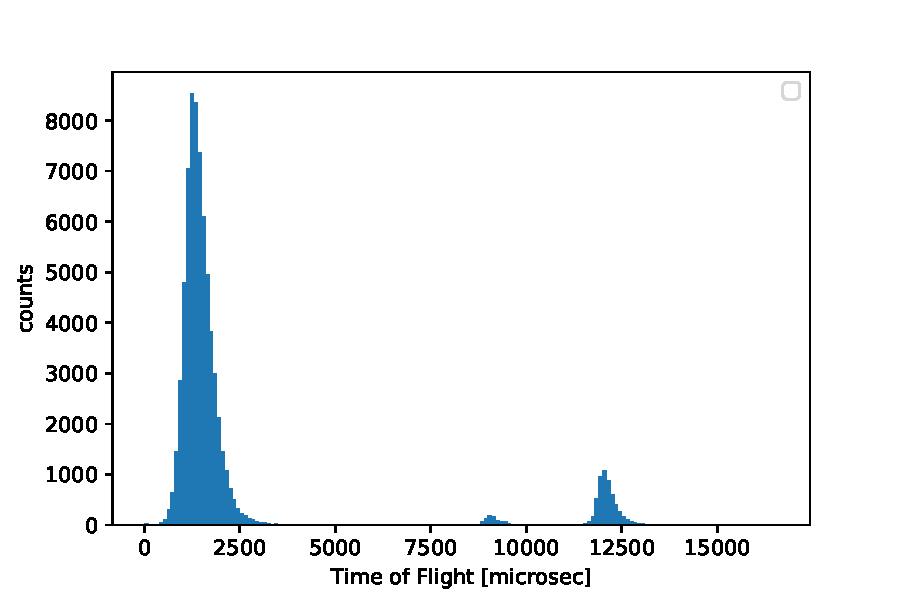
\includegraphics[width=\textwidth]{13A_12800_695.pdf}
    \caption{Chopper phase delay of 12.8 ms to isolate the $\lambda/2$, $\lambda/3$ and $\lambda/4$ neutrons.}
    \label{fig:12.8ms}
  \end{subfigure}
  \caption{13A time of flight spectrum with chopper running at select phases to isolate the first order peak from the higher orders.}
  \label{fig:chopp_run}
\end{figure}

\begin{figure}
\centering
  \begin{subfigure}[b]{0.49\textwidth}
    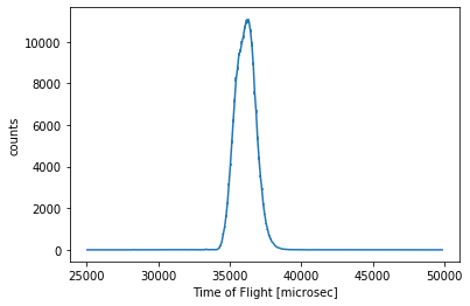
\includegraphics[width=\textwidth]{chop_frameadd_2.png}
    \caption{33334 $\mu$s added (two frames after T$_0$) for $\lambda$ neutrons}
    \label{fig:frame2}
  \end{subfigure}
  \hfill
  \begin{subfigure}[b]{0.49\textwidth}
    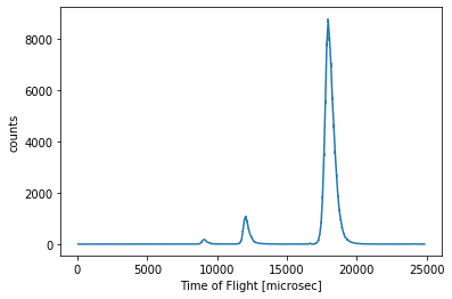
\includegraphics[width=\textwidth]{chop_frameadd_1.png}
    \caption{16667 $\mu$s added (one frame after T$_0$) for $\lambda/2$ neutrons.}
    \label{fig:frame1}
  \end{subfigure}
  \caption{13A time of flight spectrum with addition of the respective 60Hz frames to get the absolute time of flight in bin width of 100 $\mu$sec.}
  \label{fig:frameadd}
\end{figure}
\clearpage}

The neutron time of flight was converted to neutron wavelength using the relation:
\begin{equation}
    \lambda = \frac{h}{m_n}\frac{t}{L}
\end{equation}
where $\lambda$ is the neutron's wavelength in m, $h$ is the Planck's constant, $m_n$ is the neutron's mass in kg, $t$ is the neutron's time of flight in seconds and $L$ is the neutron's flight distance from the moderator to the detector in meters. This is shown in \cref{fig:framewave}. Prior to the measurement, the efficiency of the neutron detector was measured to be $7.5\times10^{-5} \frac{\text{counts}}{\text{neutrons}}$ at 1~\AA. This efficiency scales linearly with the reciprocal of the neutron velocity at longer neutron wavelengths. This efficiency plus the area of the aperture, 4.28 cm$^2$, were used to convert the histogram in  \cref{fig:neutroneff} from counts per time bin to neutrons per cm$^2$ per time bin in \cref{fig:neutronbinwidth}. The normalization with respect to proton power was done to take into account any accelerator power drop or any proton pulse drops. The charge per proton pulse is measured by the SNS and included in the instrument data acquisition for normalization of neutron flux to the total or per pulse incident protons \cite{Blokland2006}. Given the energy of the pulsed proton beam is 1 GeV, the proton charge was converted to beam power as:
\begin{equation}
    \text{Proton Charge [pC]} \times \frac{1\text{[C]}}{1\times10^{12} \text{[pC]}} \times  \frac{1000.0 \text{[MeV]}}{1 e} \times \frac{1 \text{[J]}}{1 \text{[C $\cdot$ V]}} \times \frac{1 \text{[MW $\cdot$ sec]}}{1 \text{[MJ]}} 
\end{equation}
From this, \cref{fig:neutronbinwidth} was normalized to obtain \cref{fig:neutronpower}, the neutron spectrum per any proton beam power. The neutron flux spectrum as a function of wavelength from 2010 and 2022 measurements is shown in \cref{fig:flux_wavelength}.

\afterpage{
\begin{figure}
    \centering
        \begin{subfigure}[b]{0.475\textwidth}
            \centering
            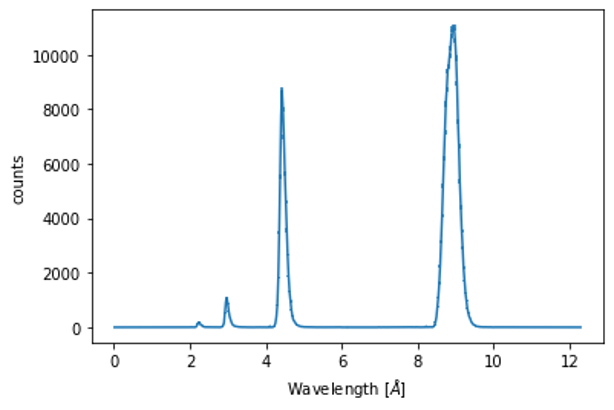
\includegraphics[width=\textwidth]{chop_stitch.png}
            \caption{13A spectrum normalized to efficiency of neutron detector as well as the area of aperture.}    
            \label{fig:framewave}
        \end{subfigure}
        \hfill
        \begin{subfigure}[b]{0.475\textwidth}  
            \centering 
            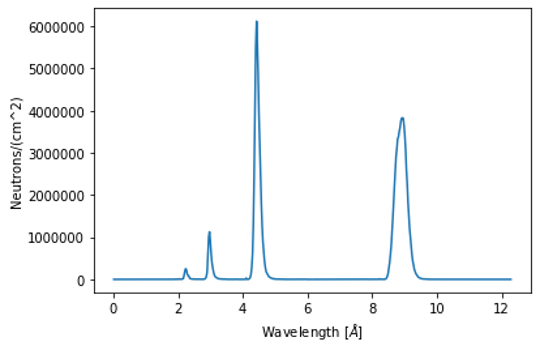
\includegraphics[width=\textwidth]{chop_eff_area.png}
            \caption{13A spectrum normalized to efficiency of neutron detector as well as the area of aperture.}   
            \label{fig:neutroneff}
        \end{subfigure}
        \vskip\baselineskip
        \begin{subfigure}[b]{0.475\textwidth}   
            \centering 
            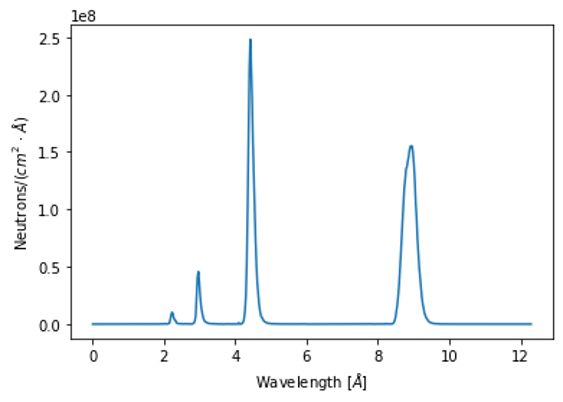
\includegraphics[width=\textwidth]{chop_bin.png}
            \caption{13A spectrum normalized to wavelength bin width.}    
            \label{fig:neutronbinwidth}
        \end{subfigure}
        \hfill
        \begin{subfigure}[b]{0.475\textwidth}   
            \centering 
            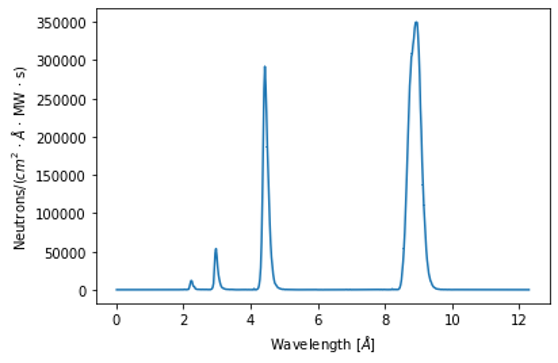
\includegraphics[width=\textwidth]{chop_power.png}
            \caption{13A spectrum normalized to the SNS proton beam power.}    
            \label{fig:neutronpower}
        \end{subfigure}

\caption{Normalization procedures for analysis of the BL-13A neutron flux measurement.} 
\label{fig:Fluxanalysis}
\end{figure}
\clearpage}

\afterpage{
\begin{figure}
\centering
  \begin{subfigure}[b]{\textwidth}
    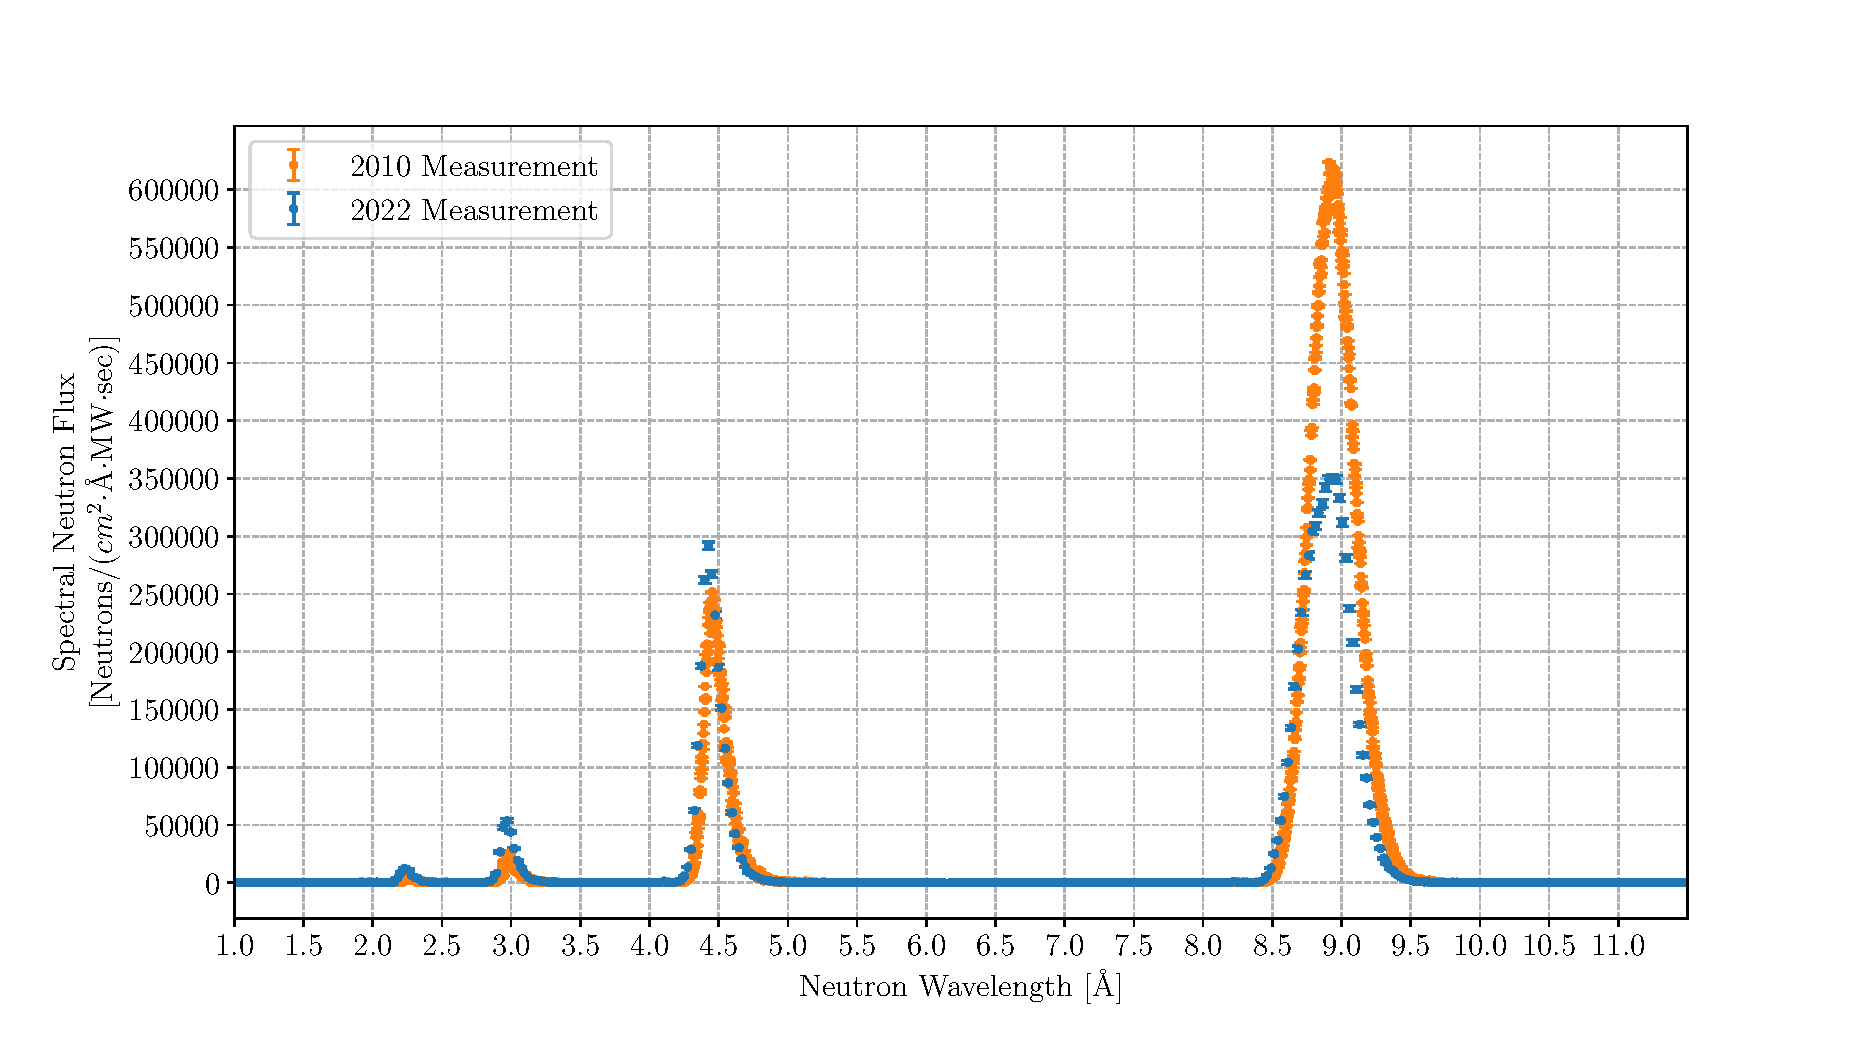
\includegraphics[width=\textwidth]{SpectralNeutronFlux_2010_2022_linlin.pdf}
    \caption{linear-linear axis}
    \label{fig:linlin}
  \end{subfigure}
  \hfill
  \begin{subfigure}[b]{\textwidth}
    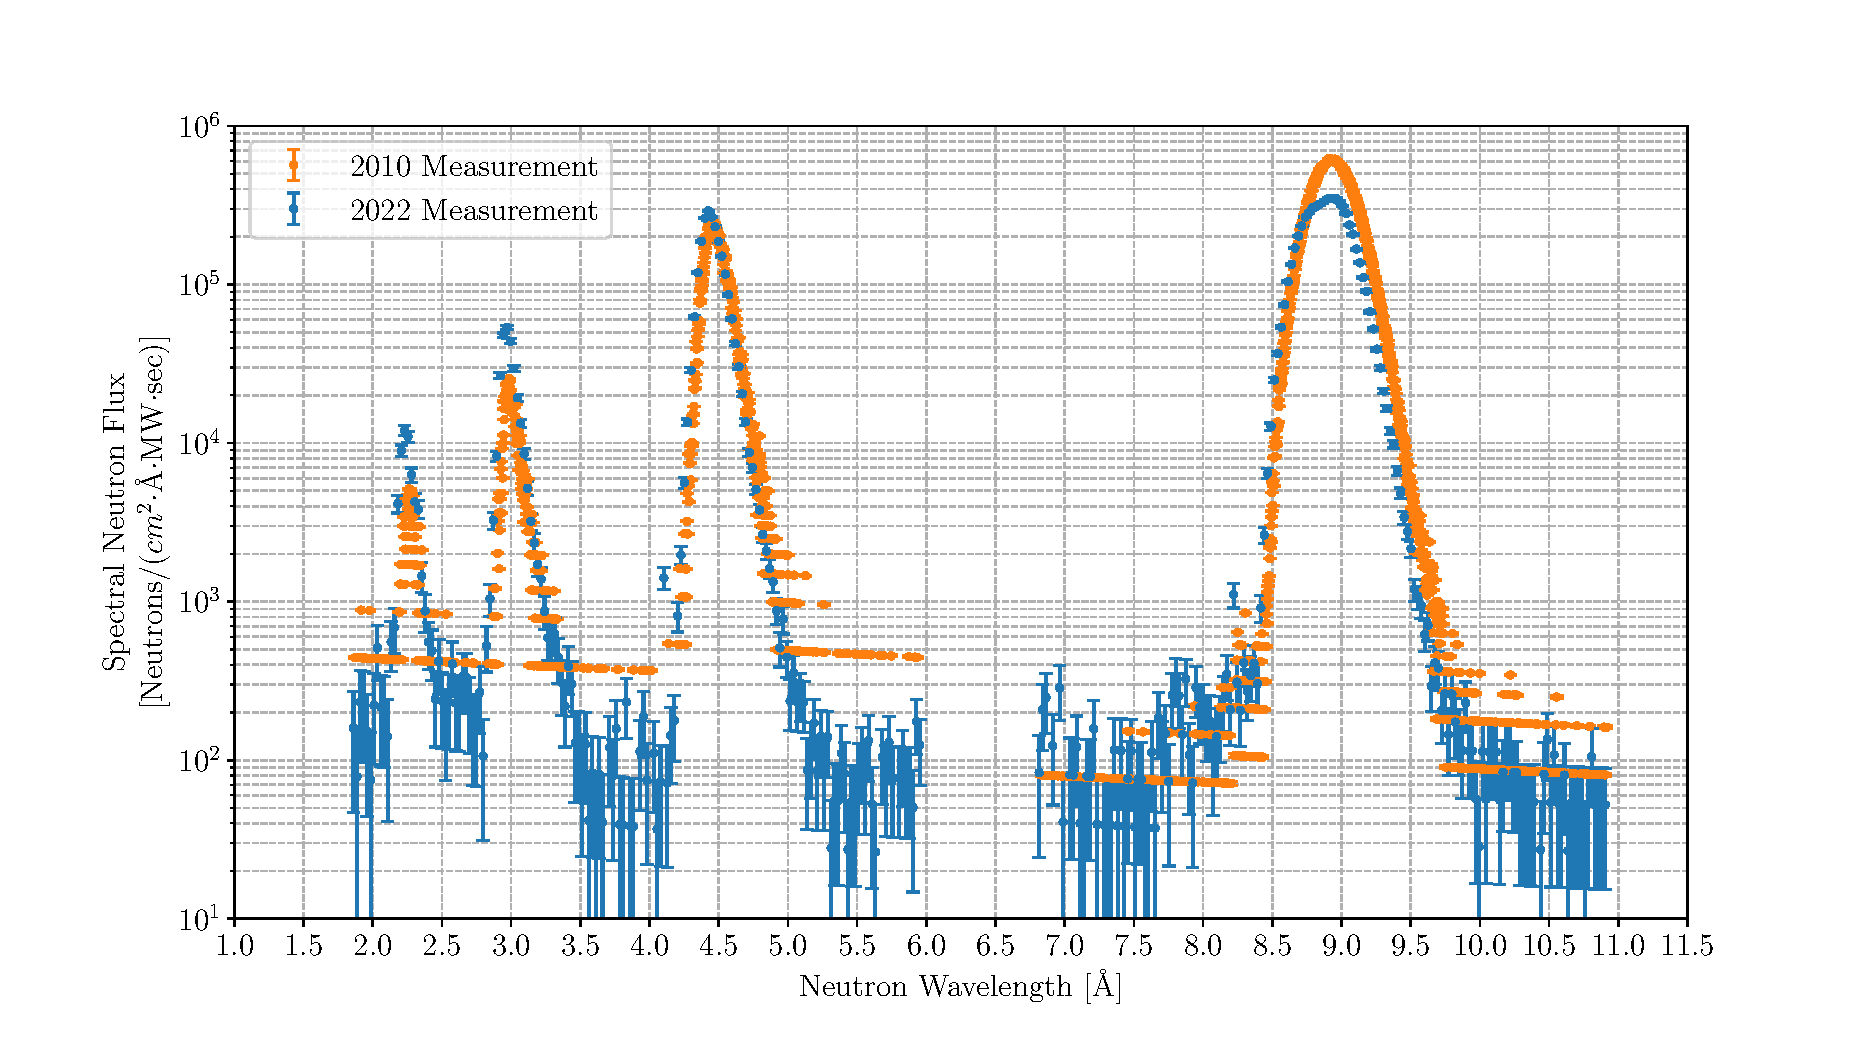
\includegraphics[width=\textwidth]{SpectralNeutronFlux_2010_2022_loglin.pdf}
    \caption{log-linear axis}
    \label{fig:loglin}
  \end{subfigure}
  \caption{Measured 13A Flux spectrum as a function of neutron wavelength.}
  \label{fig:flux_wavelength}
\end{figure}
\clearpage}

\subsubsection{Discussion}

\Cref{fig:flux_wavelength} shows that the 13A monochromator is reflecting the same wavelength of neutrons in 2022 as it did in 2010. The exception arises when one compares the peak intensity for the four neutron wavelength orders. The 8.9~\AA\ neutrons, have a lower peak intensity in 2022 from 2010 while the higher order neutrons are showing a high peak intensity in the 2022 measurement as compared to 2010 measurement. This change in intensity for 2022 flux in the different orders of neutron wavelengths can be caused by monochromator crystal orientation misalignment or degradation of the monochromator crystal lattice intercalation spacing or the change in the moderator spectrum as compared to 2010.

Previous measurements with the (LND 2232/NIM) were used to look at the instantaneous count rate for dead time. They indicated minimal dead time at better than 30 kHz instantaneous rate. The apparent dead time is non-paralyzing, with a dead time constant of about 2.6~$\mu$s, leading to negligible loss in counts at the peak.

Despite the increase in intensity of the higher order wavelength neutrons, the first order peak intensity is of primary relevance for the polarization and transmission measurement. During the polarization and transmission measurement, BL13 chopper at 5.5 m from the moderator will need to be operated to eliminate the frame overlap from higher order neutrons and only transmit the 8.9~\AA\ neutrons. Despite the reduced intensity of the 8.9~\AA\ neutrons as measured in 2022, this intensity was still sufficient to provide the expected statistical sensitivity of polarization and transmission measurement. Based on this, it was deemed that the polarization and transmission measurement should proceed forward.    

%\begin{figure}[p]
%\centering
%  \begin{subfigure}[]{0.49\textwidth}
%    \includegraphics[width=\textwidth]{chop_wave2.png}
%    \caption{$\lambda$ neutrons.}
%    \label{fig:wave1}
%  \end{subfigure}
%  \hfill
%  \begin{subfigure}[]{0.49\textwidth}
%    \includegraphics[width=\textwidth]{chop_wave1.png}
%    \caption{$\lambda/2$, $\lambda/3$ and $\lambda/4$ neutrons.}
%    \label{fig:wave2}
%  \end{subfigure}
%  \caption{13A spectrum as a function of neutron wavelength.}
%  \label{fig:wave}
%\end{figure}

%find the bins in the histogram (100 $\mu sec$) should've done non-linear binning

%need to look at instantaneous count rate for dead time

% While you are correct that there's a very low count rate "between the peaks" in your third plot, I suspect that's the end of the frame in the data acquisition system - (was this NED or MCS?). The low rate space is more than 500 us after the peak, and that would be too late - if it was a paralyzing dead time, the apparent rate would (I think) happen more quickly than that.

\subsection{Beamline 13-A Flight Tube}

For the polarization and transmission measurements, a neutron flight tube made of an 10 inch diameter aluminium pipe\footnote{Standard Aluminium pipe is cheap and commercially available.} was constructed to extend the flight path of the monochromatic neutrons from the existing end of the beamline-13A guide, inside the beamline 13 enclosure, to the external building 8713, where the nEDM@SNS cryogenic magnet was set up. This configuration is illustrated in \cref{fig:phase3setup}. The polarization and transmission measurement does not require high statistics and therefore, does not require a high flux beam. It was determined that a neutron flight tube, rather than a neutron guide, would be sufficient for providing neutrons for the PT measurement \footnote{Neutron guides are very expensive and if needed for this measurement, would compound the nEDM@SNS project budget}.

\afterpage{
\begin{figure}
    \centering
    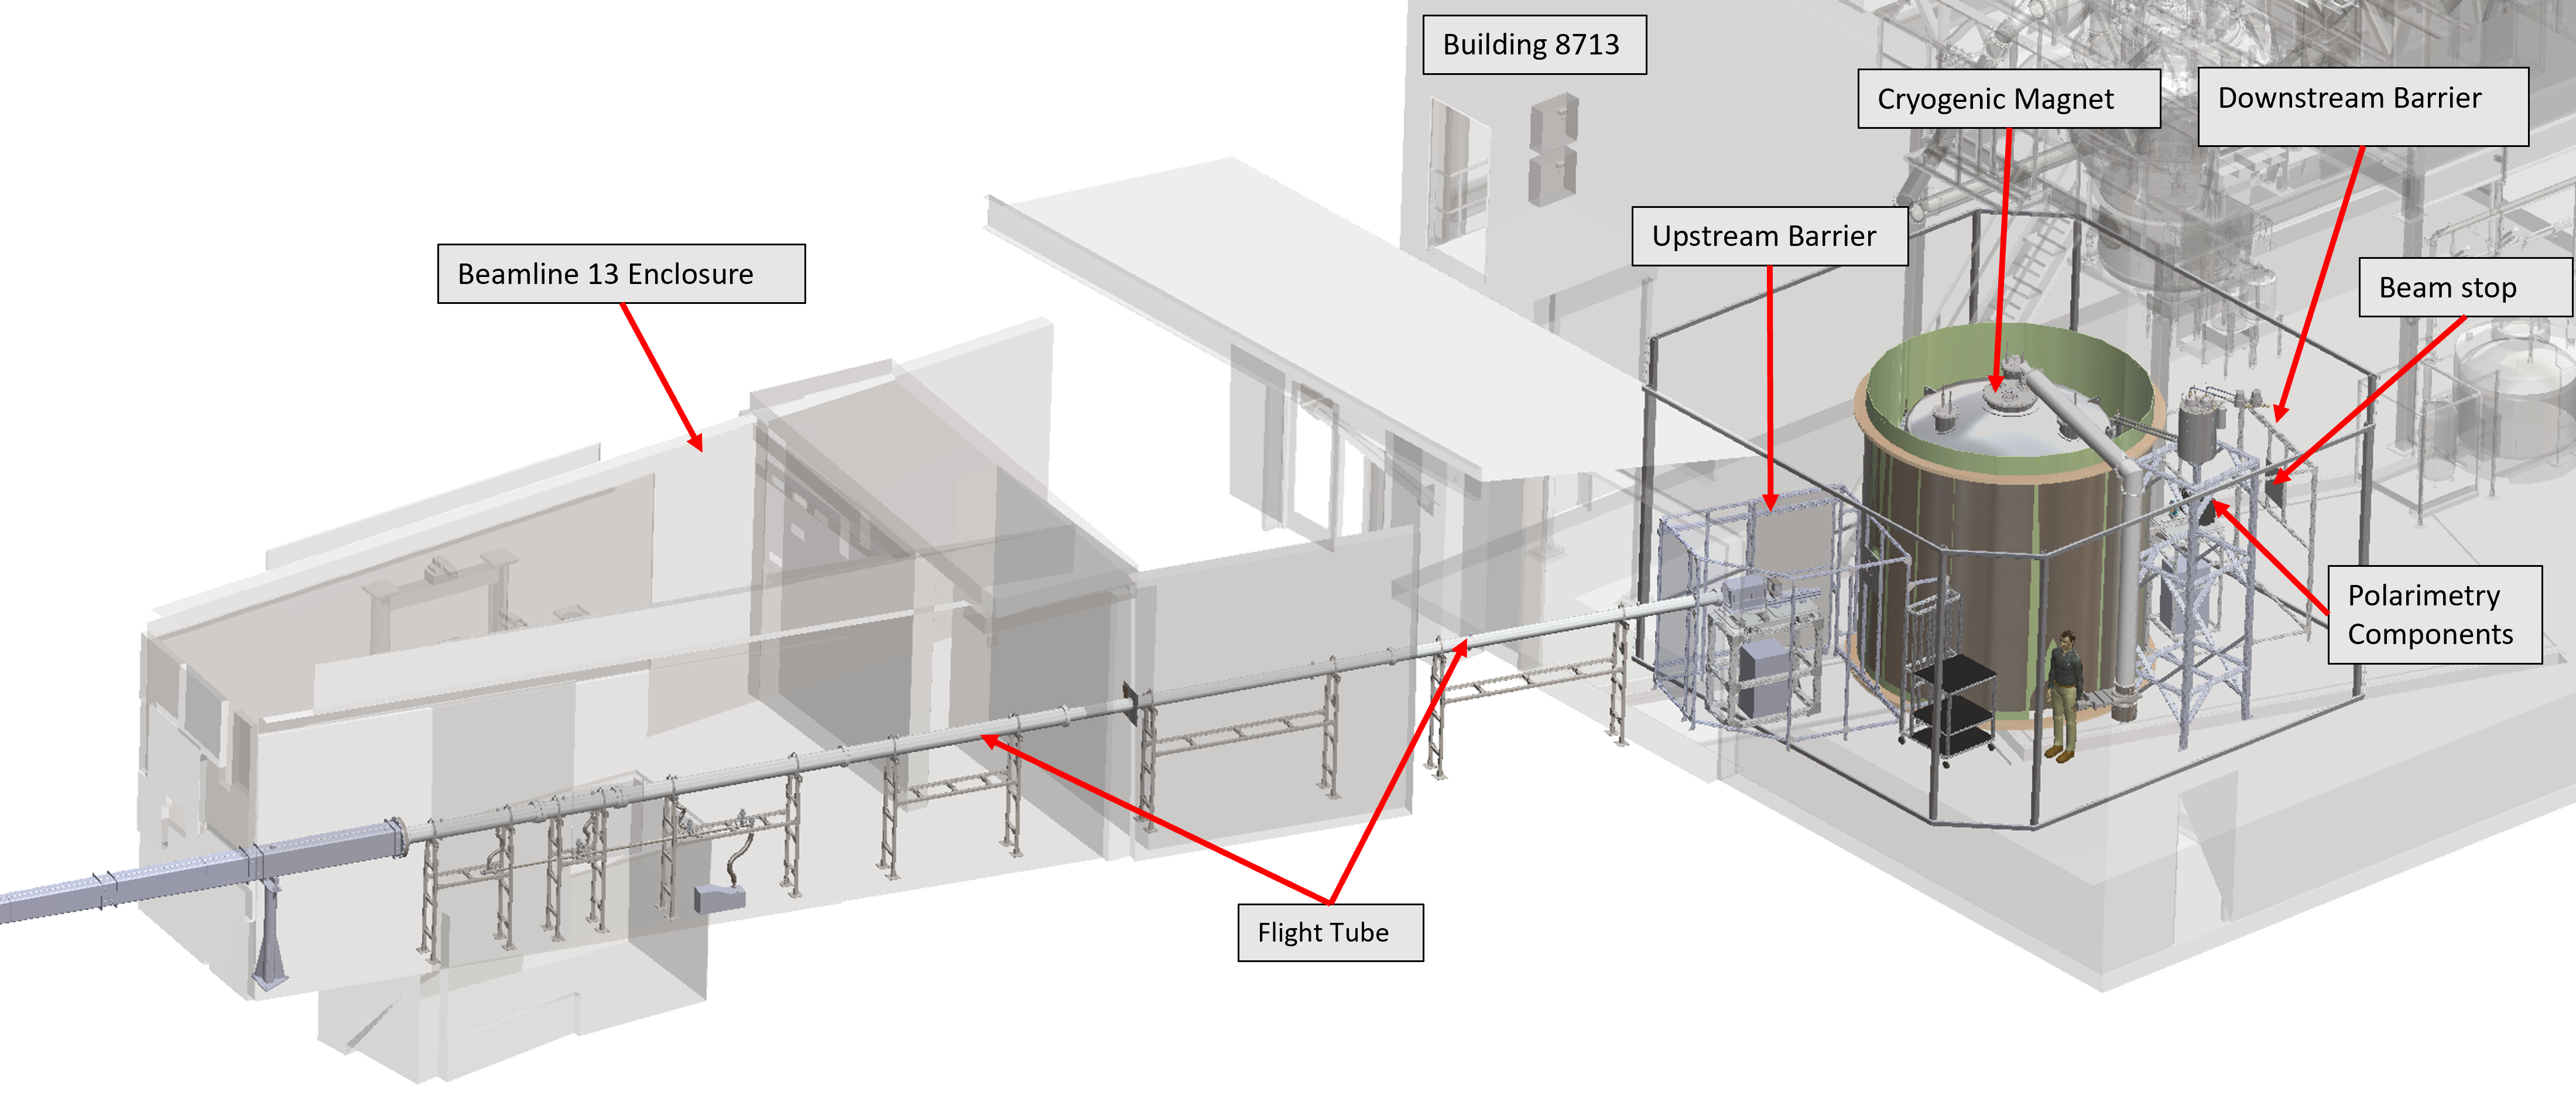
\includegraphics[width=\textwidth]{figures/chapter4-figs/Phase3pic.png}
    \caption{A CAD rendition of the polarization and transmission measurements. The figure shows the flight tube extending from the BL13 enclosure into building 8713, where the cryogenic magnet resides. The upstream and downstream barriers are where the polarimetry components will be setup for the polarization and transmission measurements.}
    \label{fig:phase3setup}
\end{figure}
\clearpage}

\subsubsection{Dose Analysis}

Because the flight tube for the polarization and transmission measurement is an extension beyond the radiological sheilding enclosure of BL13A, dosimetry analysis and measurements were needed in order to identify possible personnel safety and radiation shielding requirements. One of the important steps to commission a new beamline at the SNS is that the dosimetry analysis must indicate that the dose levels are less than the SNS unposted area limit of 0.25 mrem/hr. This analysis then undergoes a SNS facility wide safety review to obtain approval for beam operations. The majority of the radiation during the polarization and transmission measurement comes from the interaction of neutrons with materials along the flight tube geometry. As stated in \cite{Fomin2015}, the BL13A neutron beam is comprised of 8.9$\AA$ neutrons as well as $\lambda/n$ secondary wavelengths from the monochromator. Skimming of the diverging neutron beam is essential for preventing neutron capture on flight tube components. Furthermore, any unavoidable sources of neutron or gamma radiation must be shielded with materials such as lead, borated/lithiated shielding and stainless steel.

The section of the flight tube inside the beamline 13 enclosure was lined with borated shielding material on the inner face of the tube. The shielding material had a high concentration of $^{10}$B for absorption of diverging neutrons from the beam guide, preventing scattering and activation off of the Aluminium pipe and hence, reduce radiation. The flight tube outside the beamline enclosure was also made up of an aluminum pipe with five Li$_2$CO$_3$ skimmers to reduce the beam size to 5 cm in radius as well as prevent the diverging beam from creating radiation.

Monte Carlo computational programs, were utilized to sample and model both beam transport behavior and particle interaction in materials and identify radiation shielding requirements. The initial beam behavior and collimation was modeled using McStas, a Monte Carlo neutron ray-tracing program \cite{Willendrup2020}. By treating the sampled neutrons as ``ray traces" that can reflect and transmit from materials, the beam areal distribution, neutron time of flight and spectral neutron flux were modeled. This was used to optimize the collimation of the beam. All radiation and material interactions modelling was performed with MCNP6, based on the Monte-Carlo method with continuous-energy material cross sections \cite{Goorley2012}. 

A 3D model of the BL-13 enclosure with the polarization and transmission experiment as well as the neighboring Nab experiment were built in the program for accurate radiation transport and shielding calculations. The schematic layout of the proposed neutron polarization and transmission measurement as shown in \cref{fig:phase3setup} was used to develop the geometry in MCNP6 for the dose calculations. The polarizer model was developed in MCNP6 by constructing a box with the polarizer dimensions. The box was filled with boron oxide, the primary absorbing material, with a tuned density to match a 30\% neutron transmission by taking into account the loss mechanisms described above. The “polarizer” is enclosed around its length with steel to mimic the actual encasing of the box. After the polarizer, the neutron beam enters a spin flipper region, which is modeled as a double sided 5 mm thick sheet of Al. The nEDM cryogenic magnet is made of several concentric layers of cryogenic, superconductive, electrically insulating and non-magnetic materials. The neutron beam traverses the nEDM cryomagnet via thin metal beam windows made of Aluminum on the vacuum can and thermal shielding, then superconducting Pb, then low cobalt Metglas and towards the central volume. The 3 outermost layers consist of Al 6061 concentric cylinders which make up the vacuum and thermal shielding. Space between these layers is filled with $10^{-7}$ Torr air and $10^{-1}$ Torr He. The 3D model developed for Nab dosimetry studies was utilized as well to check for effects of the operations of BL13A during the Nab operation and the effects of the operation of Nab experiment towards the 13A polarization and transmission measurement. The main modifications in the Nab 3D model code were the inclusion of the flight tube and the hole in the labyrinth wall to accommodate the flight tube extension.

%This calculation also allowed for the determination of the expected neutron count rate at the end of the flight tube for the polarization and transmission measurement.

In these calculations, 2 MW average proton delivery power was assumed. BL-13A utilizes two Alkali-intercalated graphite monochromators to select 8.9~\AA\ neutrons \cite{Fomin2015}. The measured spectrum of neutrons from the monochromatic BL-13A is shown in \cref{fig:flux_wavelength}. A radially uniform source, a planar disk source with flat areal distribution, of 8.9~\AA\ neutrons was created inside MCNP6 to mimic the beam profile from BL-13A. The source is the average flux density taken from the central portion, radius of 7.62 cm, of the measured 2D beam flux as shown in \cref{fig:beam_image} of \cref{app:beamimg}. Only the neutrons from the central portion will be utilized for the measurement since there will be an initial lithium collimator at the end of the existing guide to capture the neutron flux in the corners in \cref{fig:beam_image} of \cref{app:beamimg}. The initial number of neutrons used in the source was calculated as shown in \cref{eq:MCNPflux}:
\begin{equation}
    7.24\times10^{5}~ \frac{\text{neutrons}}{\text{\AA $\cdot$ cm$^{2}$ $\cdot$ MW $\cdot$ s}} \times 0.5 ~\text{\AA} \times 2.0 ~\text{MW} \times \pi(7.62 ~\text{cm})^{2} = 1.3206\times10^{8} ~\frac{\text{neutrons}}{\text{s}}
    \label{eq:MCNPflux}
\end{equation}
By using the measured spectrum in \cite{Fomin2015}, the energies of the neutrons was set to include the 8.9~\AA\ as well as the $\lambda/2$ and $\lambda/3$ neutrons with spectral ratios of 89.5\%, 13.0\%, 0.5\% and 0.01\% for 8.9~\AA, 4.45~\AA, 2.97~\AA\ and 2.225~\AA, respectively. Beam divergence was included, where neutrons were emerging with a cone angle of $2.52\degree$ perpendicular to the source plane. For the Nab geometry, the source was taken to be the full cold neutron beam spectrum coming from BL-13B. 

%Lithium carbonate will be utilized to collimate the beam out of the flight tube. Li compounds are known to produce fast neutrons of energies up to almost 16 MeV from the n-$^6$Li decay product interaction \cite{Lone}. It is important to check whether these fast neutrons will cause a significant increase in the dose rate. This fast neutron production mechanism is missing from the MCNP6 cross section library, therefore, it has to be modeled as a new source term. To build this source term, first, the number of monochromatic neutrons absorbed in each collimators was calculated by performing an absorption cross section reaction rate tally for each of the collimators in the MCNP6 model. The number of absorbed neutrons was then multiplied by the fast neutron production rate of 1 fast neutron per $10^4$ n-Li capture products (table 2 in \cite{Lone}). These calculations are summarized in Table \ref{tab:fast}. Fig. \ref{fig:fast} shows the energy spectrum of the fast neutrons produced by thermal neutron capture in different Li compounds from \cite{Lone} \& \cite{Santoro}. This energy distribution was used in MCNP6 source term to build five isotropic point sources at the location of each of the Li collimators along the flight tube.

\Cref{fig:doseplot} shows that the calculated dose rate was less then 0.25 mrem/h, the SNS unposted area limit, outside the BL13 enclosure, eliminating the need of extra shielding. The calculations of the radiation fields for the polarization and transmission experiment on BL-13A and worst-case study simulations were also performed. The BL13 shielding enclosure was designed to keep the dose rates outside the enclosure below 0.25 mrem/h for the operation of BL-13A and BL-13B at proton beam power of 2 MW. The enclosure fulfills this requirement since MCNP6 dosimetry calculations show that gamma and neutron dose rates outside the cave walls are less than the 0.25 mrem/hr in all possible scenarios. The calculations also indicated that no area accessible to personnel has a dose rate that exceeds 0.25 mrem/hr. This led us to conclude that it is not necessary to include extra shielding other than the currently existing BL-13 enclosure and flight tube with borated shielding.

\section{Neutron Polarimetry via Polarized ${^3}$He}
\label{sec:PT}

A $^3$He NSF, which utilizes the spin dependent neutron capture on $^3$He, was used as the neutron polarization analyzer to measure the polarization of neutron beam traversing through the cryomagnet. The polarization of a neutron beam can be determined from transmission measurements through a $^3$He cell \cite{Greene1995, Musgrave2018}. $^3$He polarization and the physical properties of the $^3$He cell do not need to be known to determine the neutron polarization \cite{Greene1995}.

\begin{landscape}
\thispagestyle{mylandscape}
 \begin{figure}
    \centering
    \begin{subfigure}[b]{1.2\textwidth}
    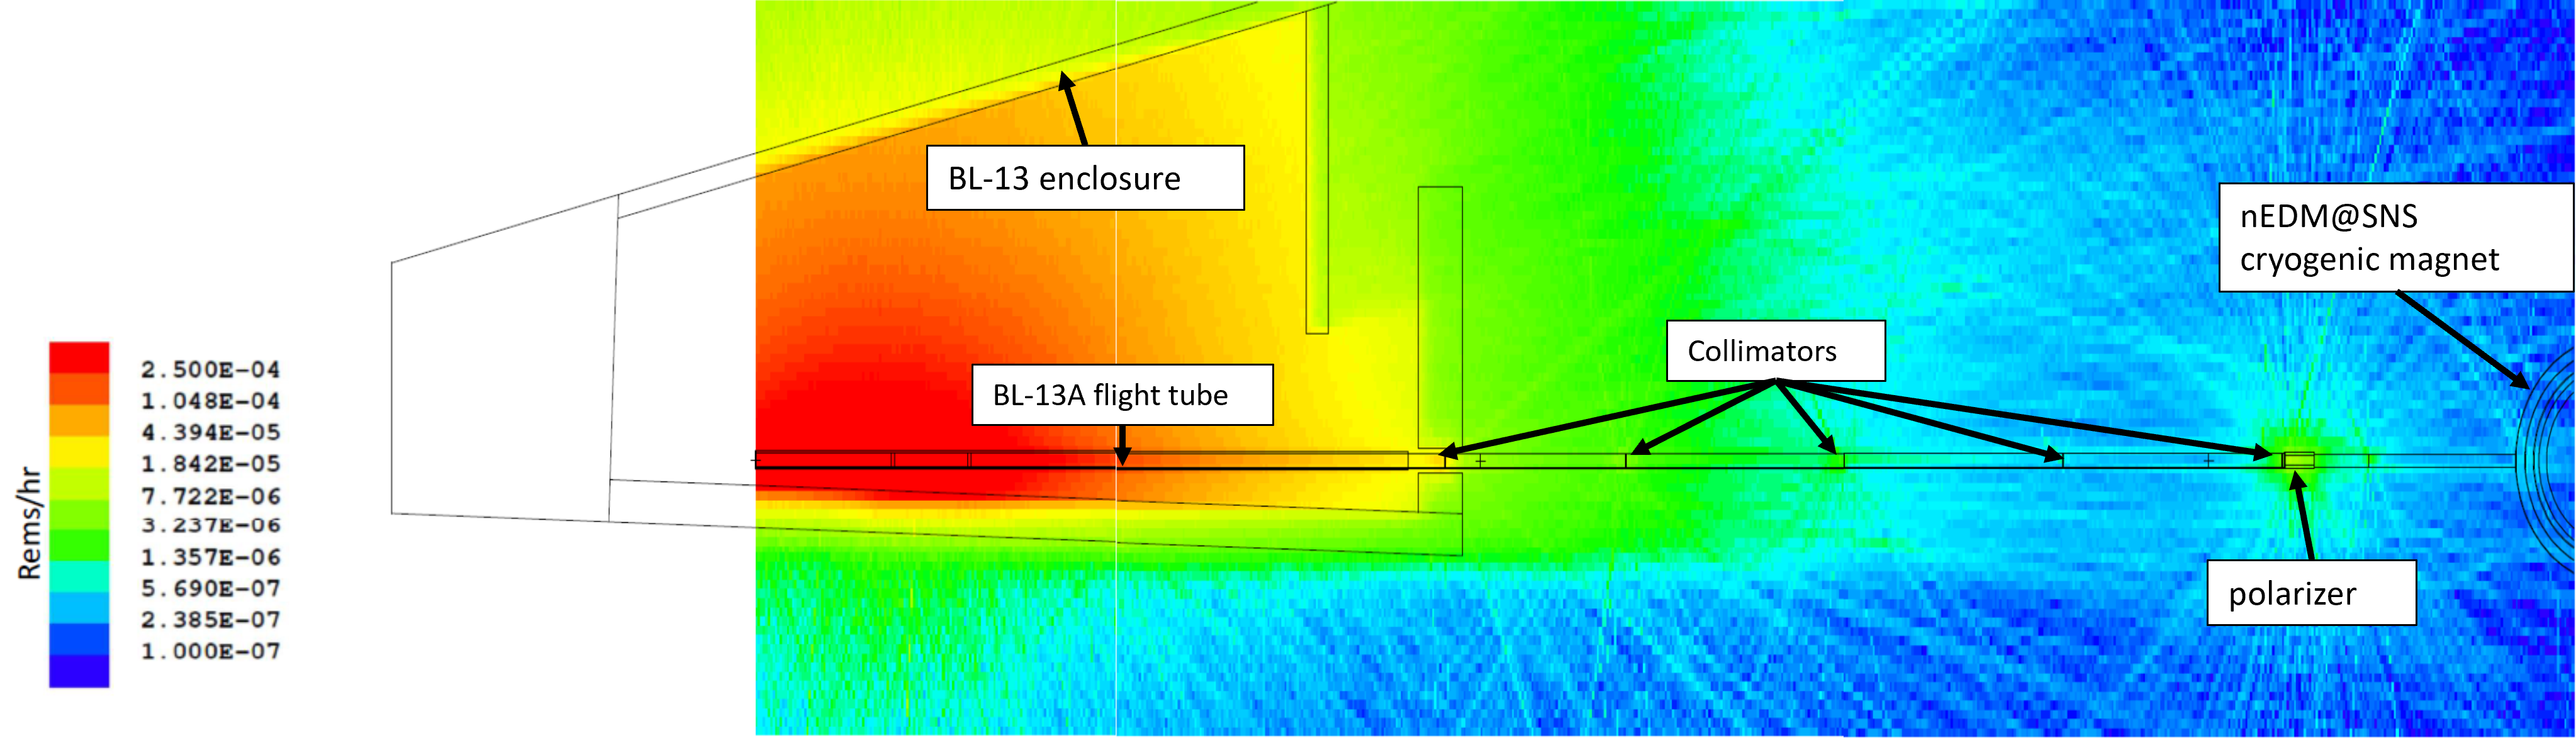
\includegraphics[width=1\linewidth]{fig3.png}
    \caption{}
    \label{fig:gammadose} 
    \end{subfigure}
    \begin{subfigure}[b]{1.2\textwidth}
    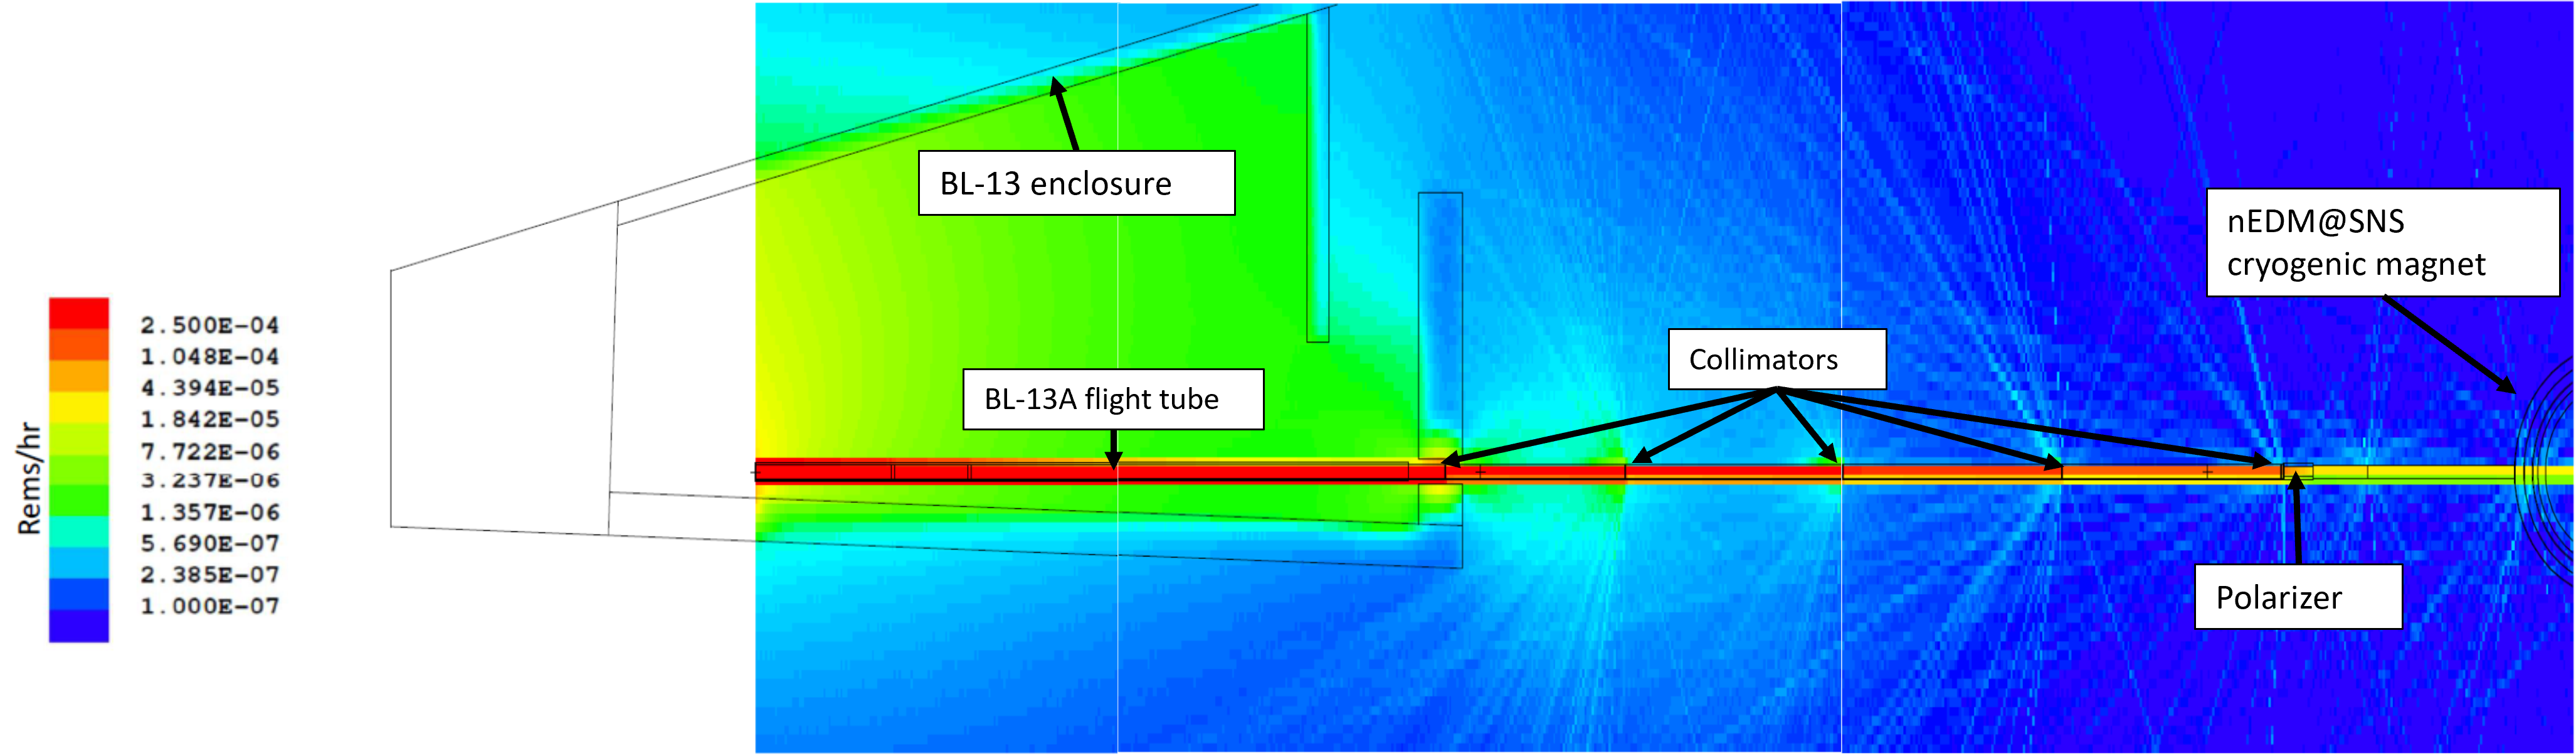
\includegraphics[width=1\linewidth]{fig4.png}
    \caption{}
    \label{fig:neutrondose}
    \end{subfigure}
\caption{Dose rate heat maps of the 3D model of proposed neutron polarization transmission measurement at BL-13A simulated in MCNP6. The figure shows a top down view of the the extension of BL-13A via flight tubes towards the SNS building 8713, the Neutron polarizer and the nEDM cryogenic magnet. The gamma ray dose rate is shown in (a) and the neutron dose rate is shown in (b). The units of dose rate are in [rem/hr] with the color red set to be above the SNS unposted area limit of $2.5\times10^{-4}$ rem/hr.}
\label{fig:doseplot}
\end{figure}   
\end{landscape}

As previously described in \cref{ch:polHe}, the transmission of neutrons through a 3He cell is determined from:
\begin{equation}\label{eq:tzero}
    T_0=T_e e^{-\zeta}
\end{equation} 
where $\zeta$ is the opacity defined in \cref{eq:opacity}. The transmission of spin up ($\uparrow$) and spin down ($\downarrow$) neutrons through a polarized $^3$He analyzer with polarization $P_{He}$ (by making initial neutron polarization implicit) becomes:
\begin{equation}
    T_\uparrow = N_0\frac{\left(1+P_n\right)}{2}e^{-\zeta (1-P_{He})}
\end{equation}
\begin{equation}
    T_\downarrow = N_0\frac{\left(1-P_n\right)}{2}e^{-\zeta (1+P_{He})}
\end{equation}
Hence the total transmission of a polarized neutron beam through polarized $^3$He analyzer becomes:
\begin{equation}\label{eq:t}
    T = T_\uparrow + T_\downarrow = N_0e^{-\zeta}\cosh{\left(\zeta P_{He}\right)}\left[1+P_n\tanh{\left(\zeta P_{He}\right)}\right]
\end{equation}
To obtain the other spin state, a neutron spin flipper is used to rotate the spins by $\pi$ radians with efficiency $\epsilon_{sf}\leq1$. The magnitude of the neutron polarization becomes $(1-2\epsilon_{sf})P_n$: 
\begin{equation}\label{eq:tsf}
    T_{sf} = N_0e^{-\zeta}\cosh{\left(\zeta P_{He}\right)}\left[1+\left(1-2\epsilon_{sf}\right)P_n\tanh{\left(\zeta P_{He}\right)}\right]
\end{equation}

The neutron polarization, $P_n$ can be determined from three transmission measurements, neutron transmission through unpolarized $^3$He ($T_0$ in \cref{eq:tzero} ) and transmission through polarized $^3$He for both neutron spin states ($T$ in \cref{eq:t} and $T_{sf}$ in \cref{eq:tsf}). The ratio of the neutron transmission through polarized and unpolarized $^3$He eliminates various non-ideal systematic errors arising from the neutron detector. If we define the ratio of $T$ with $T_0$ as $R$, the ratio of $T_{sf}$ with $T_0$ as $R_{sf}$:
\begin{equation}\label{eq:R}
    R = \frac{T}{T_0} = \cosh{\left(\zeta P_{He}\right)}\left[1+P_n\tanh{\left(\zeta P_{He}\right)}\right]
\end{equation}
\begin{equation}\label{eq:Rsf}
    R_{sf} = \frac{T_{sf}}{T_0} = \cosh{\left(\zeta P_{He}\right)}\left[1+\left(1-2\epsilon_{sf}\right)P_n\tanh{\left(\zeta P_{He}\right)}\right]
\end{equation}
By using the trigonometric identity, $1 - \tanh^2{x} = \sech^2{x}$, and substituting in \cref{eq:R} and \cref{eq:Rsf} to solve for $\cosh{\zeta}$:
\begin{equation}
    \cosh{\zeta} = \frac{1}{2\epsilon_{sf}}\left[R_{sf}-(1-2\epsilon_{sf})R\right]
\end{equation}
This result allows \cref{eq:R} and \cref{eq:Rsf} to become:
\begin{equation}\label{eq:R_nocosh}
    R = \frac{1}{2\epsilon_{sf}}\left[R_{sf}-(1-2\epsilon_{sf})R\right] - P_n\sqrt{\left[\frac{1}{2\epsilon_{sf}}\left[R_{sf}-\left(1-2\epsilon_{sf}\right)R\right]\right]^2 -1}
\end{equation}
\begin{equation}\label{eq:Rsf_nocosh}
    R_{sf} = \frac{1}{2\epsilon_{sf}}\left[R_{sf}-\left(1-2\epsilon_{sf}\right)R\right] - \left(1-2\epsilon_{sf}\right)P_n\sqrt{\left[\frac{1}{2\epsilon_{sf}}\left[R_{sf}-\left(1-2\epsilon_{sf}\right)R\right]\right]^2 -1}
\end{equation}
From \cref{eq:R_nocosh} and \cref{eq:Rsf_nocosh}, the polarization of neutrons can be determined simply as function of neutron transmission ratios and spin flipper efficiency $\epsilon_{sf}$:
\begin{equation} \label{eq:polarization}
P_n=\frac{R-R_{sf}}{\sqrt{\left[\left(2\epsilon_{sf}-1\right)R+R_{sf}\right]^{2}-4\epsilon_{sf}^2}}
\end{equation}

\subsection{Efficiency of spin flipper}

The spin-flip efficiency, $\epsilon_{sf}$ , can be determined from four transmission measurements: two with the initial neutron spin state, $T$ and $T^{AFP}$, and another two with the neutrons spin flipped, $T_{sf}$ and $T^{AFP}_{sr}$ for both $^3$He polarization states. AFP corresponds to transmission measurements where the $^3$He polarization was reversed by adiabatic fast passage (AFP). Four transmission measurements give the ratios $R$ and $R_{sf}$:
\begin{equation}
    \frac{T^{AFP}-T}{T^{AFP}+T} = P_n\tanh{\left(\zeta P_{He}\right)} = R
\end{equation}
\begin{equation}
    \frac{T^{AFP}_{sr}-T_{sf}}{T^{AFP}_{sr}+T_{sf}} = \left(1-2\epsilon_{sf}\right)P_n\tanh{\left(\zeta P_{He}\right)} = R_{sf}
\end{equation}
The spin flipper efficiency can be calculated from these ratios as:
\begin{equation}
\begin{split}
    \epsilon_{sf} & = \frac{1}{2} \left( 1 - \frac{R_{sf}}{R}  \right) \\
    & =\frac{1}{2} \left(1-\frac{\frac{T^{AFP}_{sr}-T_{sf}}{T^{AFP}_{sr}+T_{sf}}}{\frac{T^{AFP}-T}{T^{AFP}+T}}\right) 
\end{split}
\end{equation}

An important note needs to be made here. To polarize the neutron, a neutron polarizing device is employed. Since the polarization of the beam is defined based on the guiding magnetic field, guiding magnetic field components have to be used to maintain the polarization and provide spin transport from the polarizing device to the analyzing device. It is also important to characterize the spin flipped state, so a spin flipper is also utilized. Therefore, the neutron beam polarization is actually the product of the spin transport efficiency, $\epsilon_{ST}$, the spin flipper efficiency, $\epsilon_{SF}$, the spin polarizing power of the neutron polarizer, $P_{n}$, and the spin analyzing power, $P^{He}_{n}$, of the spin analyzer as:
\begin{equation}
    \epsilon_{ST} \cdot \epsilon_{SF} \cdot P_{n} \cdot P^{He}_{n} = \frac{R_{\uparrow}-R_{\downarrow}}{R_{\uparrow}+R_{\downarrow}}
\end{equation}
Since the beam polarization is set by the neutron polarizer and defined by the spin transport, $P_{n}$ and $\epsilon_{ST}$ cannot separated. Therefore, the beam polarization is defined as:
\begin{equation}
    \epsilon_{ST} \cdot P_{n} \rightarrow P_{n} = \frac {1}{ \epsilon_{SF} \cdot P^{He}_{n} } \left( \frac{R_{\uparrow} - R_{\downarrow}}{R_{\uparrow}+R_{\downarrow}}  \right) =  \frac{R_{\uparrow} - R_{\downarrow}}{ \sqrt{ \left(\left(2\epsilon_{sf}-1\right)R_\uparrow + R_\downarrow \right)^2 - 4\epsilon_{SF}^2 }  } 
\end{equation}
where $ \epsilon_{SF} = \frac{1}{2} \left(  1 - \frac{R_\downarrow}{R_\uparrow}     \right) $, is the efficiency of the spin flipper used to flip $R_\uparrow$ to $R_\downarrow$.

\section{Experimental Setup and Measurement Scheme}

This section will cover the experimental setup for the different configurations used to measure the transmission and polarization loss from the cryomagnet. The first configuration was to measure the neutron transmission loss from the cryomagnet. This setup is illustrated in \cref{fig:trans_setup}. The objective here is to measure the neutron beam intensity before the cryomagnet and then after the cryomagnet. The ratio of the transmissions will determine the fraction of neutron beam lost due to the presence of the cryomagnet. First, the neutron beam was defined based on the two $^6$Li apertures with 2 cm by 2 cm opening. The placement and opening of these apertures lock in the beam cross sectional area going into the cryomagnet. To measure the neutron intensity before the cryomagnet, the neutron detector was placed upstream of the cryomagnet, as shown in \cref{fig:upstream_trans}. To measure the neutron intensity after the cryomagnet, the same neutron detector was placed downstream of the cryomagnet as shown in \cref{fig:downstream_trans}. It is crucial for the apertures to ensure that the neutrons detected in the upstream configuration are the same neutrons that traverse the cryomagnet and are detected at the downstream configuration.

\afterpage{
\begin{figure}
\centering
  \begin{subfigure}[]{\textwidth}
    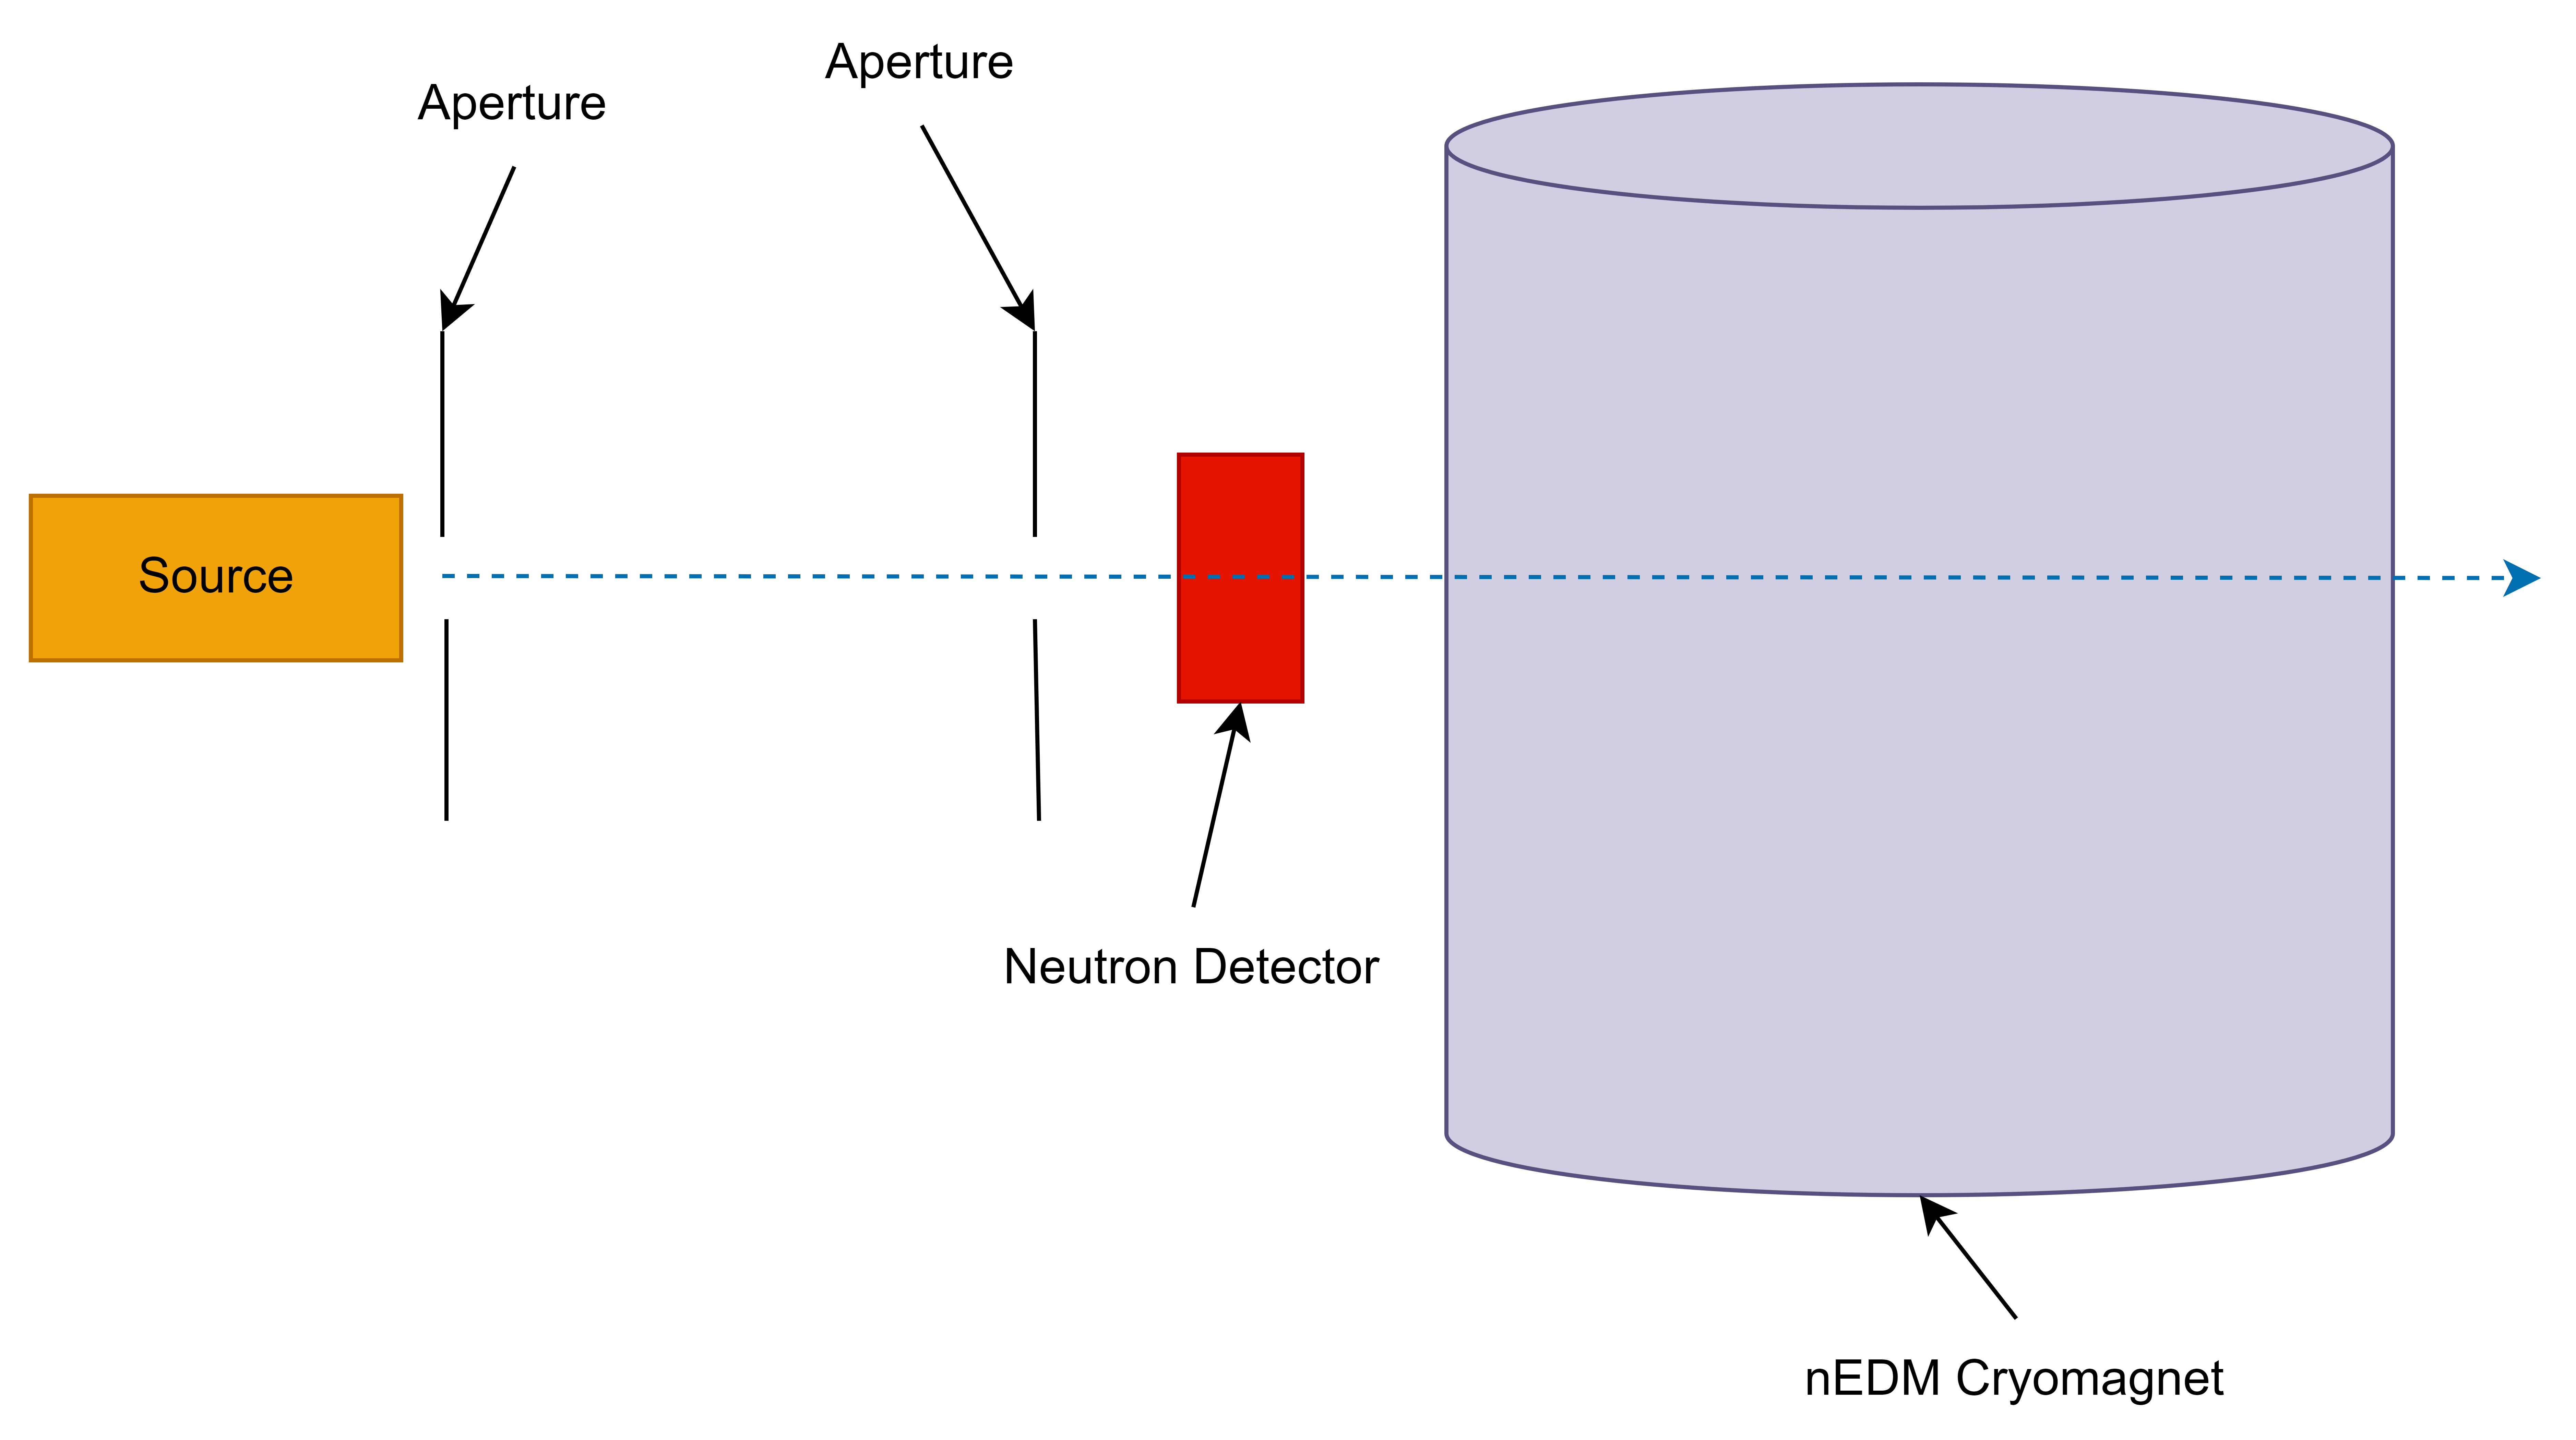
\includegraphics[width=\textwidth]{figures/chapter4-figs/upstream_trans.png}
    \caption{}
    \label{fig:upstream_trans}
  \end{subfigure}
  \hfill
  \begin{subfigure}[]{\textwidth}
    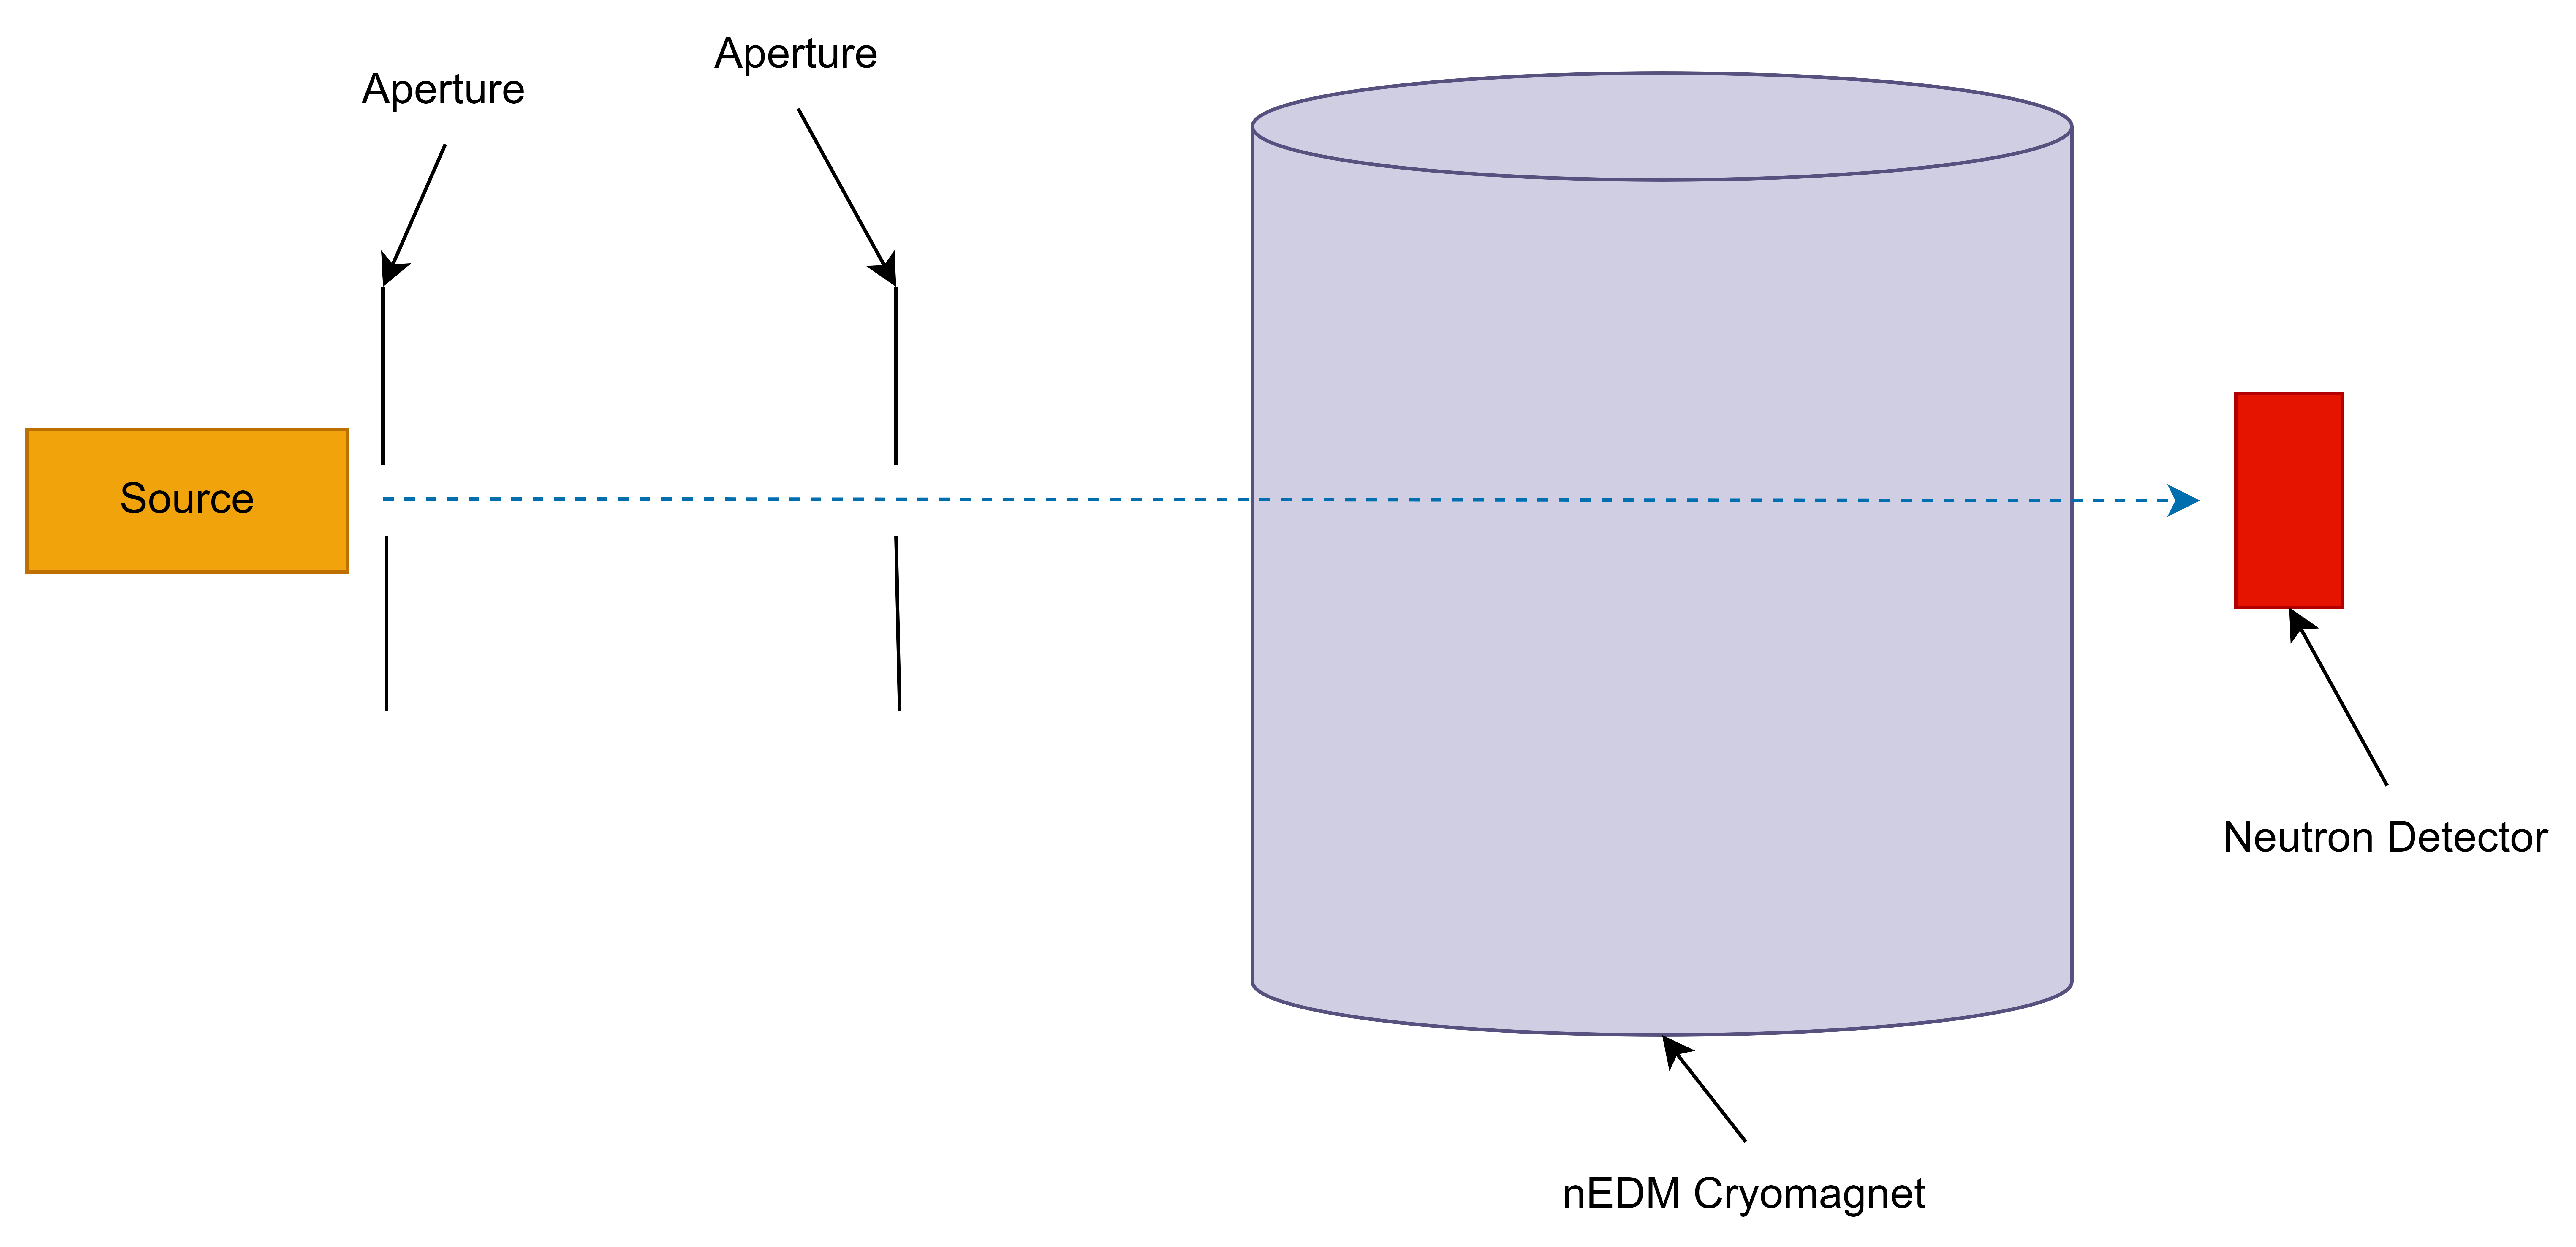
\includegraphics[width=\textwidth]{figures/chapter4-figs/downstream_trans.png}
    \caption{}
    \label{fig:downstream_trans}
  \end{subfigure}
  \caption{A schematic setup to measure the transmission loss of neutron beam through the nEDM cryomagnet by measuring the initial beam in (a) and after beam in (b). Here the component "Source" refers to the neutron flight tube. The blue dotted arrow represents the neutron beam.}
  \label{fig:trans_setup}
\end{figure}
\clearpage}

\afterpage{
\begin{figure}
\centering
  \begin{subfigure}[]{\textwidth}
    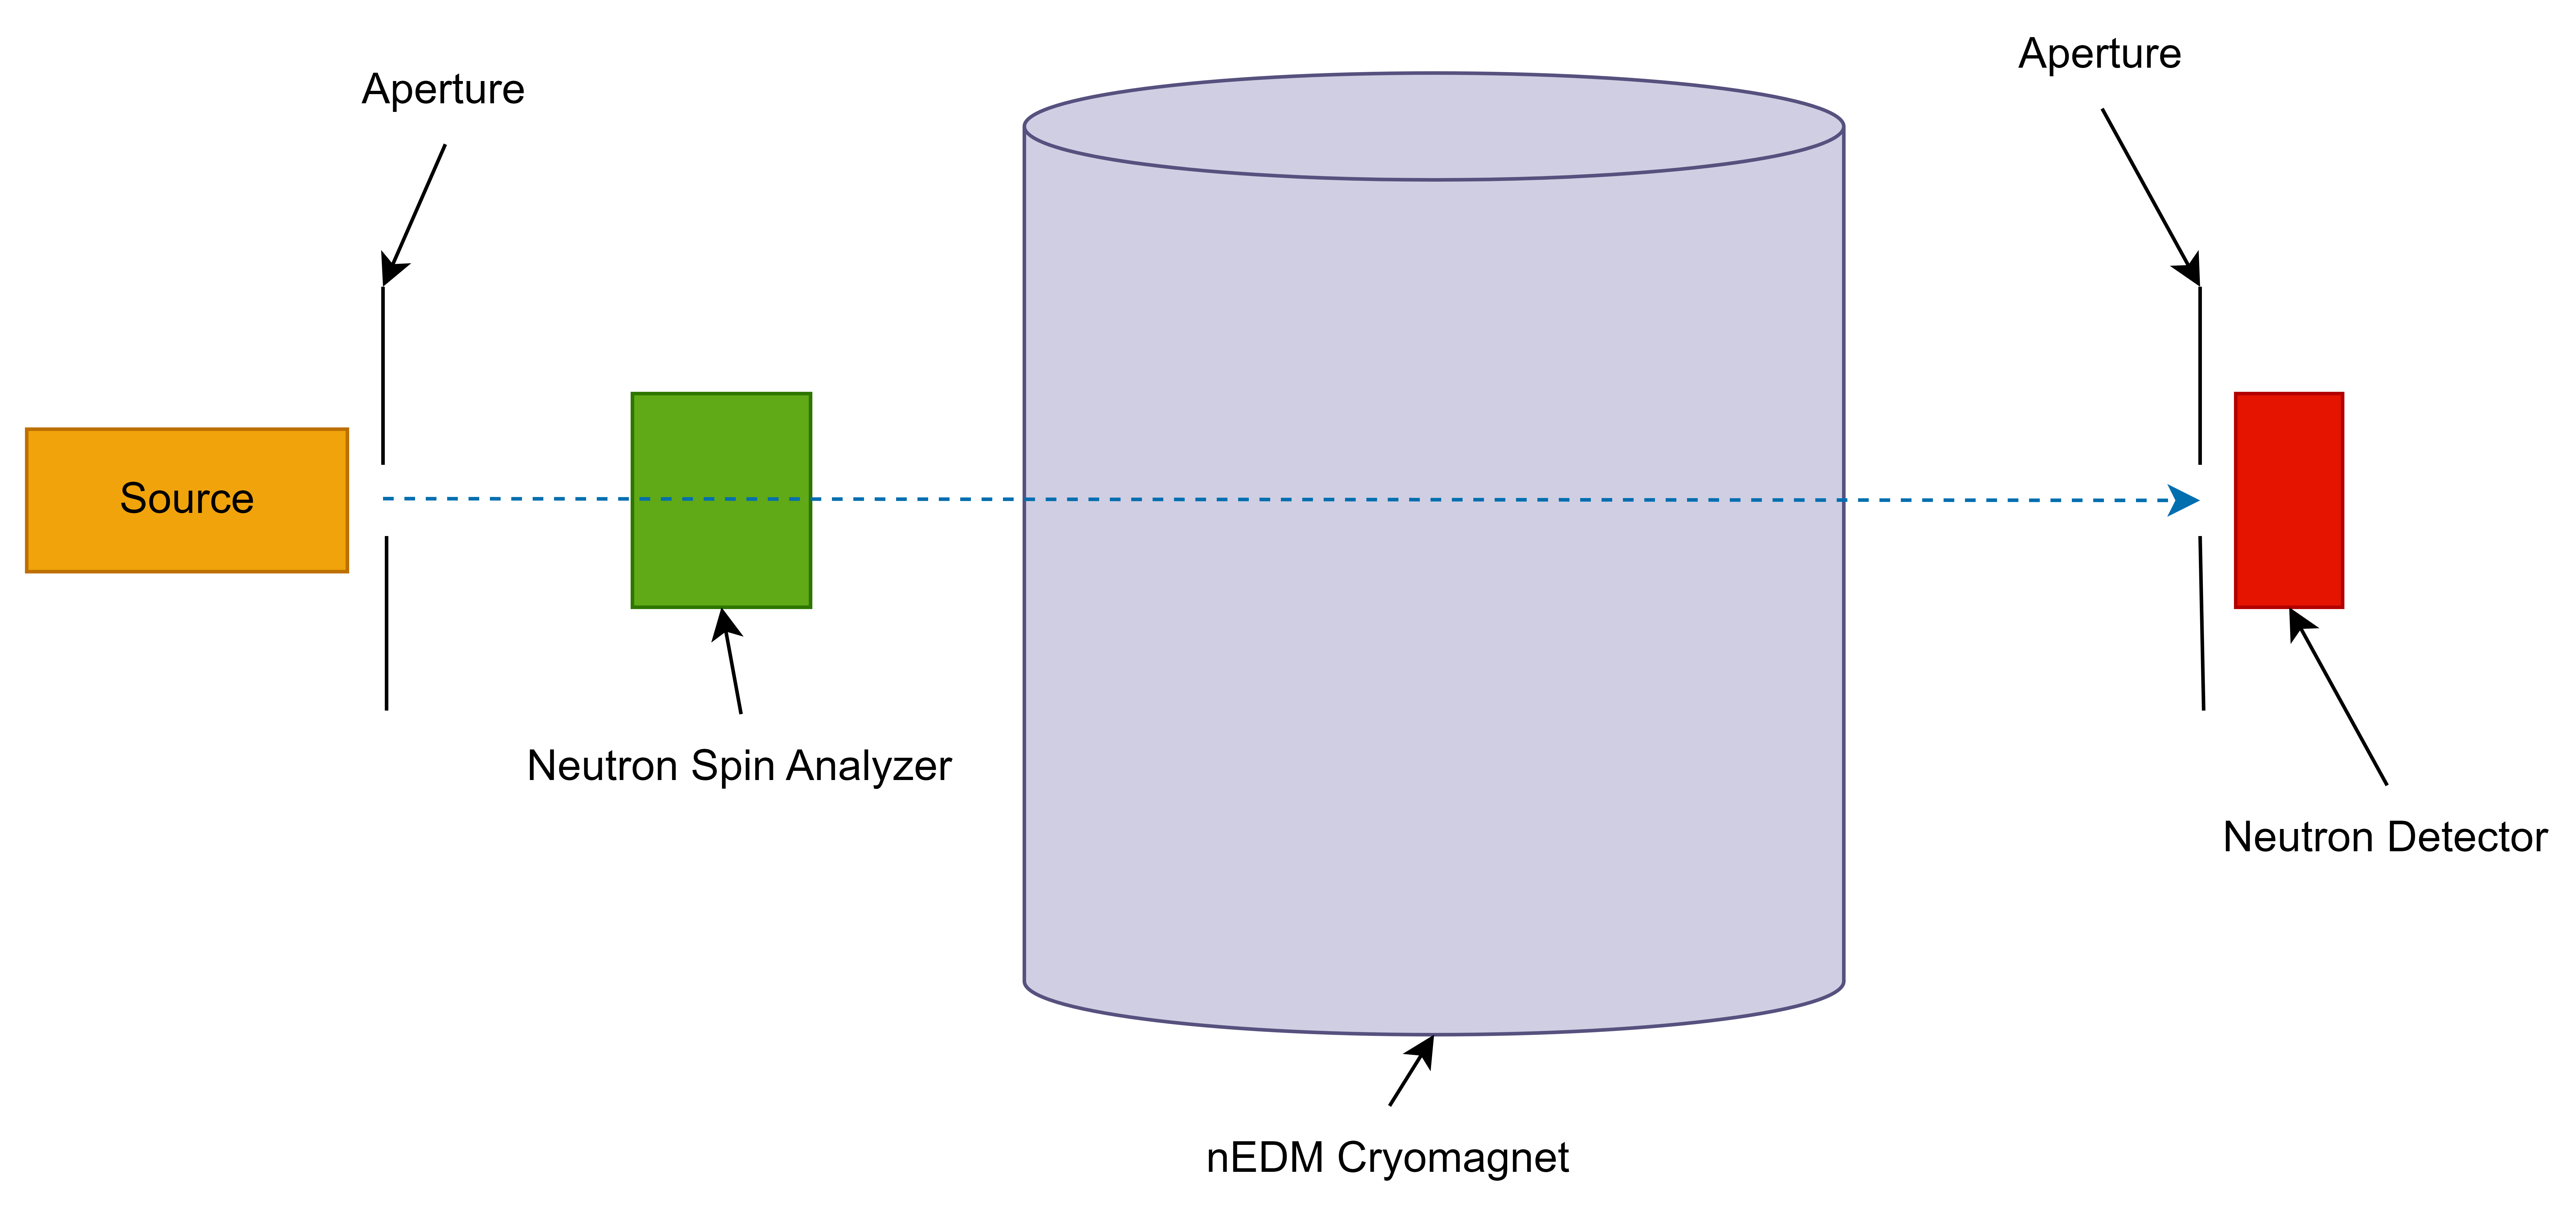
\includegraphics[width=\textwidth]{figures/chapter4-figs/upstream_polarimetry.png}
    \caption{}
    \label{fig:upstream_pol}
  \end{subfigure}
  \hfill
  \begin{subfigure}[]{\textwidth}
    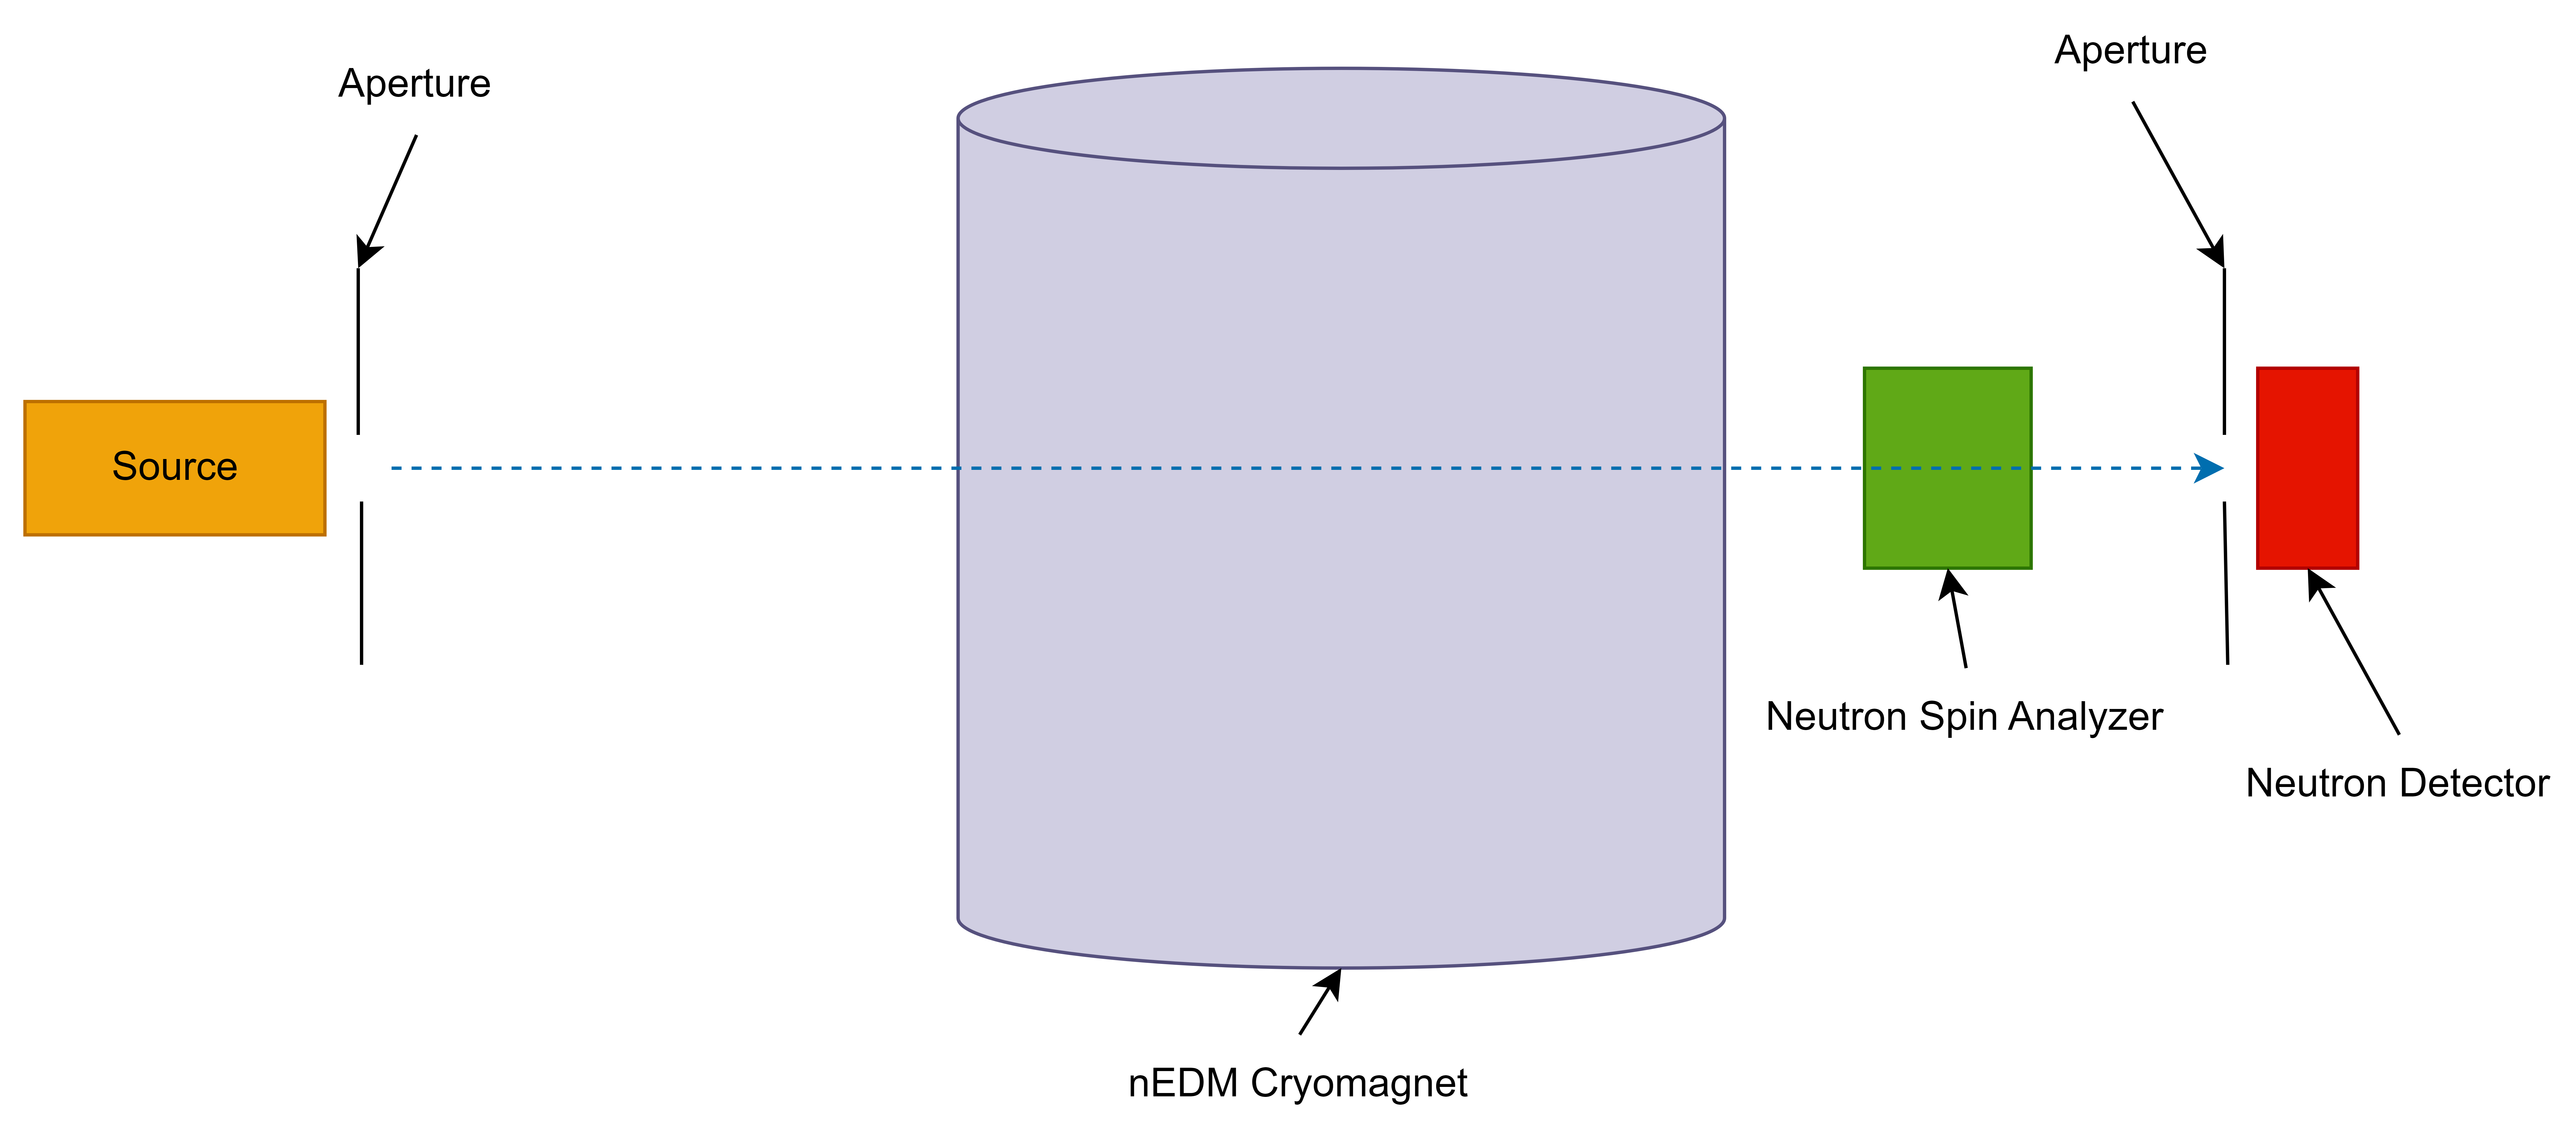
\includegraphics[width=\textwidth]{figures/chapter4-figs/downstream_polarimetry.png}
    \caption{}
    \label{fig:downstream_pol}
  \end{subfigure}
  \caption{A schematic setup for the (a) upstream polarimetry measurement and (b) downstream polarimetry measurement. Here the component "Source" refers to the neutron polarizer and neutron spin flipper. The blue dotted arrow represents the polarized neutron beam.}
  \label{fig:polarimetry_setup}
\end{figure}
\clearpage}

The second setup was to measure the neutron polarization loss from the cryomagnet via transmission of neutrons through the $^3$He analyzer for neutron polarimetry based on \cref{eq:polarization}. \Cref{fig:polarimetry_setup} illustrates the setup used to measure the polarization of the neutron beam before and after the cryomagnet. The difference between the measured polarization upstream of the cryomagnet and downstream of the cryomagnet will be used to determine the contribution of the cryomagnet windows and its magnetic fields to neutron polarization loss. The initial beam emerging from the flight tube is unpolarized, therefore, a neutron polarizer is placed to polarize the neutron beam. Then a neutron spin flipper is placed after the polarizer. The flipper is placed to account for its contribution towards beam intensity loss as the beam traverses through it but it is only activated when the measurement configuration call for it. For the entire neutron polarimetry run, the neutron detector was placed downstream of the cryomagnet. The neutron beam was defined by two $^6$Li apertures with 2 cm by 2 cm opening, first one placed after the spin flipper and the second one placed right before the neutron detector. The placement and opening of these apertures ensures that polarized neutrons are going the $^3$He neutron spin analyzer. A caveat of this measurement scheme is the assumption that the neutrons were polarized uniformly along the entire phase space of the defined neutron beam. To measure the neutron polarization before the cryomagnet, the neutron spin analyzer was placed upstream of the cryomagnet, as shown in \cref{fig:upstream_pol}. To measure the  neutron polarization after the cryomagnet, the neutron spin analyzer was placed downstream of the cryomagnet as shown in \cref{fig:downstream_pol}. To measure the neutron beam polarization upstream and downstream, neutron beam polarization and neutron spin analyzer configurations as shown in \cref{fig:pol_scheme} were used. These configuration are as follows:
\begin{enumerate}
    \item First, as shown \cref{fig:directbeam}, the transmission of the polarized neutron beam without the $^3$He neutron spin analyzer was measured.
    \item Second, as shown \cref{fig:unpolcell}, the transmission of the polarized neutron beam with an unpolarized $^3$He neutron spin analyzer was measured.
    \item Third, as shown \cref{fig:polbeam}, the transmission of the polarized neutron beam with a polarized $^3$He neutron spin analyzer (the beam polarization is parallel relative to the polarized $^3$He) was measured. This is called the high transmission spin state of the spin analyzer.
    \item Fourth, as shown \cref{fig:sfbeam_polcell}, the transmission of the spin flipped neutron beam with a polarized $^3$He neutron spin analyzer (the beam polarization is anti-parallel relative to the polarized $^3$He) was measured. The neutron beam spin was flipped using a neutron spin flipper. This measurement is called the low transmission spin state of the spin analyzer.
    \item Fifth, as shown \cref{fig:polbeam_afpcell}, the transmission of the polarized neutron beam with an anti-polarized $^3$He neutron spin analyzer was measured. The polarized $^3$He was inverted using the AFP technique described in \cref{ch:polHe}
    \item Sixth, as shown \cref{fig:sfbeam_afpcell}, the transmission of the spin flipped neutron beam with an anti-polarized $^3$He neutron spin analyzer was measured.
\end{enumerate}
The transmission of polarized neutrons through the neutron spin analyzer based on these above configurations will determine the relevant transmission ratios needed to extract the neutron beam polarization using \cref{eq:polarization}. The neutron polarizing instruments and the neutron detector are described in detail the following sections.



\afterpage{
\begin{figure}
    \centering
    \begin{subfigure}[b]{0.6\linewidth}
        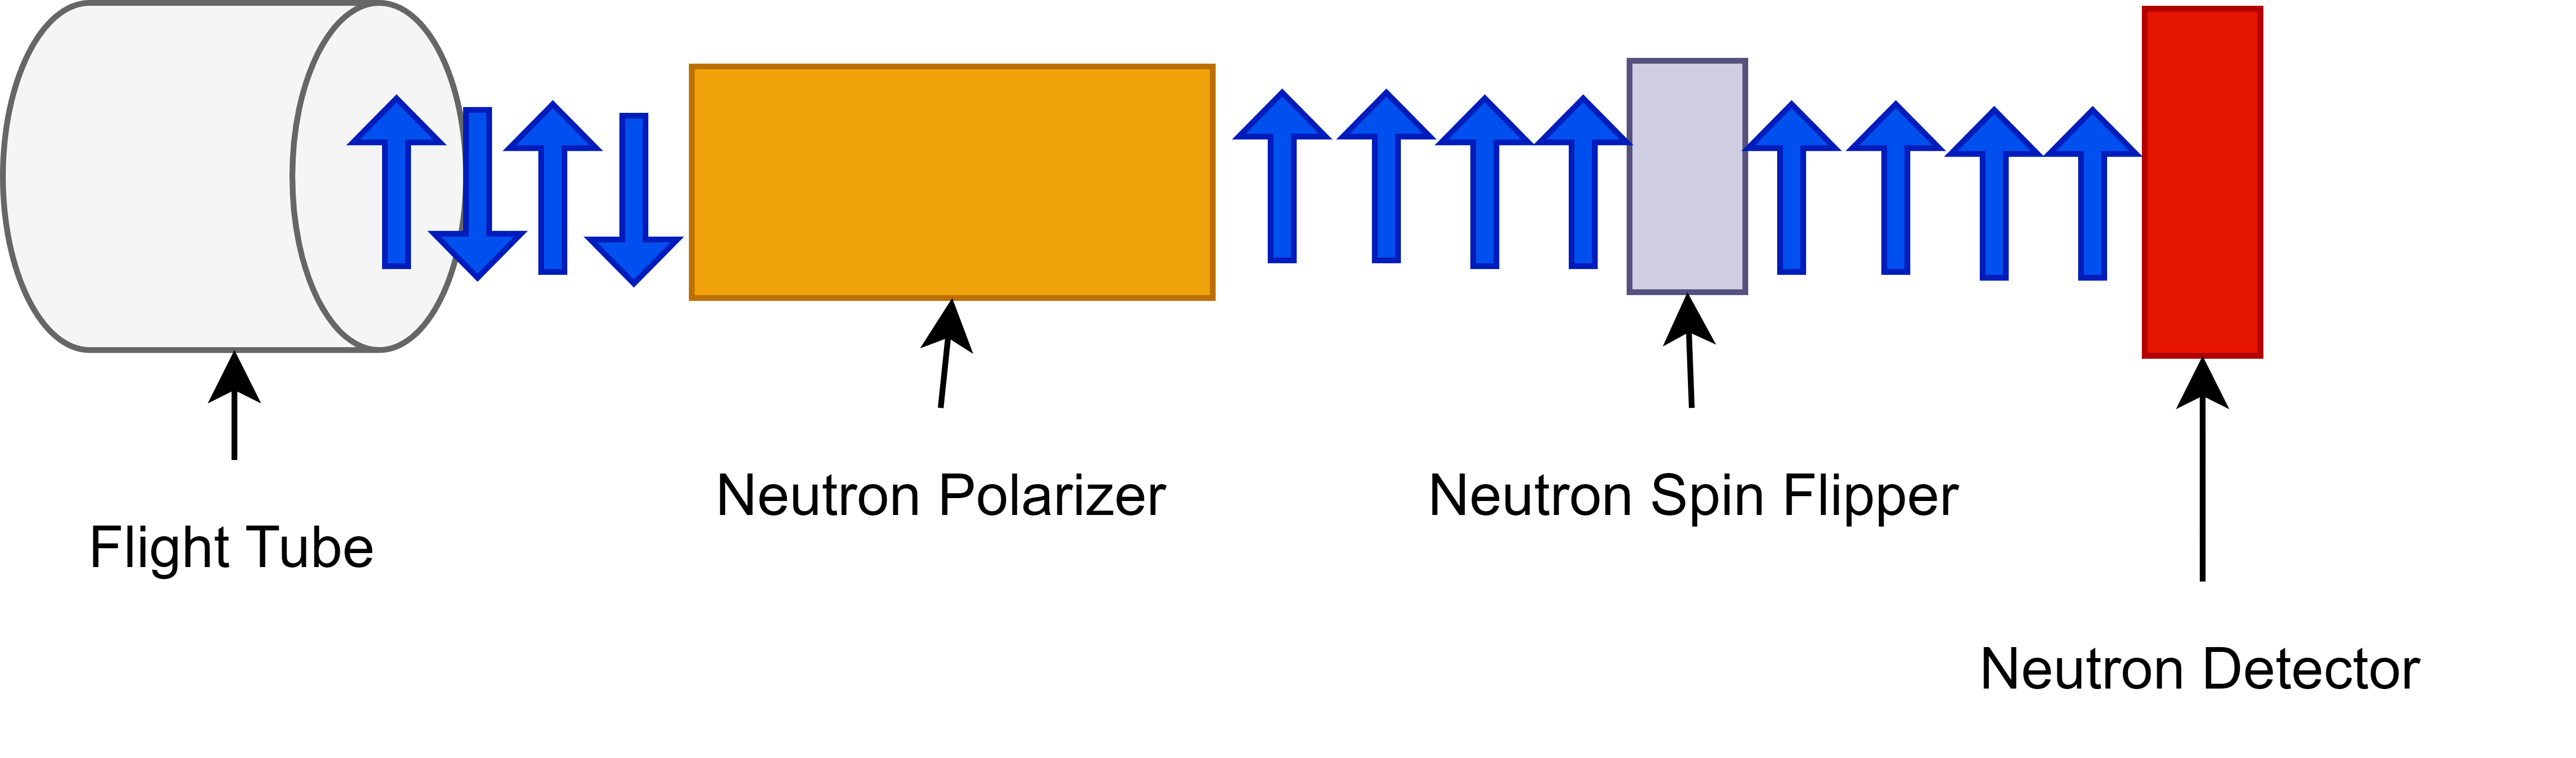
\includegraphics[width=\linewidth, height=2.5cm]{noanalyzer.png}
    \caption{$N_0$}
    \label{fig:directbeam}
    \end{subfigure}
    \hfil
    \begin{subfigure}[b]{0.75\linewidth}
        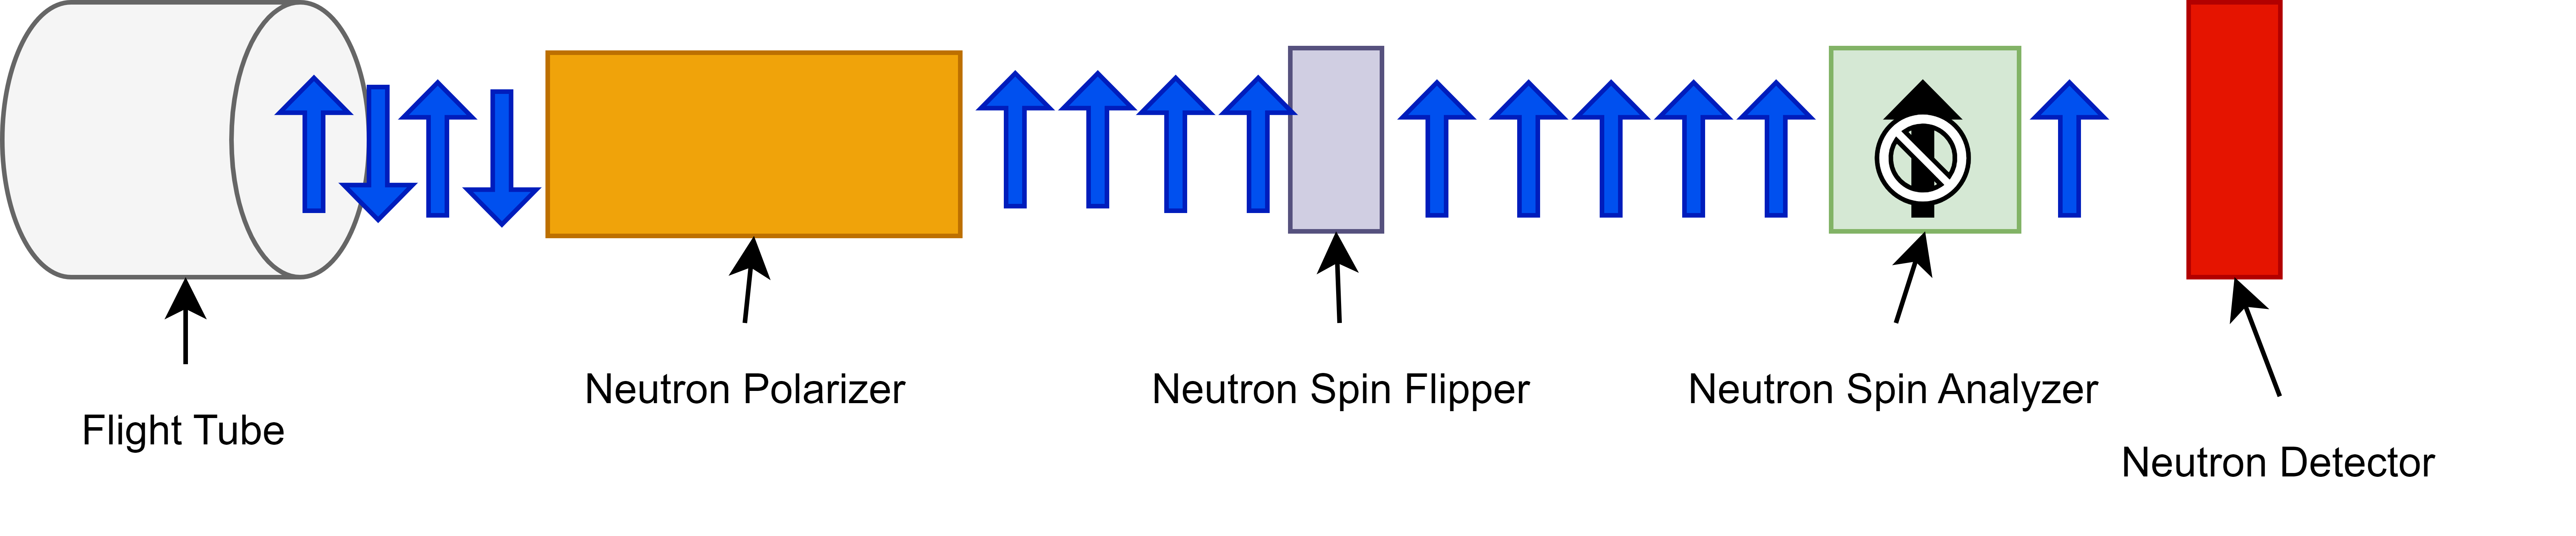
\includegraphics[width=\linewidth, height=2.5cm]{figures/chapter4-figs/unpolarizedcell.png}
    \caption{$T_0$}
    \label{fig:unpolcell}
    \end{subfigure}

    \begin{subfigure}[b]{0.75\linewidth}
        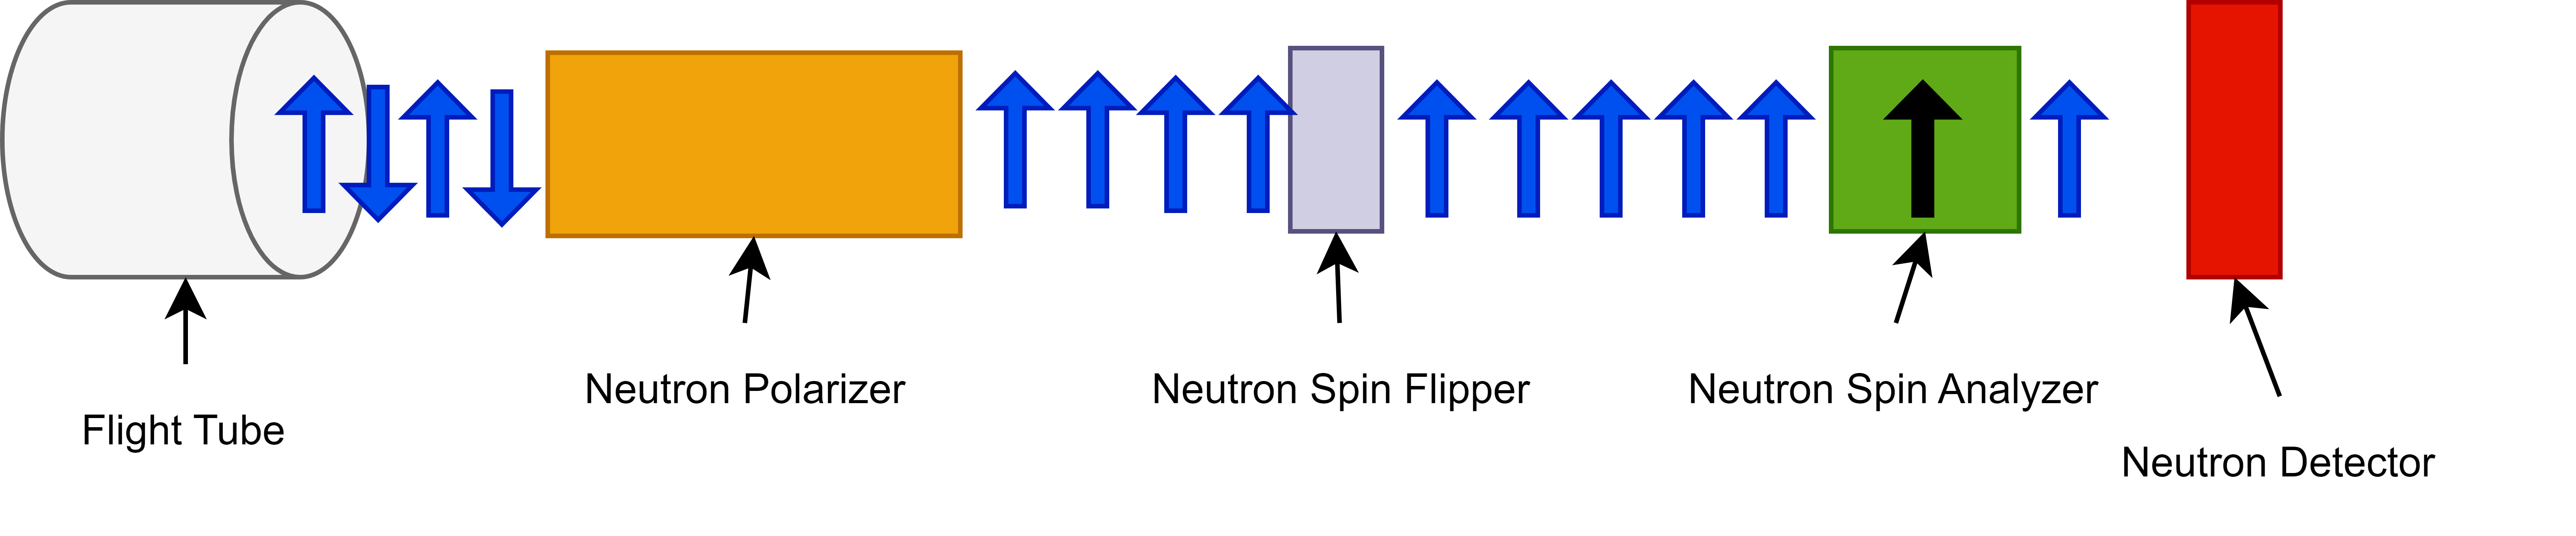
\includegraphics[width=\linewidth, height=2.5cm]{figures/chapter4-figs/polbeam.png}
    \caption{$T$}
    \label{fig:polbeam}
    \end{subfigure}
    \hfil
    \begin{subfigure}[b]{0.75\linewidth}
        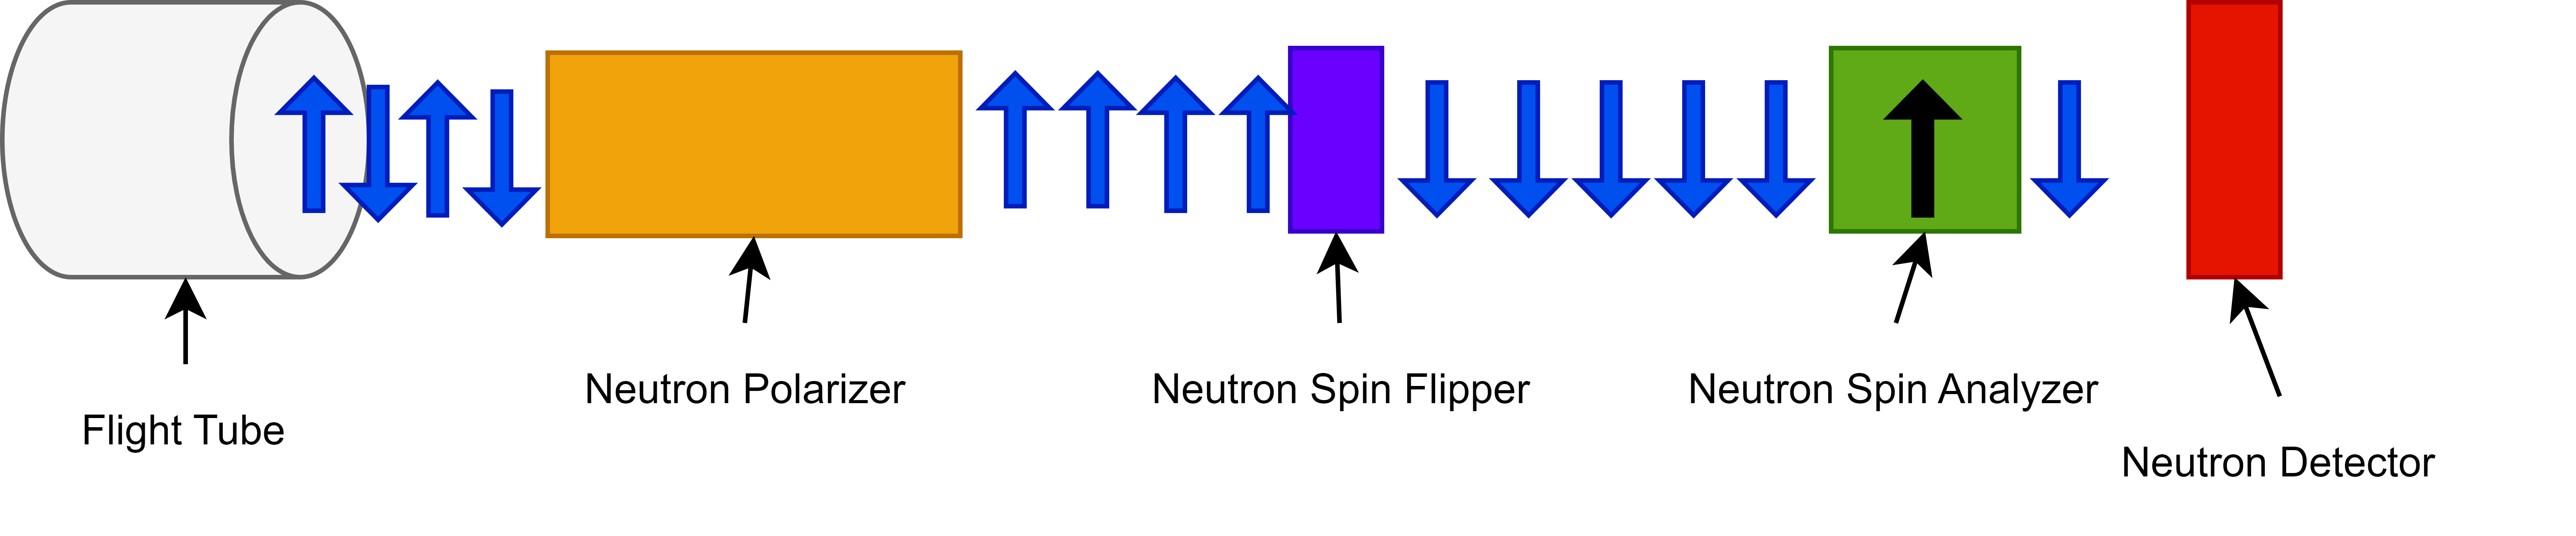
\includegraphics[width=\linewidth, height=2.5cm]{figures/chapter4-figs/sfbeam_polcell.png}
    \caption{$T_{SF}$}
    \label{fig:sfbeam_polcell}
    \end{subfigure}

    \begin{subfigure}[b]{0.75\linewidth}
        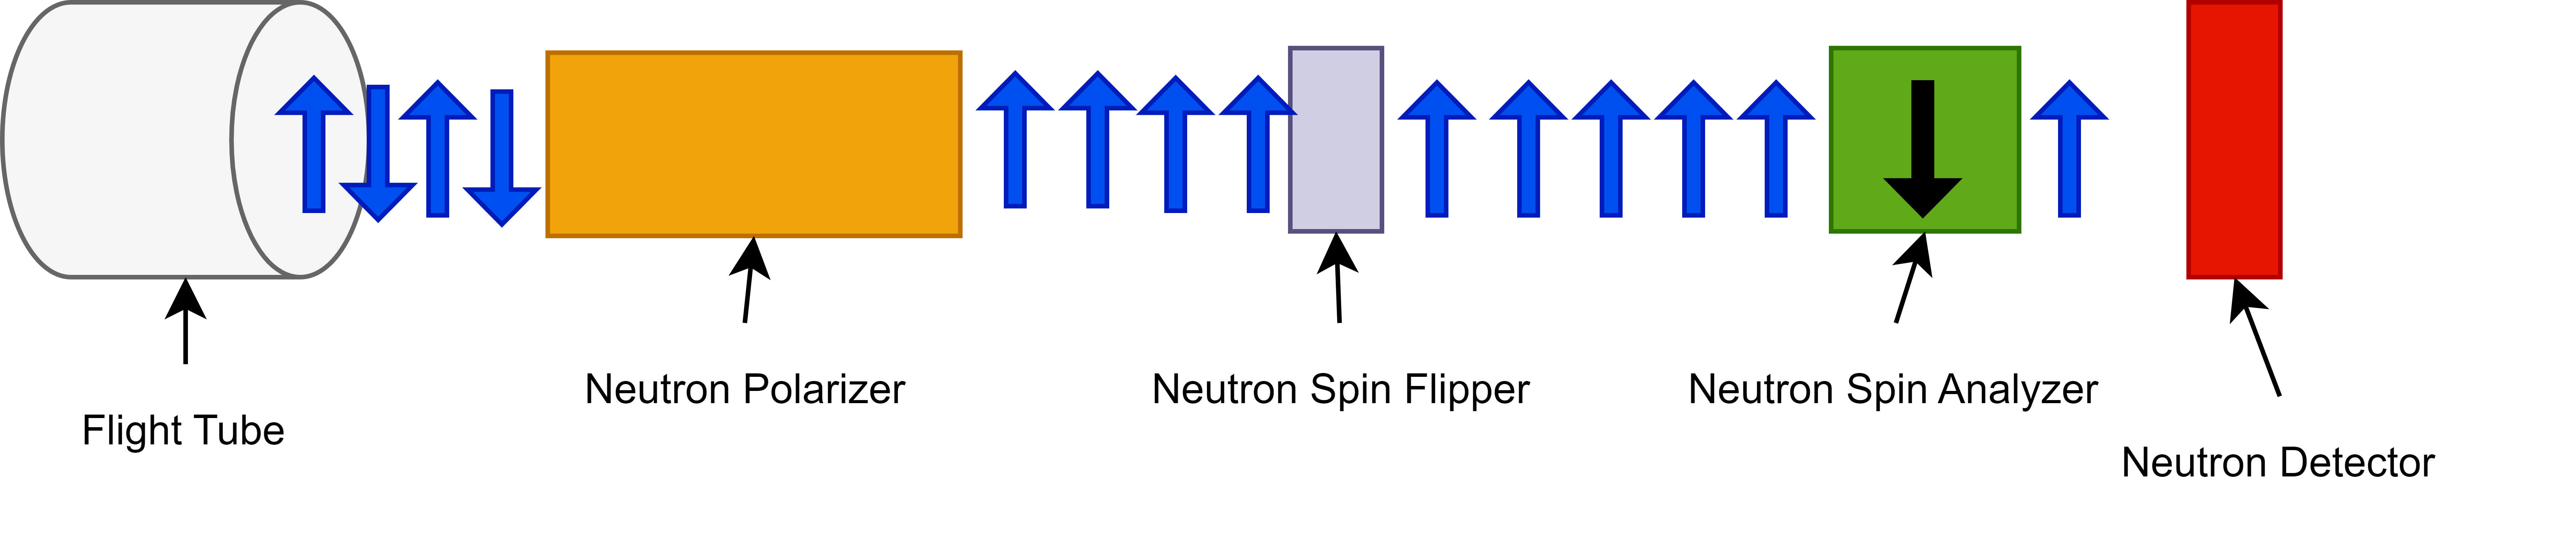
\includegraphics[width=\linewidth, height=2.5cm]{figures/chapter4-figs/polbeam_afpcell.png}
    \caption{$T^{AFP}$}
    \label{fig:polbeam_afpcell}
    \end{subfigure}
    \hfil
    \begin{subfigure}[b]{0.75\linewidth}
        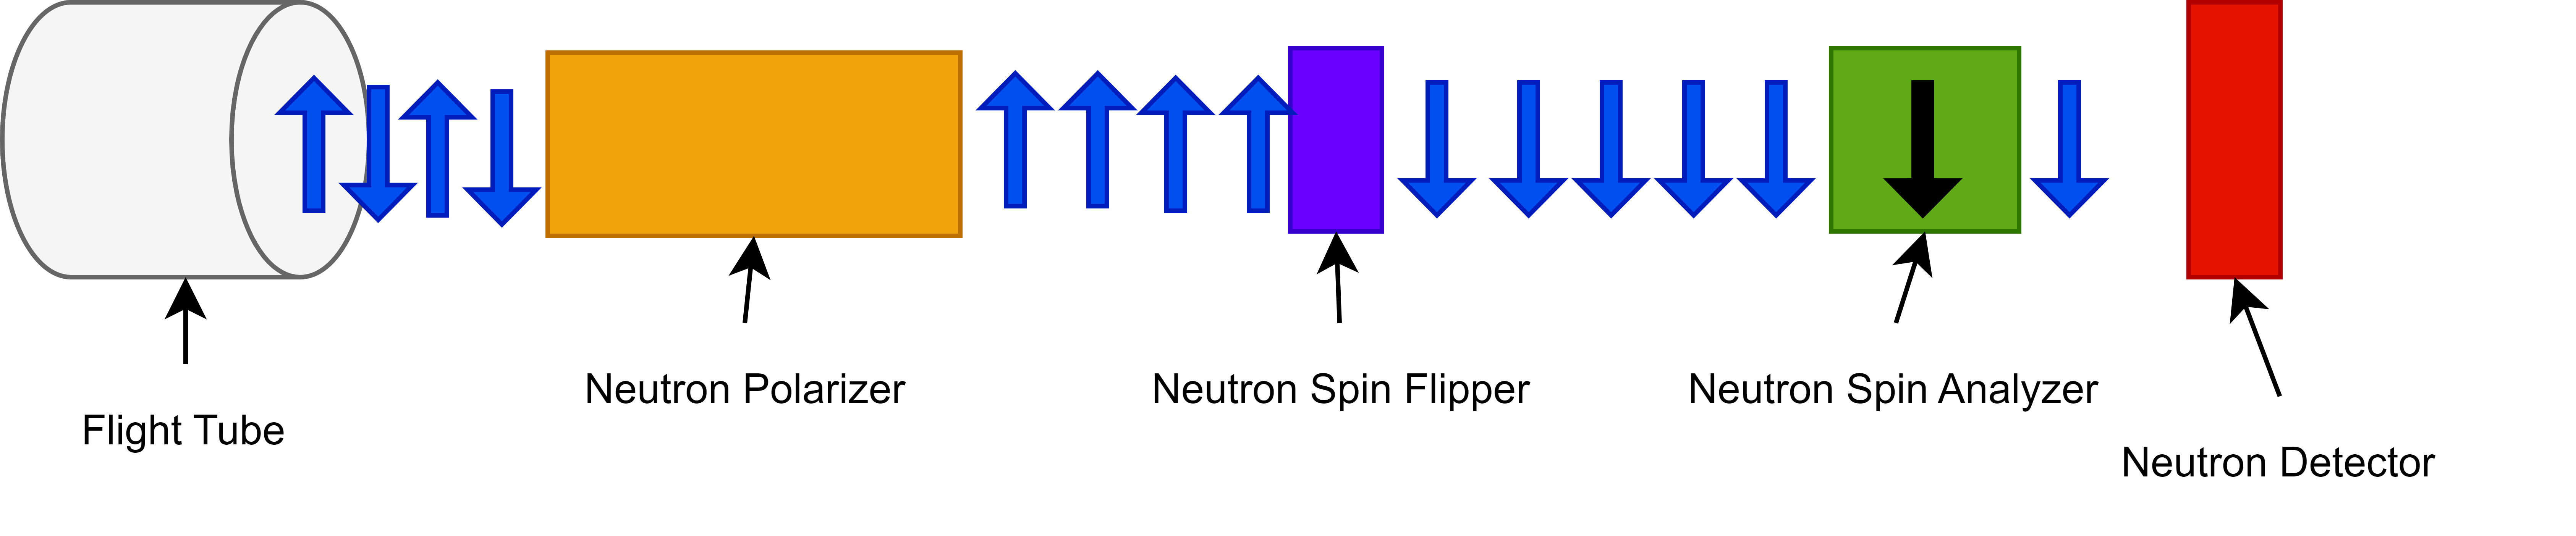
\includegraphics[width=\linewidth, height=2.5cm]{figures/chapter4-figs/sfbeam_afpcell.png}
    \caption{$T^{AFP}_{SF}$}
    \label{fig:sfbeam_afpcell}
    \end{subfigure}
\caption{Transmission of polarized neutrons through $^3$He cell for neutron polarimetry.}
\label{fig:pol_scheme}
\end{figure}
\clearpage}


\subsection{Neutron Polarizer}

Due to their nuclear potential and the magnetic moment, neutrons are capable of coherent nuclear scattering as well as magnetic scattering of off materials or a mirror coated with a magnetizable layer \cite{Hughes1951}. The nuclear and magnetic scattering lengths, $a_{nuc}$ and $a_{mag}$, respectively, of these mirrors make up the neutron’s index of refraction , $n$, as:
\begin{equation}
    n \simeq 1- \frac{N \lambda^2}{2 \pi} \left( a_{nuc} \pm a_{mag} \right)
\end{equation}
where $N$ is the atomic number density of mirror and $\lambda$ is the incident neutron wavelength. The mirror is placed in a polarization defining magnetic field from which the difference in the magnetic scattering length arises, leading to a reflection/refraction of neutron spin states \cite{Hughes1951, Scharpf1991}. From Snell's law, the critical angle of the spin dependent neutron reflection/refraction can be written as:
\begin{equation}
    \theta_c = \lambda \sqrt{  \frac{N}{\pi}  \left( a_{nuc} \pm a_{mag} \right) }
    \label{eq:critangle}
\end{equation}
Between the two critical angles formed by \cref{eq:critangle}, the neutrons are effectively polarized, where one spin state is reflected and the other is refracted i.e. transmitted through the mirror \cite{Hughes1951, Scharpf1991}. 

The critical angle range can be extended to allow for large angle of incidence acceptance and polychromatic neutron beams by employing "super mirrors" \cite{Mezei1976, Mezei1977}. The super mirror is composed of multiple layers of non-magnetic/magnetic bi-layer mirrors. By layering a magnetic material with large nuclear and magnetic scattering lengths with a nonmagnetic material with a scattering length close to zero, a neutron polarizing mirror is created that is highly reflective for one spin state. If the nuclear and magnetic scattering lengths of the magnetic material are approximately equal, the scattering length is constant and close to zero for the other spin state. The supermirror multi-layers vary in thickness to create virtual lattices of different spacings, allowing for multiple Bragg reflections for multiple wavelengths of neutrons, effectively increasing the supermirror’s reflectivity beyond the critical angle of the magnetized bi-layers \cite{Mezei1976, Mezei1977}. This makes super mirrors useful for polarizing a broad range of neutron wavelengths. The reflectivity is constant for incidence angles less than the critical angle of the magnetic material. Beyond that, the reflectivity declines until the effective critical angle created by the super mirrors. This effective critical angle is characterized by the ``$m$" factor. The $m$ factor is relative to the neutron reflection off a $^{58}$Ni surface, since $^{58}$Ni has the largest single layer critical angle. Thus, the $m$ factor indicates that the supermirror’s critical angle is a factor of $m$ greater than a smooth $^{58}$Ni surface and can be found from:
\begin{equation}
   \theta_{c,smp}[mrad] =1.73 \left[\frac{mrad}{\AA} \right] \cdot \lambda [\AA] \cdot m 
\end{equation}
 
This polarization and transmission measurement utilized a 40~cm long and 10~cm $\times$ 12~cm supermirror polarizer, composed of 45 panes (each 0.3~mm thick) of borofloat glass with Fe/Si coating of m=3 \cite{Balascuta2012}, to polarize the monochromatic neutron beam. The panes have a 9.6 cm radius of curvature to (i) accept the divergence of the incoming beam and (ii) to ensure the incoming neutrons experience at least a single bounce and hence, polarize before emerging from the instrument. Iron is used for the ferro-magnetized layers, and Silicon forms the magnetically transparent layers due to it's small neutron scattering cross section \cite{Balascuta2012, Schanzer2016}. Permanent magnets envelop the supermirror polarizer and create a magnetic field of about 380 Gauss to saturate the magnetization of the Fe layers \cite{Balascuta2012}. The magnetization Fe layers create the magnetic scattering length for the supermirror polarizer \cite{Schanzer2016, Mezei1976}. The neutrons with angle of incidence greater than the $\theta_{c,smp}$ refract into the borofloat substrate and get absorbed while the neutrons with glancing angle reflection emerge from the SMP as polarized \cite{Balascuta2012}. Since the polarization from the supermirror depends on the wavelength and angle of incident of the neutron beam and is time-independent, the polarization of the neutron beam does not have to be continuously measured for each neutron pulse. %About 95 $\%$ polarization is expected from the supermirror polarizer for neutron wavelengths 8.9 \AA.

The controlling parameter of the supermirror polarizer is its alignment with the neutron beam. A rough translational as well as rotational alignment was performed to ensure the logitudinal axis of the polarizer was parallel to the beam axis of the flight tube. The important rotation angle to consider is the rotation about the yaw axis at the pivot of the upstream end of the polarizer with respect to the beam. McStas simulations of the polarizer, as shown in \cref{fig:mcstas_pol_sweep}, show the that maximum transmission of neutrons from the polarizer occurs the yaw angle of $0 \degree$. The polarizer was set to this angle for all the measurements taken. Technically, the figure to tune the ideal yaw angle of the polarizer is $P \cdot T^2$, where, $P$, is the neutron polarization and, $T$, is the neutron transmission. However, it can be argued because the design of the polarizer prohibits line of sight neutrons, all neutrons exiting the polarizer have had a chance to bounce of the supermirror surface and hence, become polarized. Therefore, it was sufficient to use the maximum transmission setting as the ideal.  

\afterpage{
\begin{figure}
    \centering
    \includegraphics[width=\textwidth]{figures/chapter4-figs/pol_rot.png}
    \caption{McStas simulated neutron intensity transmitted from the supermirror polarizer as a function of the yaw angle about the vertical axis.}
    \label{fig:mcstas_pol_sweep}
\end{figure}
\clearpage}

%For most materials, which possess neutron refractive indices slightly smaller than 1, neutrons will undergo total external reflection from the optical potential $V_{opt}$ of the medium if their angle of incidence is below a critical angle ${\theta}_c$, determined by the material density, the neutron coherent scattering length $b_{coh}$, and the neutron wavelength.
%\begin{equation}
    %\theta_c=\lambda\sqrt{\frac{Nb_{coh}}{\pi}}
%\end{equation}
%where reflection of neutrons with wavelengths beyond the critical angle is achieved by layering materials with different refractive indices to simulate a virtual one-dimensional lattice of spacing d for Bragg diffraction [7].
%\begin{equation}
 %   n\lambda=2d\sin{\theta}
%\end{equation}

%A neutron entering a medium will interact with its nuclear potential. The low energy neutrons being utilized for this experiment have kinetic energies of $\sim$1 meV, ($\lambda_n \sim nm$) which is much less than the typical nuclear potential of tens of MeV with only a couple of femtometer range. This means that wavelength of these low energy neutrons is much longer compared to the range of the nuclear potential. If we assume that the neutron experiences a change of energy equivalent to the effective potential of the entire medium, $\langle V \rangle$, the index of refraction can be written as:

\subsection{Spin Flipper}

The polarization direction of the neutron beam is defined by the guiding magnetic field. This guiding magnetic field can be adiabatically reoriented and hence, in the lab frame, the polarization of the beam with respect to the guide field will remain constant, following the adiabatically reoriented guiding magnetic field. However, for a diabatic reorientation of the guiding magnetic field, the polarization will not follow the sudden change in the guiding magnetic field direction; instead the neutron beam will preserve its initial state, and precess about the new guiding magnetic field direction. These adiabatic and diabatic rotations of the guiding magnetic field enable the neutron beam polarization to be effectively inverted or flipped with respect to the guiding magnetic field. 

In order to determine the neutron beam polarization, the neutron spin state anti parallel to the guide field also has to be characterized, since polarization is defined as the contrast in parallel and anti-parallel spin states. In order to  measure the transmission of spin flipped neutrons through the analyzer cell, $T_{sf}$, a neutron spin flipper is used to flip the neutron spin to the opposite spin state. Since this experiment is dealing with monochromatic neutrons, i.e. neutrons of fixed velocity, diabatic spin flippers are appropriate. A Mezei coil is a type of a diabatic flipper that was built for this purpose \cite{Mezei1972, Hayter1978}. This flipper consists of a rectangular solenoid of fixed thickness, which provides a strong DC magnetic field perpendicular the guide field to induce a torque on the magnetic moment of the polarized neutrons of fixed velocity for $n\pi$ radians spin flips, where n is an odd integer. The strength of the perpendicular flipper field, $B_{flipper}$, can be found by:
\begin{equation}
    \gamma_n B_{flipper} = \frac{\phi v_n}{ d}
\end{equation}
where $\phi$ is the spin rotation angle, $v_n$ is the velocity of the neutrons, $d$ is the thickness of the coil and $\gamma_n$ is the neutron's gyromagnetic ratio.

A Mezei spin flipper was constructed to be used for this experiment, as shown in \cref{fig:Mezei-built}. The flipper consists of four major parts: (i) The inner most coil, made of Aluminum ribbon wire, is the spin flip coil responsible for providing the perpendicular guide field, (ii) The outer frame of the flipper is responsible for providing a continuous guide field. Permanent magnets are placed on the sides and the iron yokes provide a homogeneous field return, (iii) the outer most coil, also made of aluminum ribbon wire, cancels the guide field, so that the neutron effectively precesses about the perpendicular field created by (i). The neutron beam goes through middle of the coil. There are two pairs of orthogonal shim coils that can provide a cancelling field in the beam axis, if needed.

\afterpage{
\begin{figure}
    \centering
    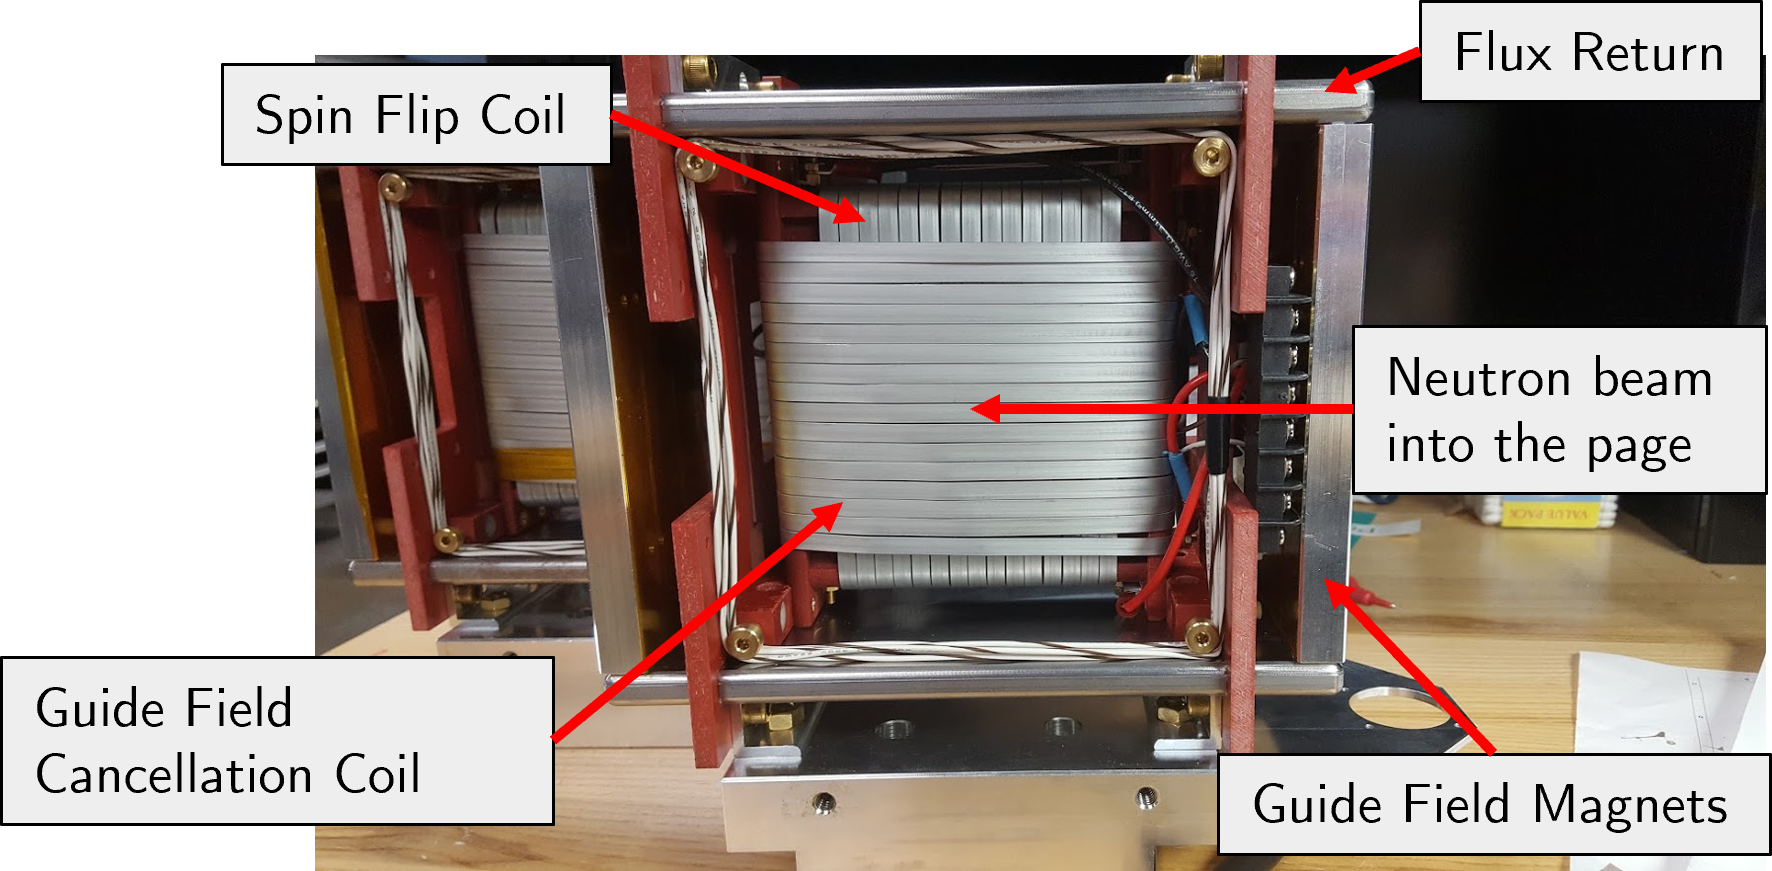
\includegraphics[width=\textwidth]{figures/chapter4-figs/Flipper_picture.png}
    \caption{The Mezei spin flipper built for the neutron polarimetry and transmission experiment.}
    \label{fig:Mezei-built}
\end{figure}
\clearpage}

\afterpage{
\begin{figure}
    \centering
    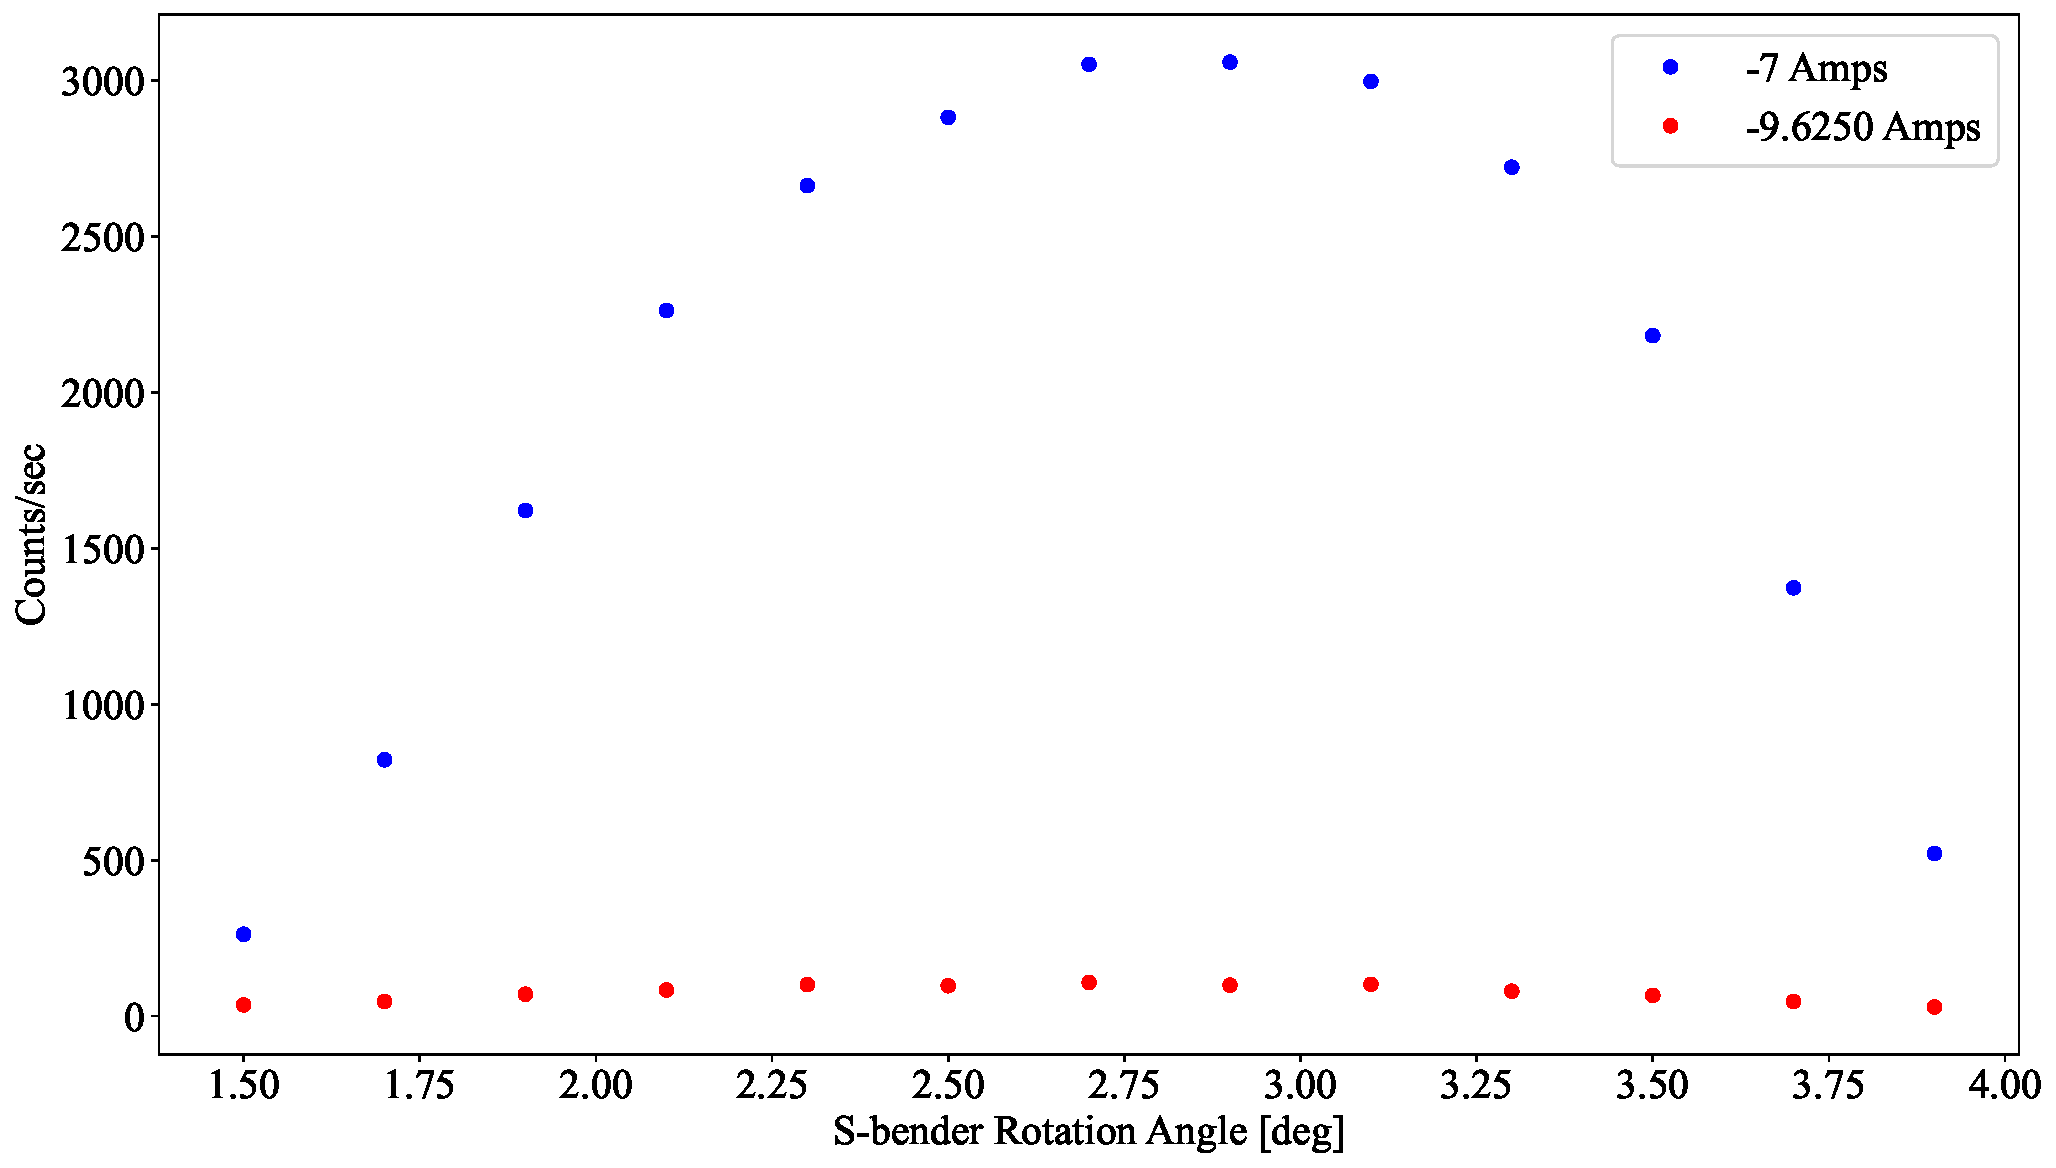
\includegraphics[width=\textwidth]{figures/chapter4-figs/HB2D_Sbender.pdf}
    \caption{4.2~\AA\ neutron count rate while sweeping the S-bender angle.}
    \label{fig:benderopt_HFIR}
\end{figure}
\clearpage}

\afterpage{
\begin{figure}
    \centering
    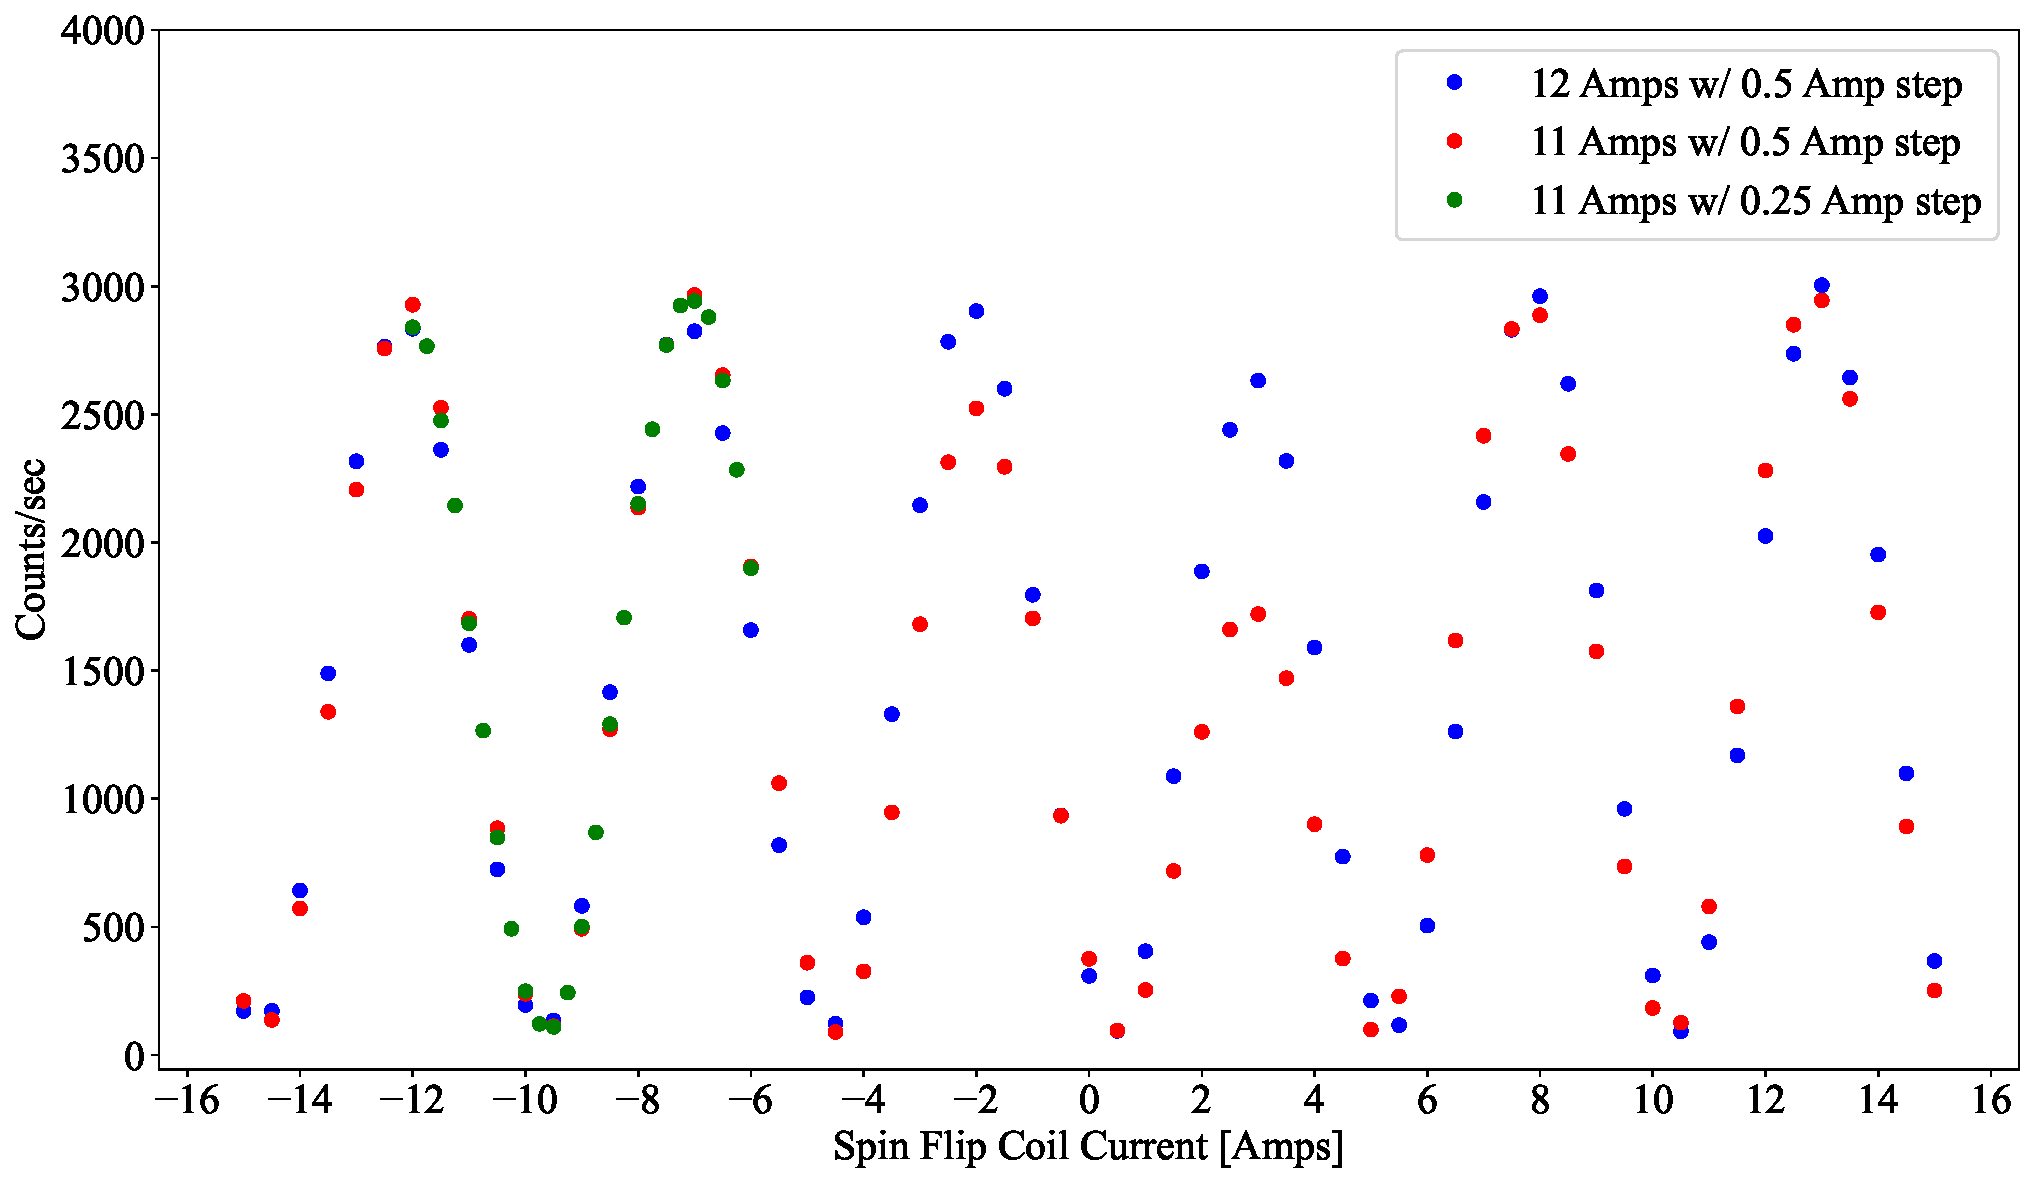
\includegraphics[width=\textwidth]{figures/chapter4-figs/HB2D_SFtest.pdf}
    \caption{4.2~\AA\ neutron count rate at 2.6$\degree$ S-bender angle while sweeping the flipper coil current for different guide field cancellation coil currents.}
    \label{fig:SFeff_HFIR}
\end{figure}
\clearpage}

This flipper was tested at the HFIR neutron instrument developed beamline (HB2D), which is designed for testing prototypes of neutron polarizing devices \cite{Crow2016}. HB2D consists of a monochromatic 4.2~\AA\ neutron beam, a V-cavity neutron polarizer, a S-shaped bender polarizer \footnote{See \href{https://www.swissneutronics.ch/}{SwissNeutronics} for more information on the different types of neutron devices.} for neutron spin analysis and a $^3$He detector for neutron counting \cite{Crow2016}. The test included characterization of the flipping ratio and hence, the flipping efficiency of Mezei flipper based on the methodology described in \cite{Li2020, Dadisman2020}, where RF and adiabatic neutron spin flippers were characterized similarly at HB2D. The transmission measurements of polarized neutrons through the Mezei spin flipper as a function of flipper coil current were preformed. First, the S-shaped bender polarized neutron analyzer was optimized by measuring the transmission of polarized neutrons as a function of the angle of incidence of the incident neutron beam. The results are shown in \cref{fig:benderopt_HFIR}. The S-bender analyzer was set at the optimum angle of $2.6\degree$ for the flipper testing. Next, the flipper was optimized by varying the spin flipper coil current for different current values of the guide field cancelling coil. \cref{fig:SFeff_HFIR} shows the the high transmission spin state neutrons (based on the S-bender spin selection preference) and low transmission spin state neutrons as a sweep of the spin flipper current coil. The best flipping ratio, $f=\frac{N_{high}}{N_{low}}$, or the spin contrast was measured as 26.74 at 9.8 A current in the spin flipper coil. The polarizing efficiency of the spin flipper, $\frac{f-1}{f+1}$, at 4.2~\AA\ was measured as:
\begin{equation}
    \epsilon_{SF} = 0.93 \pm 0.06_{stat}
\end{equation}
This measurement was repeated for 8.9~\AA\ neutrons at beamline 13A. First, the outer coil current was swept with no spin flip coil current to find the lowest transmission of neutrons. This occurred at an outer coil current of -17.5 A, indicating that at this current value, the outer coil was maximally cancelling out the guide field and causing a diabatic transmission. Next, the spin flipper coil current was swept to find the maximum flipping ratio. The results are shown in \cref{fig:SFeff_SNS}, where the maximum flipping ratio of $\approx1.7$ took place at -5.8 A. The flipping efficiency at 8.9~\AA\ was measured to be:
\begin{equation}
    \epsilon_{SF} = 0.92 \pm 0.03_{stat}
\end{equation}
Two important observation should be noted here. First, both \cref{fig:SFeff_HFIR} and \cref{fig:SFeff_SNS} show that that spin flipping contrast is more robust at higher currents i.e. large $B_{flipper}$, meaning the effective magnetic field from the flipper coils becomes more and more perpendicular. Therefore, it is more efficient to use $3\pi, 5\pi, ...$ and beyond spin turns for more robust spin flips. Second, the fringe pattern observed for 4.2~\AA\ neutrons in \cref{fig:SFeff_HFIR} is twice as broad as the pattern observed for 8.9~\AA\ neutrons in \cref{fig:SFeff_SNS}. This is because 4.2~\AA\ are faster than 8.9~\AA\ neutrons and therefore, a high $B_{flipper}$ field i.e. high coil current, is needed to provide a torque to flip their polarization. 

\afterpage{
\begin{figure}
    \centering
    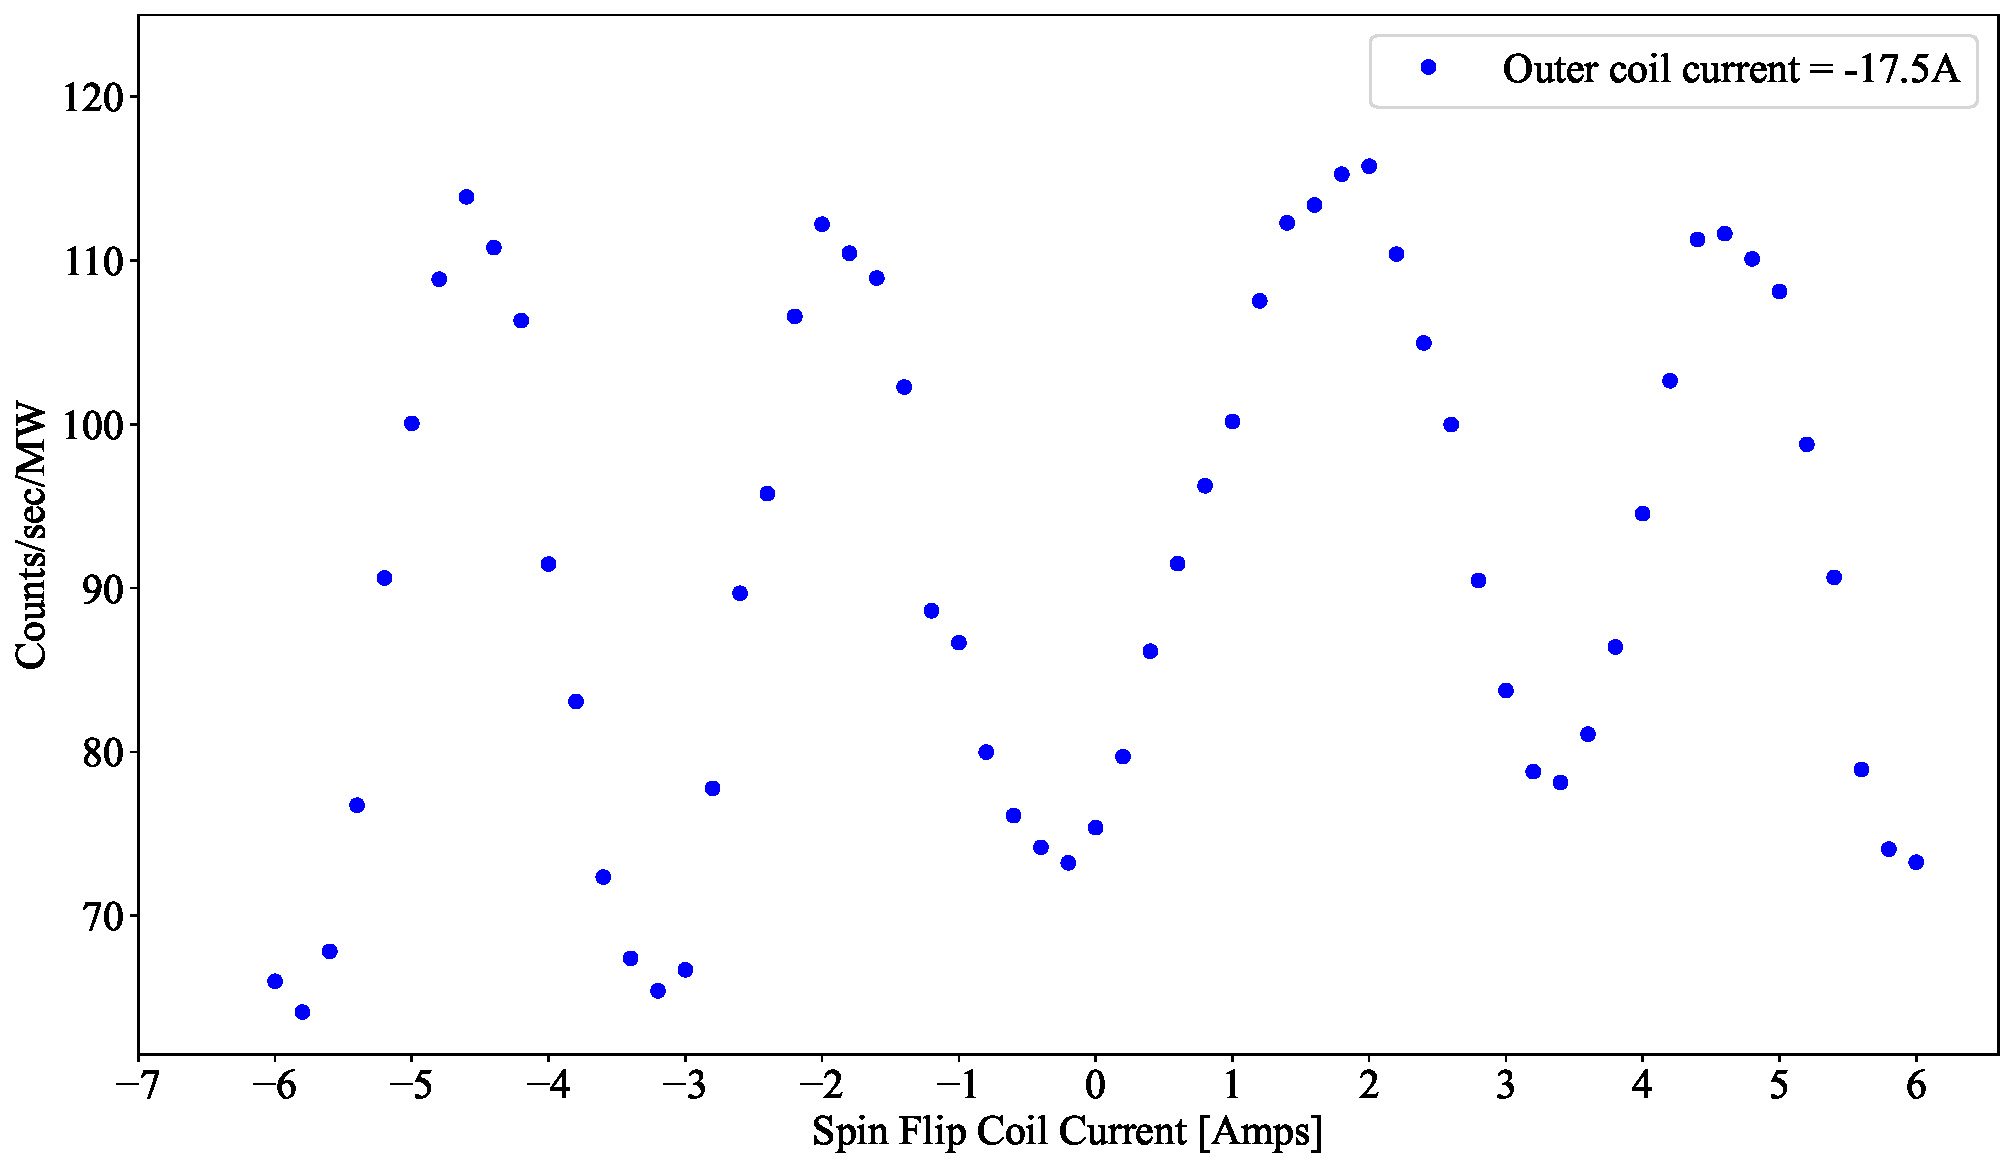
\includegraphics[width=\textwidth]{figures/chapter4-figs/SNS_SFtest.pdf}
    \caption{8.9~\AA\ neutron count rate while sweeping the flipper coil current for the guide field cancellation coil current of -17.5 A.}
    \label{fig:SFeff_SNS}
\end{figure}
\clearpage}

\subsection{Neutron Spin Transport}

To describe the polarization of the neutron beam, a semi-classical picture is used, where a neutron with a magnetic moment aligned with the spin angular momentum vector, $\Vec{S}$, precesses in a magnetic field, $\Vec{B}$, with an angular frequency, $\omega_L$, called Larmor frequency defined as $\omega_L$ = $\gamma_n \Vec{B}$. The rate of change of the angular rotation of the spin (under cartesian coordinates) is given by the Bloch equation\cite{Bloch1946}:
\begin{equation}
    \frac{d\Vec{S}(t)}{dt} = \gamma_n \left( \Vec{S}(t) \times \Vec{B}(t)  \right)
    \label{eq:Bloch}
\end{equation}
which when written in terms of all of the components of $\Vec{S}(t)$ and $\Vec{B}(t)$ becomes:
\begin{align}
\begin{split}
    \frac{dS_x(t)}{dt} &= \gamma_n \left( S_y(t) B_z(t) - S_z(t) B_y(t) \right) \\
    \frac{dS_y(t)}{dt} &= \gamma_n \left( S_z(t) B_x(t) - S_x(t) B_z(t) \right) \\
    \frac{dS_z(t)}{dt} &= \gamma_n \left( S_x(t) B_y(t) - S_y(t) B_x(t) \right)
    \label{eq:Blochcomp}
\end{split}
\end{align}
The time evolution of \cref{eq:Blochcomp} can be written in terms of the ratio of the distance travelled by the neutron in the guiding magnetic field, $l$, to the velocity of the neutron, $v_n$. This means that, \cref{eq:Blochcomp} can be used to trace the dynamics of the spin vector components of a neutron propagating through an arbitrary magnetic field environment over the course of the experimental setup. Using this technique, the spin transport for the monochromatic 8.9~\AA\ neutrons, i.e. velocity of 444 m/s, was simulated based on the magnetic fields created by the guide field and polarimetry components of the experiment.

\afterpage{
\begin{figure}
    \centering
    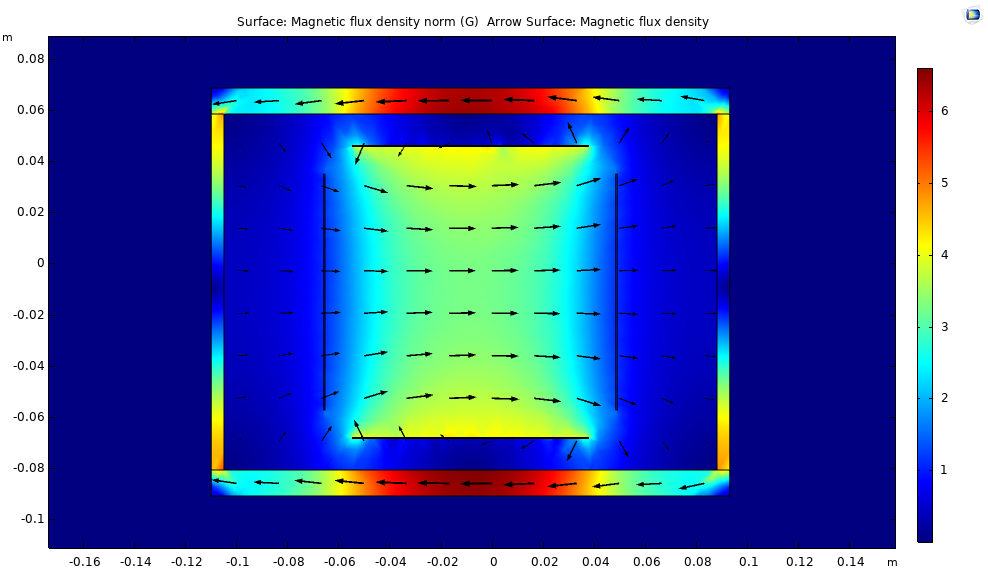
\includegraphics[width=1\textwidth]{spinflipper2.png}
    \caption{A simulation of the magnetic field profile of diabatic spin flipper. The neutron beam direction is into/out of the page. The color gradient shows the magnitude of magnetic flux density [Gauss] and the arrows show the direction of magnetic flux density.}
    \label{fig:spinflipper_field}
\end{figure}
\clearpage}

The magnetic field from the guide field components as well as the polarimetry components were modeled in COMSOL Multiphysics \cite{COMSOL2019}, a finite element software for AC/DC electromagnetics. A rendition of the geometry of the key components and their current sources with the boundary conditions was built and magnetic field profile was simulated. Since, the neutron beam gets polarized in the polarizer, it is only relevant to simulate the magnetic fields, which will be experienced by the neutron beam following the polarizer. The polarizer's fringe field was reproduced via a polynomial fit on the measured polarizer fringe fields from \cite{Balascuta2012}. The Mezei flipper geometry was built and based on the expected current settings, its magnetic field profile was simulated as shown in \cref{fig:spinflipper_field}. Another guide field component, called the neutator\footnote{Neutator is short for neutron guide field rotator.} was also employed. The purpose of the neutator is provide a continuous guide field, remove any magnetic field zero crossing and in the case of this experiment provide an adiabatic rotation of the spin to match the magnetic field inside the cryogenic magnet as well as the in situ $^3$He polarizer. \Cref{fig:nutator} shows the simulation of magnetic fields produced by a neutron guide field component. The magnetostatic cavity of the in situ $^3$He system was also simulated and the resulting magnetic field profile is shown in \cref{fig:nutatormerritt}. The full magnetic field profile of the experimental setup is shown in \cref{fig:upstreambfield} for the cryomagnet upstream polarimetry and guide field components and \cref{fig:downstreambfield} for the cryomagnet downstream polarimetry and guide field components. 

The simulated magnetic field profiles from these components were used to trace the spin dynamics of the polarized neutron beam. A numerical solver for \cref{eq:Blochcomp} was developed using the adaptive \texttt{RKDP45} method \cite{Dormand1980} to perform a check for the adiabatic transport of neutrons and identify any magnetic field zero crossings. For these simulations, the initial spin was biased to $S_y$, indicating a fully polarized beam exiting the polarizer. Spin relaxation was not included in these simulations because of lack of knowledge of any possible background fields. \Cref{fig:upstreamspin} shows the simulated components of the spin vector interacting with the magnetic field profile of the upstream components shown \cref{fig:upstreambfield}. The polarized beam gets spin flipped by the diabatic flipper as the $S_y$ flips to $-S_y$. The polarization is then preserved as it goes through three guide fields and then gets adiabatically rotated to the $x$ direction by the neutator. \Cref{fig:downstreamspin} shows the simulated components of the spin vector interacting with the magnetic field profile of the downstream components shown \cref{fig:upstreambfield}. The initial neutron spin is set to $S_x$, to mimic the spin emerging from the cryogenic magnet. The spin gets adiabatically rotated by the neutator and the magnetostatic cavity of the in situ $^3$He polarizer. 

\afterpage{
\begin{figure}
    \centering
    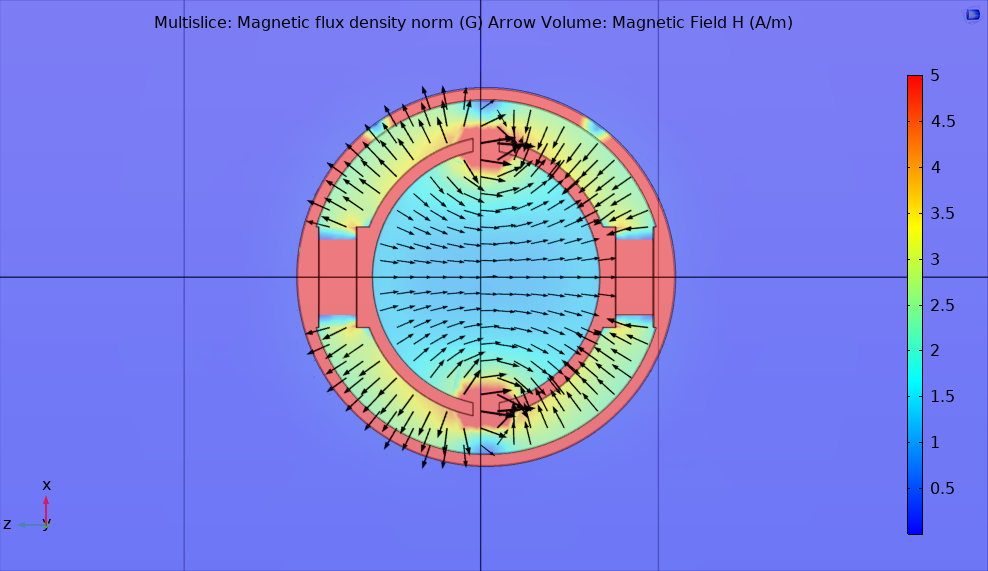
\includegraphics[width=1\textwidth]{Nutator_uniformfield.png}
    \caption{A simulation of the magnetic field profile of the neutron rotatable guide field component. The neutron beam direction is into/out of the page. The color gradient shows the magnitude of magnetic flux density [Gauss] and the arrows show the direction of magnetic flux density.}
    \label{fig:nutator}
\end{figure}
\clearpage}

\afterpage{
\begin{figure}
\centering
\begin{subfigure}[b]{0.9\textwidth}
   \includegraphics[width=1\linewidth, page=3]{figures/chapter4-figs/spin_precession_0cm_vert.pdf}
   \caption{}
   \label{fig:upstreambfield} 
\end{subfigure}

\begin{subfigure}[b]{0.9\textwidth}
   \includegraphics[width=1\linewidth, page=2]{figures/chapter4-figs/spin_precession_0cm_vert.pdf}
   \caption{}
   \label{fig:upstreamspin}
\end{subfigure}

\caption{A magnetic field profile (a) and the subsequent spin precession (b) simulation of 8.9\AA neutrons for the upstream components of neutron polarizer, neutron spin flipper and neutron guide field components. The $x$ direction is the horizontal direction (left-right), $y$ direction is the vertical direction (top-down) and $z$ direction is the beam axis.}
\end{figure}
\clearpage}

\afterpage{
\begin{figure}
    \centering
    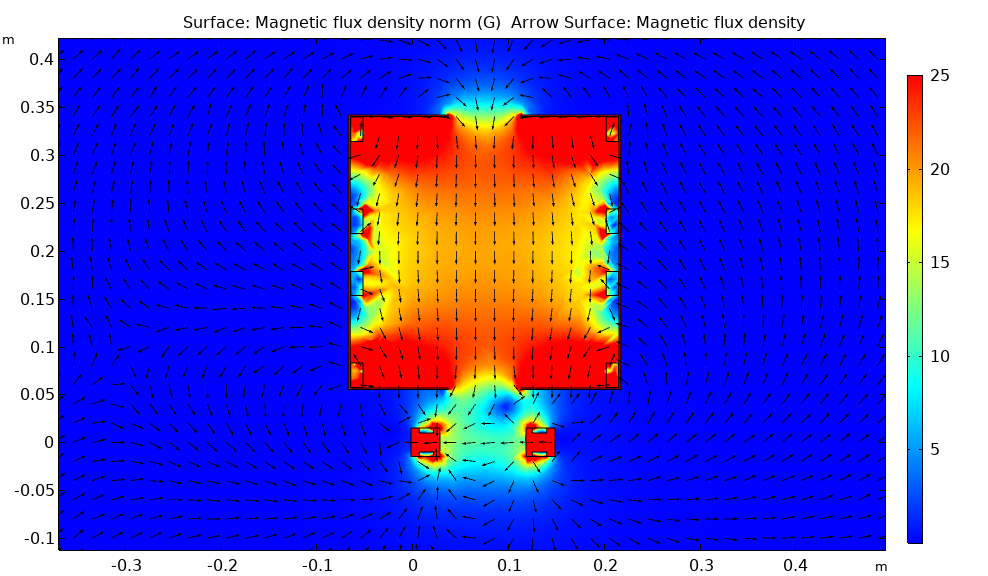
\includegraphics[width=1\textwidth]{nutator_mumetal_bfield.png}
    \caption{A top down view of neutron guide field components and $^3$He spin analyzer holding field coils. The beam direction is vertical direction. The color gradient shows the magnitude of magnetic flux density [Gauss] and the arrows show the direction of magnetic flux density.}
    \label{fig:nutatormerritt}
\end{figure}
\clearpage }

\afterpage{
\begin{figure}
\centering
\begin{subfigure}[c]{0.9\textwidth}
   \includegraphics[width=0.87\linewidth, page=3]{figures/chapter4-figs/downstream_spin_precession_merritt.pdf}
   \caption{}
   \label{fig:downstreambfield} 
\end{subfigure}

\begin{subfigure}[c]{0.9\textwidth}
   \includegraphics[width=1\linewidth, page=2]{figures/chapter4-figs/downstream_spin_precession_merritt.pdf}
   \caption{}
   \label{fig:downstreamspin}
\end{subfigure}

\caption{A magnetic field profile (a) and the subsequent spin precession (b) simulation of 8.9~\AA\ neutrons for the downstream components of neutron guide field component and polarized $^3$He analyzer holding field. The $x$ direction is the horizontal direction (left-right), $y$ direction is the vertical direction (top-down) and $z$ direction is the beam axis.}
\end{figure}
\clearpage}

\subsection{Neutron Detector}

The detector used for this experiment consists of a linear array of eight individual linear position sensitive detectors (LPSD) \cite{Berry2012, Diawara2023}. These LPSDs were 40.6 cm long and 1.2 cm in diameter, constructed from stainless steel tubing (0.5 mm thick). Each LPSD tube is filled with 10 atm of high purity $^3$He gas for neutron capture, plus a small amount of CO$_2$ and Ar as stopping/quench gases. Each LPSDs had a coaxial electrode geometry and is operated in proportional counting mode. The outer tube of the LPSD is the cathode set at ground potential. A central anode wire, which runs along the LPSD axially, is powered up to high voltage potential. The anode ends are shielded from the cathode with ceramic. The eight pack is oriented horizontally. Due to the linear stacking of the LPSDs, the detection active area can be treated as infinite along the length of the tube but limited by the gaps in between the tubes. This is illustrated in \cref{fig:det_eff_diam}'s efficiency plot. The tube stacking effectively provides an active detector area equivalent to that of a single LPSD. Signal waveform preamplifiers are located at the end of the 8 pack LPSD assembly to extract the position sensitive reading and minimize the capacitive noise. The LPSD tubes as well as the preamplifier electronics were manufactured by GE Reuter-Stokes \cite{Berry2012}. 

Helium-3 filled gas proportional neutron detectors are widely used at the SNS and HFIR neutron instruments, and details of their operating principles are well documented in \cite{Knoll2010, Diawara2023}. These principles will be briefly discussed here for context. Cold neutrons undergo the capture reaction $^3$He(n,p)T with $^3$He nucleus, emitting in opposite directions the products proton, $p$, and triton, $T$. The Q value of this capture reaction is 764 keV, which is distributed as kinetic energy of 191 keV for triton and 573 keV for proton. The decay products deposit their kinetic energy in the detector gas creating electron-ion pairs (the W-value \cite{Bichsel1979} for $^3$He is 41-43 eV/ion-pair, which means around 20000 pairs are produced depending on the gas composition\footnote{GE Reuter-Stokes regard the composition of gas mixtures in their detectors as proprietary information.}). The stopping/quenching gases play a major role here. The stopping power of a proton in 10 atm of $^3$He is around 6 mm \cite{Crawford1992}, a little too large for the less than millimeter positional resolution capability of LPSDs, therefore, the stopping gases reduce the size of the electron–ion charge cloud i.e. the mean free path of the electrons, as well as suppress any radiative losses \cite{Doumas2012}.

These LPSDs were operated in proportional counting mode, relying on the mechanism that charge multiplication in the gas, via an applied potential across the electrodes, remains proportional to the primary ionization charge deposited in the gas \cite{Knoll2010, Diawara2023}. For the cylindrical coaxial electrode geometry of the electrodes, the electric field of $E=V/r \cdot Ln(b/a)$ means the electric field is much larger close to the anode wire \cite{Knoll2010, Diawara2023}. Electrons created from the primary ionization charge drift in this high electric field region, acquiring kinetic energy, and near the anode create a Townsend avalanche \cite{Knoll2010, Diawara2023}. This avalanche charge multiplication, also called the gain, has an $\approx \exp(-V_{applied})$ relation to the applied voltage, meaning a charge of several orders of magnitude greater than the primary charge can be collected by the anode wire \cite{Knoll2010, Diawara2023}. 

The LPSDs in this experiment use the resistive anode charge division technique to locate the neutron interaction along the length of the detector tube \cite{Alberi1977, Radeka1979}. This feature allows for the two dimensional neutron beam profile measurements, albeit limited by the finite width of the LPSDs. The schematic shown in \cref{fig:char_resist} illustrates how neutron detection location is determined. Resistive anode charge division, as the name suggests, employs a uniformly resistive wire as the anode. Based on the location of the neutron interaction point, the relative charge division according to the relative resistances $R_A$ and $R_B$ between the anodes and hence, the current signal between the two ends of the anode is compared. Preamplifiers at each end of the anode convert the divided current signals into voltages $V_A$ and $V_B$. The analog sum of the two voltages is measured against a threshold to determine if the signals represent  a neutron event. If yes, then the asymmetry ratio, $\frac{V_A-V_B}{V_A+V_B}$, determines the interaction location along the tube \footnote{It is possible that the asymmetry can also form based on the difference in the arrival time of the signal created by the trajectory of the neutron capture decay products.}. 

\Cref{fig:PH_spectrum} shows a measured pulse height spectrum from the LPSD taken during a summer 2023 data run. The horizontal axis is the sum of the ADC readings from both sides of the LPSD from a detection event, the range for which the detector is configured is divided into 1024 bins \cite{Beal2021}. The vertical axis is the accumulated counts within a bin size of one ADC step during the acquisition. For the neutron proportional counters, the neutron capture reaction, regardless of the incident neutron energy, is always based on the Q-value which occurs at the same energy. It is better to interpret the pulse-height spectrum as an indicator of any variation in the amount of charge collected from neutron capture events \cite{Diawara2023}. A threshold of 200 ADC units was set to discriminate the signals from the noise. Events beyond the 200 ADC were considered as event from a neutron capture in the tubes.

\afterpage{
\begin{figure}
    \centering
    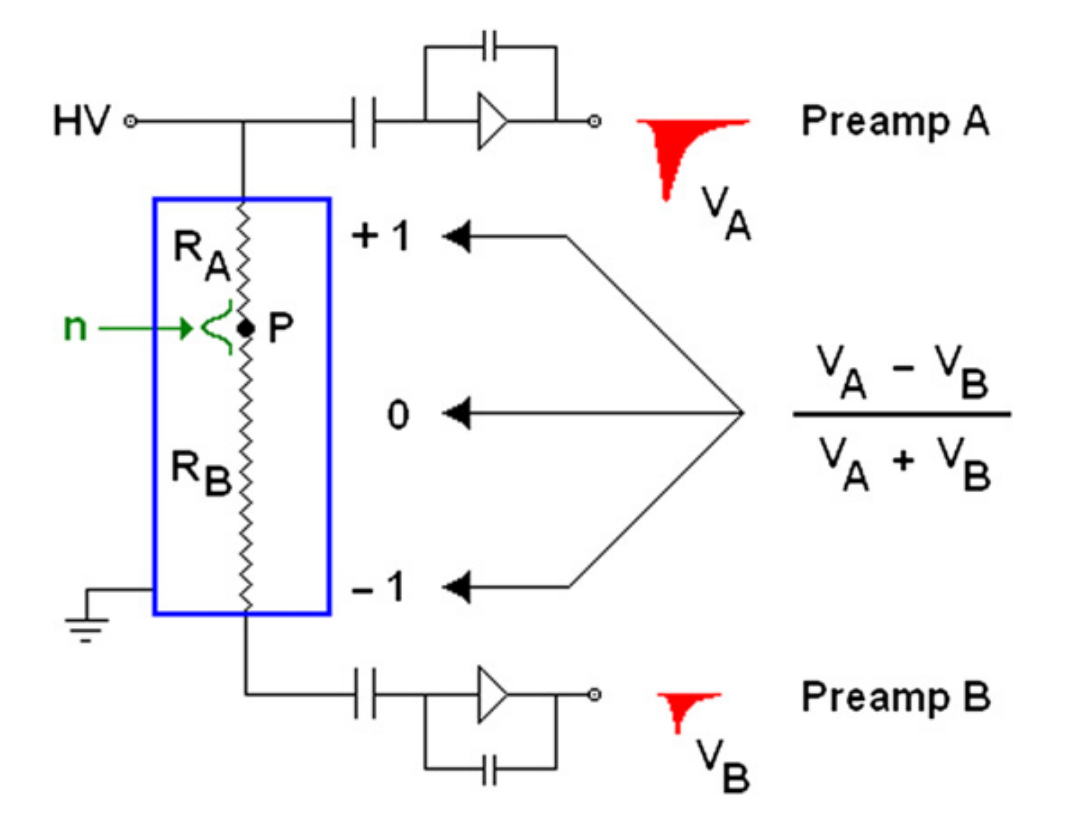
\includegraphics[width=\textwidth]{figures/chapter4-figs/chargeresistivepic.png}
    \caption[A schematic diagram showing the neutron position sensitivity feature of the LPSD based on the resistive charge division technique.]{A schematic diagram showing the neutron position sensitivity feature of the LPSD based on the resistive charge division technique. Figure is taken from \cite{Berry2012}.}
    \label{fig:char_resist}
\end{figure}


\begin{figure}
    \centering
    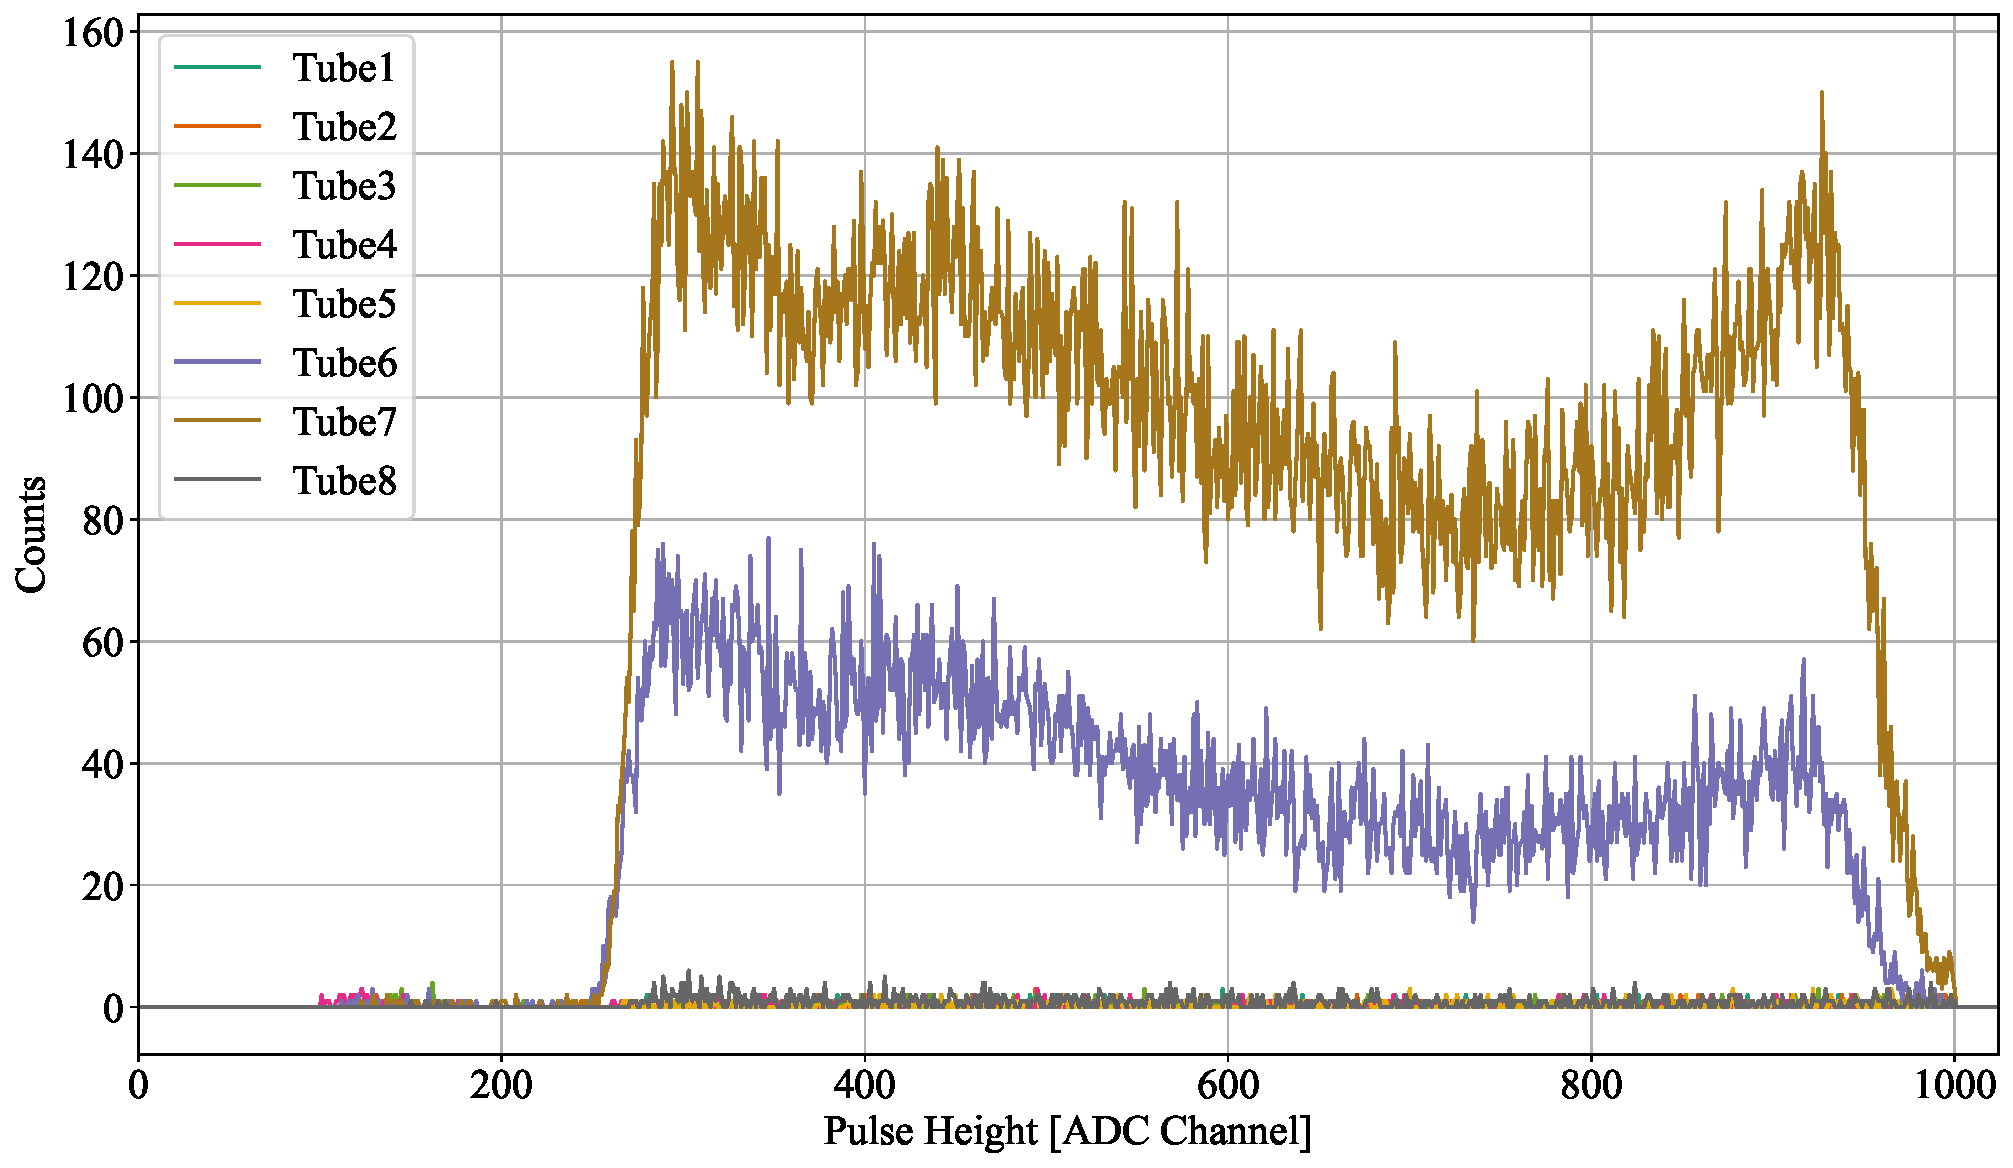
\includegraphics[width=\textwidth]{figures/chapter4-figs/trans_det_up_PH.pdf}
    \caption{A pulse height spectrum of the 8.9~\AA\ neutrons incident on the LPSDs. A 1 cm by 1 cm aperture was in place before the LPSD, therefore, only two tubes out of the eight were active.}
    \label{fig:PH_spectrum}
\end{figure}
\clearpage}

Dead time inefficiency from high count rates can prove a limitation for LPSDs and have to be understood to verify their applicability. There is about a 1$\mu s$ dead time when the charge from an event is integrated. High count rates can lead to a dead time if the integrator has not yet reset from first event integration, increasing the fraction of vetoed events. This can lead to a skewed position hit determination along the LPSD. The increased levels of ionization in the tube from high count rates can lead to charge saturation, limiting the amount of charge collected, leading to under counting. Previous studies have shown that these effects are negligible up until 100 kHz instantaneous neutron beam \cite{Diawara2023}.

Neutrons incident on the LPSDs will attenuate along the diameter as $ I = I_0 \exp(-\sigma \cdot N \cdot P \cdot d) $, where $I$ are the attenuated neutrons, $I_0$ are the incident neutrons, $\sigma$ is wavelength dependent absorption cross section in cm$^2$, N is the $^3$He number density [$2.7 \times 10^{19}$ atoms cm$^{-3}$ atm$^{-1}$], P is the gas pressure [10 atm] and $d$ is the tube thickness [1.2 cm]. The fraction of the beam detected by the gas, or in other words, the capture efficiency is given by:
\begin{equation}
    \epsilon = 1 - \frac{I}{I_0} = 1 - \exp \left( - \sigma(\lambda_n) \cdot N \cdot P \cdot d \right)
\end{equation}
Shorter wavelength neutrons will penetrate more deeply as compared to longer wavelength neutrons. This may result in some wavelength dependence on the amount of charge collected \cite{Diawara2023}. If the neutron’s trajectory is not at normal incidence to the tube, the penetration depth can also influence the capture efficiency. \Cref{fig:det_eff_wave} shows the detector capture efficiency of unity for 8.9~\AA\ incident neutron beam. \Cref{fig:det_eff_diam} shows a single LPSD tube efficiency of unity except for near the edges of the tube, meaning there were dead zones in between tubes, but minimal.

\afterpage{
\begin{figure}
\centering
    \begin{subfigure}[b]{0.475\textwidth}
    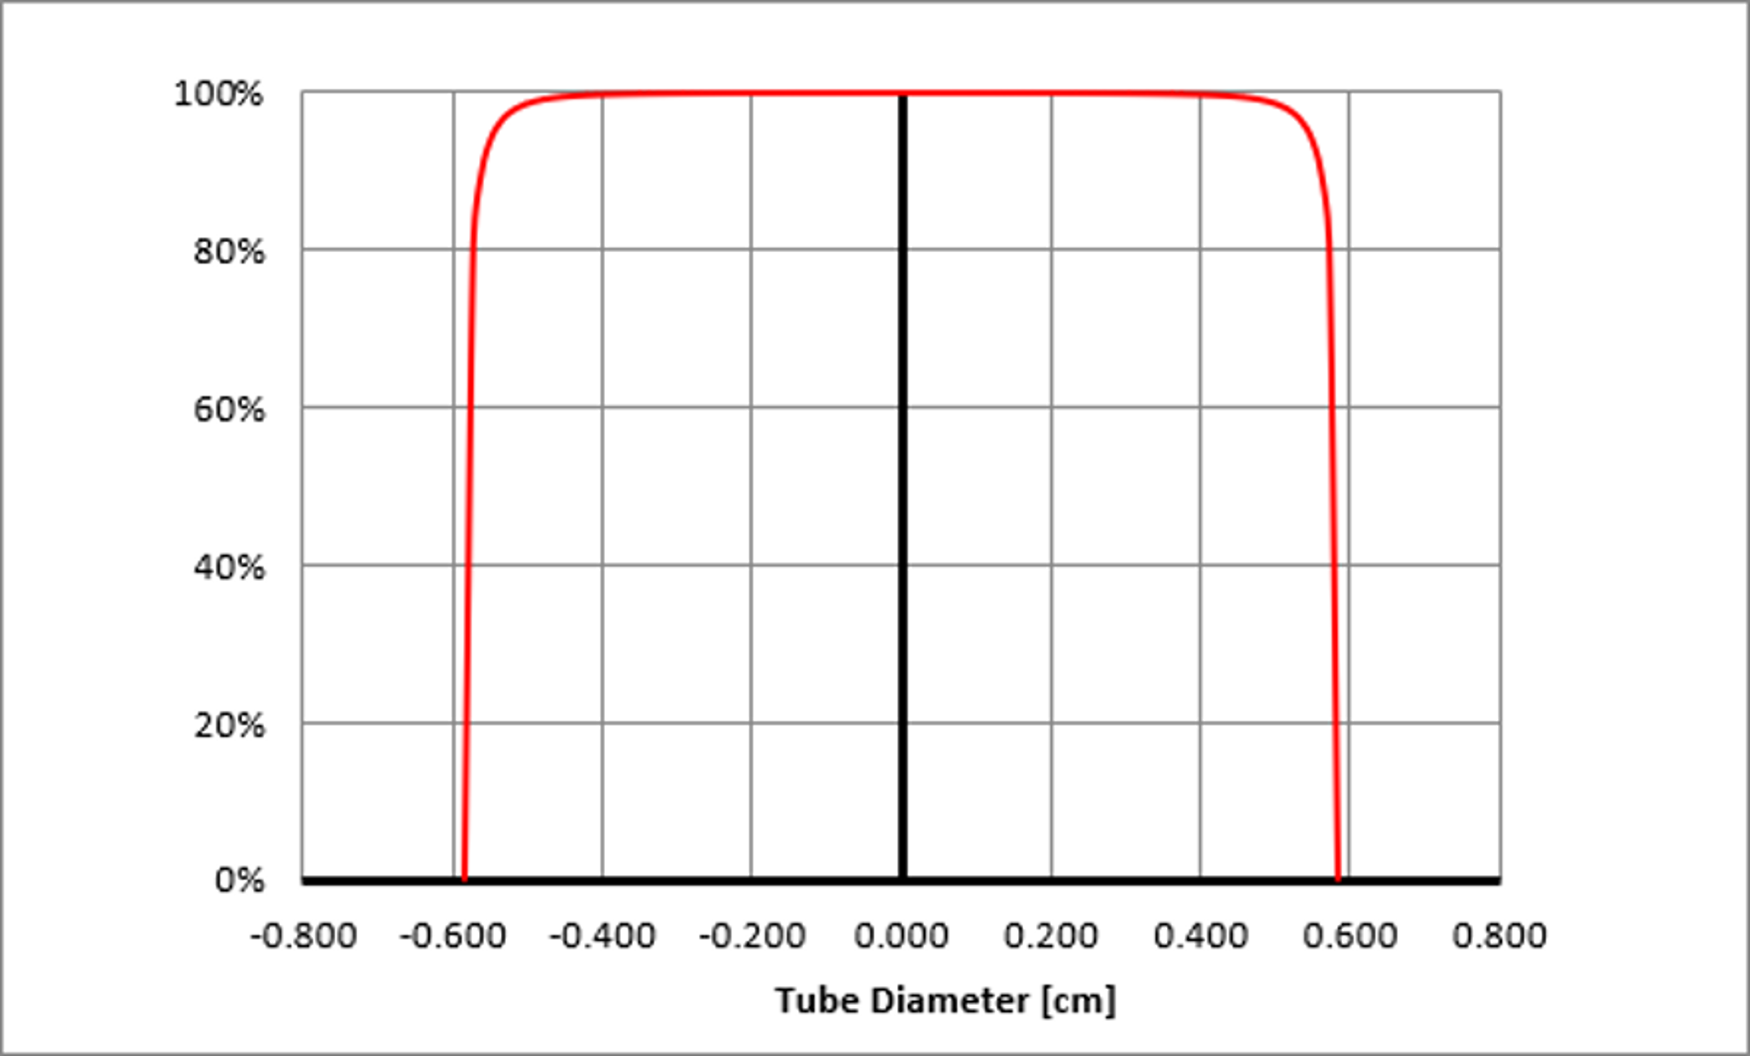
\includegraphics[width=1\linewidth]{figures/chapter4-figs/eff_pos.png}
    \caption{}
    \label{fig:det_eff_diam} 
    \end{subfigure}
    \hfill
    \begin{subfigure}[b]{0.475\textwidth}
    \includegraphics[width=1\linewidth]{figures/chapter4-figs/eff_wave.png}
    \caption{}
    \label{fig:det_eff_wave}
    \end{subfigure}
\caption{Capture efficiency of the LPSD. (a) shows the capture efficiency at 8.9~\AA\ of along the diameter (1.2 cm) of one the LPSD tubes and (b) shows the capture efficiency of 1.2 cm thick LPSD as a function of the incident neutron wavelength.}
\label{fig:det_eff}
\end{figure}
\clearpage}


\subsection{Data Acquisition}

At the SNS, many precisely timed signals are used to operate the accelerator and fill the storage ring and send the proton beam pulse to the target. These time signals are distributed via the Event Link throughout the facility. Other parameters associated with each proton pulse are also available on the Real Time Data Link, (RTDL), which comes from the Ring-To-Beam-Target (RTBT) line proton current monitor. A Beam Diagnostics Card (ETC), receives and decodes timing event triggers from the Event Link and data from the RTDL to produce a timing trigger pulse to synchronize the Data Acquisition System (DAS) hardware with the arrival of the proton pulse at the target. Other key parameters about the proton pulses are read from the RTDL and broadcast to the DAS Timing Cards. These parameters include the accelerator time stamp or Pulse ID, and the proton charge and are used to uniquely identify every neutron pulse.

The critical timing marker to begin the TOF of neutrons is the exact time the proton pulse hits the spallation target. This is called the $T_0$ (Proton on Target or Time Zero) timing reference. This is a timing synchronization signal that is needed to keep the DAS hardware and the neutron beamline components for e.g. ToF choppers synchronized with the 60 Hz neutron pulses for the beamline. The Event Link does not contain an actual event with the exact timing needed to define $T_0$. There is an event called Event 39, or T-Extract, which always occurs at Turn 5050 of the storage ring on the Accelerator timeline each cycle, which has the proper characteristics (phase locked to proton beam, and present each 60 Hz cycle even when beam is not produced or sent to the target1) that is used to create this $T_0$ reference mark. 

Thus, the $T_0$ timing signal is generated as an output from the ETC and becomes the Fiducial Timing Marker or the synchronization pulse to the DAS Timing Hardware. The DAS hardware starts with a delay offset for the purpose of “Framing” each neutron pulse in time, and then measures a local delay from this framing ($T_{sync}$ signal) trigger, until the events are detected in the detectors. This first delay is added by the DAS Timing Card before getting sent to the rest of DAS detector electronics. The $T_{sync}$ pulse then travels by a optical fiber to the top level DAS hardware system, the DSP, and is then distributed down to the lowest detector hardware level where the Local Time Stamp, (LTS), is applied to each neutron as it arrives and is detected. This locally measured delay, LTS, is always a measure of time from the last $T_{sync}$ framing trigger. Thus the $T_{sync}$ delay offset + LTS is a measure of TOF of neutrons in units of 100ns.

The DAQ system for the LPSDs consisted three major components (listed here in order of signal flow) \cite{Beal2021}:
\begin{enumerate}
    \item Two preamplifier boards; one on each end of the LPSDs. The preamplifier board consisted of (in order of signal flow) (i) an output signal protection circuit, (ii) a transimpedance signal amplifier stage to amplify the weak high impedance signal to a large low impedence signal, an inverting voltage amplification stage, and a differential amplifier to drive the low-voltage differential signal (LVDS) to the next step of the signal process \cite{Beal2021, Riedel2012}.
    \item A Read-out-Card (ROC) FPGA that processes and digitizes signals from the preamp. The ROC FPGA is primarily responsible for the event position determination. The LVDS signals from the preamps are passed onto the ROC FPGA and get converted into single ended signals. Next, the ROC FPGA performs three operations on the signal: signal discrimination, signal integration, and position calculation. The analog sum of the two signals from either end of the LPSD is compared against a threshold voltage to determine if the signals represent a neutron event, based on the pulse height. A valid signal then triggers two gated integrators for $1~\mu s$ signal integration. During this integration, two ADC signals are developed to give a proportional measurement of the charge collected from each end of the LPSD for the positional calculation \cite{Beal2021}.
    \item A Digital Signal Processor (DSP) board. The DSP board takes the digitized event positional information from the ROC FPGA, time stamps the events based on the accelerator pulse time/ID and transmits the event information to a computer for data analysis \cite{Beal2021}.
\end{enumerate} 

There are two binary (little-endian format) data files from the DAQ system. The first one is the event mode data file, which consist of ToF in units of 100 ns (32-bit unsigned integer) and positional hits n units of pixels (32-bit unsigned integer) data for the events from each of the 8 LPSD during an acquisition. The second is the pulse ID data file. First part of this file consists of a 64-bit timestamp, broken into two 32-bit integer timestamps in the seconds (first field) and nanoseconds since the EPICS epoch\footnote{Defined as midnight, January 1, 1990.}. All timestamp values are given in UTC time. The next two fields consist of the cumulative event ID (unsigned long long) and the proton charge (double) in units of 10 pC. These binary files were converted to ASCII text files for data analysis.

\section{Analysis and Results}

The event ToF and Positional data was analysed to obtain the transmission of neutrons through the $^3$He analyzer cell. The raw event data contains both the signal and backgrounds, therefore, a scheme to subtract off the background events and determine the signal count rate was developed. This scheme is as follows:

\afterpage{
\begin{figure}
    \centering
    \includegraphics[width=\linewidth]{figures/chapter4-figs/ToF_cut_finder_run408.pdf}
    \caption{Histogram of the raw Time of Flight data for the measurement configuration of $T_0$. The raw data was fitted to extract an approximate $3\sigma$ peak for neutron polarization calculations. The fit residuals are shown underneath.}
    \label{fig:ToFcut}
\end{figure}

\begin{figure}
    \centering
    \includegraphics[width=\linewidth]{figures/chapter4-figs/Pos_cut_finder_run408.pdf}
    \caption{Histogram of the raw positional data for the measurement configuration of $T_0$. The raw data was fitted to extract an approximate $3\sigma$ peak for neutron polarization calculations. The fit residuals are shown underneath.}
    \label{fig:Poscut}
\end{figure}
\clearpage}


\begin{enumerate}
    \item First, the event ToF and positional data was formed into a data structure so that event based cuts could be applied. Only the events which pass any ToF and positional cut will regarded as part of the true signal.
    \item Next, the raw events were histogrammed based on their ToF and positional stamps. The raw ToF histogram for one of the runs is shown in \cref{fig:ToFcut} and the positional hits histogram for the same run is shown in \cref{fig:Poscut}. Qualitatively, the signal peak in the ToF spectrum can be seen at the expected ToF arrival for 8.9~\AA\ as well as at the center of the detector's positional hits data. This means that the statistically significant signal, which corresponds to the neutrons for the different transmission configurations, has to be extracted by subtracting off the background events, which are not part of the primary signal peak, from the entire ToF and positional data. 
    \item A quantitative extraction of signal from the full ToF histogram and detector positional data was performed. To extract signal in the ToF spectrum, the full raw ToF spectrum was fitted using a \texttt{Gaussian+Exponential+Constant} model. From the Gaussian fit on the raw ToF spectrum as shown in \cref{fig:ToFcut}, the mean, $\mu$, and the standard deviation, $\sigma$, were determined. The counts within the $\mu \pm 3\sigma$ range were allocated as the true signal, where the $\pm 3\sigma$ bounds were used to apply the cuts. The events excluded by this range were treated as the background events not overlapping with the signal and were discarded. The full ToF spectrum for all of the runs corresponding to the different transmission measurement configurations was fitted. The largest $3\sigma$ range found from all of the fits on the different configurations was used as to set the ToF cut (3.8 ms to 12.2 ms) for all the transmission measurement configurations.
    \item Similar to the ToF spectrum analysis, a quantitative extraction of signal from the full detector positional data was also performed. The full raw positional data set was fitted using a \texttt{Gaussian+Constant} model. From the Gaussian fit on the positional data as shown in \cref{fig:Poscut}, the mean, $\mu$, and the standard deviation, $\sigma$, were determined. The counts within the $\mu \pm 3\sigma$ range were allocated as the true signal, where the $\pm 3\sigma$ bounds were used to apply the cuts. The events excluded by this positional range were treated as the background events not overlapping with the signal and were discarded. Just like for the ToF Data, the full positional data for all of the runs corresponding to the different transmission measurement configurations were fitted. The largest $3\sigma$ range found from all of the fits was used as the positional cut (pixel400 to pixel550) for all the transmission measurement configurations.

\afterpage{
\begin{figure}
    \centering
    \begin{subfigure}[b]{\textwidth}
    \includegraphics[width=1\linewidth]{figures/chapter4-figs/bkgd_tof.pdf}
    \caption{}
    \label{fig:bkgd_tof} 
    \end{subfigure}
    \begin{subfigure}[b]{\textwidth}
    \includegraphics[width=1\linewidth]{figures/chapter4-figs/bkgd_pos.pdf}
    \caption{}
    \label{fig:bkgd_pos}
    \end{subfigure}
    \caption{Background measurements taken with an active detector but BL13A shutter closed.}
    \label{fig:bkgd}
\end{figure}
\clearpage}
    
    \item Next, the background overlapping with the signal was subtracted off. Because the background in ToF spectrum is not constant due to the presence of thermalized fast neutrons in the early ToF bins, it was determined that the constant background from the positional data should be used to determine the background overlapping with the signal. This is valid since the background taken with the beamline shutter closed showed a constant rate over the entire active area of the detector as shown in \cref{fig:bkgd}. This means that for the range of position pixels excluded by the cuts in step 4, as long as this range is kept at the same as the range cuts used to define the positional signal, the background count rate in that background range will be a good estimator for the background counts rate in the overlapped signal region.
    \begin{equation}
        R = \frac{1}{t_{run}} \int\limits_{left cut}^{right cut} I dx - \frac{1}{t_{run}} \int\limits_{left cut}^{right cut} B dx
    \end{equation}
    where $R$ is the pure signal count rate, $leftcut$ and $rightcut$ are the bounds of the pixel range used, $I$ is the signal with the overlapping background, $B$ is the overlapping background, $dx$ is the pixel bin width and $t_{run}$ is the acquisition time for the associated run. This overlapping background subtraction was performed for all of the runs corresponding to the different transmission measurement configurations.
    \item Lastly, the count rate, $R$, was normalized to the average beam power. The pulse ID data file contains the proton charge deposited for every pulse delivered by the accelerator during the run acquisition time. The average beam power in MW was determined from the total proton charge in an acquisition with the relation:
    \begin{equation}
    \frac{\text{Charge [C]}}{\text{pulse [0.01667 s]}} \times  \frac{1000 \text{[MeV]}}{1 e} \times \frac{1000 \text{[MW $\cdot$ s]}}{1000.0 \text{[MJ]}} 
    \end{equation}

\end{enumerate}

The results of the analysis steps described are shown in \cref{fig:cut} for one of the transmision configurations. This analysis scheme was performed for all of the data runs corresponding to the different transmission measurement configurations illustrated in \cref{fig:pol_scheme} and the results are summarized in \cref{tab:upstreamtrans}. The statistical error on each of the transmission measurements is the counting error\footnote{This is actually the uncertainty on the underlying Poisson distribution for a counting experiment.}, $\sigma = \sqrt{N}$, where N are the raw counts observed in the detector.

\afterpage{
\begin{figure}
    \centering
    \includegraphics[width=\linewidth]{figures/chapter4-figs/Post_cuts_run408.pdf}
    \caption{Analysis steps to identify the ToF and positional signal and backgrounds for the measurement configuration of $T_0$. The first row shows the raw Tof and Positional data. The second row shows the Tof and Positional data after a ToF cut to exclude the background events. The third row shows the ToF and Positional data after a positional cut to further exclude the background event. The fourth row show is the excluded background events in Tof and Positional Space.}
    \label{fig:cut}
\end{figure}
\clearpage}

\afterpage{
\begin{table}
\centering
\caption{Summary of the transmission measurements of 8.9~\AA\ polarized neutron beam through the different configurations of polarized $^3$He cell for the setup shown in \cref{fig:upstream_pol}.}
\label{tab:upstreamtrans}
\begin{tabular}{@{}lccc@{}}
\toprule
State & Beam Polarization State & Analyzer Polarization State & Neutron/s/MW \\ \midrule
$N_0$ & $\uparrow$ & Not Present & 36.8 $\pm$ 0.6 \\
$T_0$ & $\uparrow$ & Unpolarized &  1.85 $\pm$ 0.04 \\
$T$ & $\uparrow$ & $\uparrow$ &  3.57 $\pm$ 0.07 \\ 
$T_{sf}$ & $\downarrow$ & $\uparrow$ & 1.34 $\pm$ 0.03 \\
$T_{sf}^{AFP}$ & $\downarrow$ & $\downarrow$ & 3.25 $\pm$ 0.06 \\
$T^{AFP}$ & $\uparrow$ & $\downarrow$ & 1.21 $\pm$ 0.03 \\ \bottomrule
\end{tabular}
\end{table}
\clearpage}

\afterpage{
\begin{figure}
    \centering
    \begin{subfigure}[b]{\textwidth}
    \includegraphics[width=1\linewidth]{figures/chapter4-figs/trans_det_up.pdf}
    \caption{}
    \label{fig:trans_det_up} 
    \end{subfigure}
    \begin{subfigure}[b]{\textwidth}
    \includegraphics[width=1\linewidth]{figures/chapter4-figs/trans_det_down.pdf}
    \caption{}
    \label{fig:trans_det_down}
    \end{subfigure}
    \caption{Neutron beam intensity measurements at the upstream and downstream locations to determine the transmission loss from the cryomagnet.}
    \label{fig:trans_noapp}
\end{figure}
\clearpage}

\Cref{eq:polarization} can now be used with the transmission measurements results from \cref{tab:upstreamtrans} to determine the neutron beam polarization as:
\begin{equation}
    P_n = 0.83 \pm 0.07_{stat}
\end{equation}
The reported uncertainty is only the statistical uncertainty based on the uncertainty propagation, as described in \cref{app:error}, from each one of the transmission measurements in \cref{tab:upstreamtrans}. 

After the upstream neutron polarimetry was performed, the $^3$He analyzer was moved downstream as shown in \cref{fig:downstream_pol} and repolarized to measure the neutron polarization after the cryogenic magnet. The neutron transmissions with a polarized $^3$He were taken with various cryomagnet magnetic field configurations. They are listed in \cref{tab:down_poldata} of \cref{app:down_poldata}. Despite trying various magnetic field settings, a statistically significant spin contrast was not obtained. Therefore, an accurate neutron polarization downstream of the magnet could not be determined. 

The transmission loss of 8.9~\AA\ neutrons from the cryogenic magnet was also measured based on the setup shown in \cref{fig:trans_setup}. The neutron intensity measured with the detector placed before the magnet is shown in \cref{fig:trans_det_up} and the neutron intensity with the detector placed after the magnet is shown in \cref{fig:trans_det_down}. The intensity measurements are summarized in \cref{tab:trans_noapp}. The fractional transmission was determined to be:
\begin{equation}
    T_n = 0.327 \pm 0.001_{stat}
\end{equation}
The measured intensity upstream in \cref{fig:trans_det_up} shows a Gaussian positional beam profile while the measured intensity downstream in \cref{fig:trans_det_down} shows what looks like overlap of three Gaussian beam profiles. This was attributed to a divergence in the beam intersecting with the cryogenic magnet beam window frames and causing a penumbra of the beam on the detector. This was problematic because the transmission loss is not only coming from the cryomagnet beam windows but the window frames as well. Since the beam is defined by the apertures as shown on \cref{fig:trans_setup}, squeezing the apertures more should reduce the beam divergence and eliminate the problem. The apertures were reduced from 2 cm by 2 cm to 0.5 cm by 0.5 cm and the beam intensities upstream and downstream were measured once again based on \cref{fig:trans_setup}.  The results are shown in \cref{fig:trans_app}. Unfortunately, this data was corrupted, as shown in the pulse height spectrum of \cref{fig:trans_PH_app}, by the presence of amplifier noise as well as modifications of the ADC discriminator settings from a faulty software patch of the DAQ system. By the time these issues were mended, the experimental run plan had to move on to measure the neutron polarization because of the limited SNS beam production left.     



\afterpage{
\begin{table}
\centering
\caption{Integrated and normalized count rates for the neutron beam intensity measurements at the upstream and downstream locations.}
\label{tab:trans_noapp}
\begin{tabular}{@{}lc@{}}
\toprule
State & Neutron/s/MW \\ \midrule
Upstream Intensity &  599.110 $\pm$ 0.003$_{stat}$\\
Downstream Intensity & 195.817 $\pm$ 0.003$_{stat}$ \\ \bottomrule
\end{tabular}
\end{table}
\clearpage}

\afterpage{
\begin{figure}
    \centering
    \begin{subfigure}[b]{\textwidth}
    \includegraphics[width=1\linewidth]{figures/chapter4-figs/trans_det_up_app.pdf}
    \caption{}
    \label{fig:trans_det_up_app} 
    \end{subfigure}
    \begin{subfigure}[b]{\textwidth}
    \includegraphics[width=1\linewidth]{figures/chapter4-figs/trans_det_down_app.pdf}
    \caption{}
    \label{fig:trans_det_down_app}
    \end{subfigure}
    \caption{Neutron beam intensity measurements at the upstream and downstream locations with a smaller aperture to determine the transmission loss from the cryomagnet.}
    \label{fig:trans_app}
\end{figure}
\clearpage}

\afterpage{
\begin{figure}
    \centering
    \begin{subfigure}[b]{\textwidth}
    \includegraphics[width=1\linewidth]{figures/chapter4-figs/trans_det_up_PH_app.pdf}
    \caption{}
    \label{fig:trans_det_up_app} 
    \end{subfigure}
    \begin{subfigure}[b]{\textwidth}
    \includegraphics[width=1\linewidth]{figures/chapter4-figs/trans_det_down_PH_app.pdf}
    \caption{}
    \label{fig:trans_det_down_app}
    \end{subfigure}
    \caption{Pulse height spectrum of the transmission beam intensity data taken with a smaller aperture.}
    \label{fig:trans_PH_app}
\end{figure}
\clearpage}

\subsubsection{Proton Charge}

\afterpage{
\begin{figure}
    \centering
    \begin{subfigure}[b]{\textwidth}
    \includegraphics[width=\textwidth]{figures/chapter4-figs/Full_PCharge_run416.pdf}
    \caption{}
    \label{fig:fullPcharge} 
    \end{subfigure}
    \begin{subfigure}[b]{\textwidth}
    \includegraphics[width=\textwidth]{figures/chapter4-figs/Part_PCharge_run416.pdf}
    \caption{}
    \label{fig:partPcharge}
    \end{subfigure}
    \caption{Proton charge for the $T_0$ run. (a) shows the total proton charge for each pulse accumulated for the run and (b) shows the proton charge accumulated during a stable beam period.}
    \label{fig:Pcharge}
\end{figure}
\clearpage}

As stated earlier, the proton charge accumulated over the entire acquisition time for a run was used to normalize the count rate to account for proton beam variations in the incident neutron flux. At the SNS, the measured proton charge set to ADC is quantized as a 16-bit integer representation of charge per pulse scaled to provide the desired units. At low charge-per-pulse, the SNS does change the range on the digitizer to avoid any quantization errors \cite{Blokland2023}. However at full power, the proton charge is calibrated to be within 2\% of the true value with 0.5\% reproducibility \cite{Blokland2023}. Furthermore, from the data collection of neutron beam with no analyzer in place as shown in \cref{fig:Pcharge}, the resolution in the proton charge can be noted as a little less than $0.002\times10^5$, or $6.8\times10^{-4}$ relative to the average charge value. Therefore, the full output precision of the proton charge was not used. This run had about $1.3\times10^5$ pulses, which included some proton beam-down/ramping time, as shown in \cref{fig:beampower}. These bad pulses are shown in \cref{fig:fullPcharge}, where some proton charge deviated from the nominal proton charge at full beam power due to accelerator instability. For all the data runs collected, these ``bad" pulses turned out to be only about 0.2\% of the of total charge per pulse collected. The variance of the nominal proton charge peak in \cref{fig:partPcharge} is, in principle, the sum in quadrature of the quantization error, the uncertainty in the proton charge measurement, and the dispersion in the true proton charge value (assuming all of them are independent of each other). Since the variance in the proton charge accumulated is shown to be small and additionally, only the data at the nominal proton charge was considered, the variance from the proton charge normalization was be neglected for the neutron polarization and transmission measurements.

\afterpage{
\begin{figure}
    \centering
    \includegraphics[width=\textwidth]{figures/chapter4-figs/BeamPower416.pdf}
    \caption{Beam power for the $T_0$ run. The nominal beam power of the SNS during the summer 2023 neutron production was 1.6 MW. There are drops in the power as seen in figure due to accelerator instability.}
    \label{fig:beampower}
\end{figure}
\clearpage}

\subsection{Systematic Effects}

Since the underlying quantities being measured to determine the neutron beam polarization are the transmission measurements through various configurations, any changes in neutron transmission from sources other than the intended configuration setup can lead to a systematic shift in the actual transmission and subsequently, cause a systematic uncertainty in the neutron beam polarization extraction. This sections describes the possible effects which can give rise to a systematic uncertainty in the neutron beam polarization.

\subsubsection{Non-Poisson Variations of the Neutron Beam}

The uncertainty on the neutron polarization can be limited by the non-Poisson variations of the neutron beam produced by the SNS at nominal power. Previous neutron polarimetry experiment at FnPB beamline 13 has shown that the measurement is not limited by the non-Poisson variation in the neutron flux because it is far smaller than the neutron transmission variation from the different configuration of the polarized $^3$He cell \cite{Musgrave2018}. In that experiment, non-Poisson uncertainty on the neutron polarization was measured by performing neutron polarimetry at several locations along the neutron flight path \cite{Musgrave2018}. The systematic uncertainty in the neutron polarization from non-Poisson fluctuations beam was determined to be $2 \times 10^{-3}$, including the statistical uncertainty \cite{Musgrave2018}. 

During the Summer 2023 data taking campaign, the direct neutron beam flux on the LPSD detector was measured for 5 mins, in succession, to check for non-Poisson variations of the neutron beam. The variation is shown in \cref{fig:beam_fluc}. The integral up to the $\pm 1\sigma$ of the Gaussian fit to the counts during a single acquisition is within the $1\sigma$ error bar of the assumption of constant proton power normalization consistently used in the analysis. Therefore, the non-Poisson noise in the neutron beam can be assumed as stable and the normalization assumption is good at the sub\% level. In hindsight, this check for beam variation should have been done more frequently over the span of the Summer 2023 SNS neutron production cycle.  

\afterpage{
\begin{figure}
    \centering
    \includegraphics[width=\textwidth]{figures/chapter4-figs/beamstability.png}
    \caption{Variation in neutron count rate over the course of 30 mins. Each run represents 5 mins of acquisition time.}
    \label{fig:beam_fluc}
\end{figure}

\clearpage}


\subsubsection{$^3$He Cell Polarization Fluctuations}

\afterpage{
\begin{figure}
    \centering
    \includegraphics[width=\textwidth]{figures/chapter4-figs/Spinup_graph_jun26.png}
    \caption{Build up of the in situ $^3$He polarization over the course of the measurement period. The red points are the measured value and the green curve is the increasing form exponential decay fit.}
    \label{fig:live_spinup}
\end{figure}
\clearpage}  

The advantage of the neutron polarimetry technique described in \cref{sec:PT} is that the neutron polarization can be determined by relative neutron transmission measurements through a polarized $^3$He cell without knowing the $^3$He polarization. This is valid however, if the $^3$He cell polarization is stable over the course of the measurement. Any variations in $^3$He polarization of the cell will hamper its ability to analyze the spin contrast of the neutron beam. For the neutron polarimetry performed, this effect is remedied by the fact that during the polarization measurements, the $^3$He cell polarization is maintained by a live in situ SEOP system as described in \cref{ch:polHe}. The cell was also kept in a continuous holding magnetic field with minimal gradients using a magnetostatic cavity as described in \cref{ch:polHe}. This live maintenance of the $^3$He polarization can be seen in \cref{fig:live_spinup}. Nevertheless, performing AFP and FID NMR can lead to depolarization of $^3$He.  

The $T_1$ time of the $^3$He cell used in the experiment, Soccer, was measured to be $45 \pm 2$ hours as shown in \cref{fig:spindown}. This time was measured by taking FID NMR measurements of polaried $^3$He every 3 hours with the SEOP system powered off. A small $^3$He polarization loss of  $0.63\% \pm 0.12\%$ from the FID NMR exists as shown in \cref{fig:NMRLoss}. After correcting for the FID NMR loss, the true $T_1$ time was found to be $56 \pm 2.5$ hours. This indicates that the short 3 hour FID NMR time interval can vary the much longer $T_1$ relaxation time.  Again this NMR $^3$He depolarization effect was negated since, $^3$He cell was undergoing constant optical pumping. Nevertheless, a worst case upper limit on the neutron polarization can be established by assuming the in situ system was shut off and using the uncorrected $T_1$ time of 45 hours to account for any variation in $^3$He polarization.

The run time for transmission measurements of different configurations of \cref{fig:pol_scheme} was around 30 minutes. A $T_1$ time of 45 hours will cause the polarize $^3$He to depolarize by a factor of $9.9 \times 10^{-3}$ during the 30 minute time interval. Similarly for AFP NMR, a loss of 0.053\% per flip of 350 ms duration was observed, which leads to a $^3$He polarization loss of $6 \times 10^{-5}$. Using \cref{eq:t} and \cref{eq:tsf}, the effect of the $T_1$ relaxation time on the neutron transmission through analyzer cell was be taken into account as:
\begin{equation}
    T = N_0e^{-\zeta}\cosh{\left(\zeta e^{-\frac{t}{T_1}}P_{He}\right)}\left(1+P_n\tanh{\left(\zeta e^{-\frac{t}{T_1}}P_{He}\right)}\right)
\end{equation}
and
\begin{equation}
    T_{sf} = N_0e^{-\zeta}\cosh{\left(\zeta e^{-\frac{t}{T_1}}P_{He}\right)}\left(1+\left(1-2\epsilon_{sf}\right)P_n\tanh{\left(\zeta e^{-\frac{t}{T_1}}P_{He}\right)}\right)
\end{equation}
where $\zeta= nl\frac{\sigma_0}{\lambda_0}\lambda(t)$. Then, \cref{eq:polarization} was used to calculate the neutron polarization. The effect of the $T_1$ relaxation time of the polarized $^3$He cell was an adjustment of less than $1.1 \times 10^{-2}$ to the neutron beam polarization. This effect, again assuming failure of the in situ SEOP system, is much less than the statistical uncertainty of the measured beam polarization.

%The width of the pseudo-Gaussian of about 0.7\% (assuming you properly throw away anything "not full power" by some perfect but unspecified cutting algorithm) will give the dispersion in the reported value, which would be the sum in quadrature of the discretization error, the uncertainty in the actual measurement, and the dispersion in the true value (assuming those are independent, which is pretty likely if you limit your examination to nominally full charge pulses).

%In all fairness, the way to propagate those errors properly / rigorously will depend strongly on what you're actually doing. If you want to know something that really does boil down to neutrons per proton, you will have to deal with a rigorous analysis of the beam charge value. If you really want neutrons / neutron (e.g., neutrons with spin up per any neutron) then you can get there via a neutron beam monitor assessment (neutrons in M3 per neutron in M1) OR via the chain involving neutrons / proton per neutrons / proton - all the same neutron based uncertainty plus twice the proton beam monitor uncertainty. No judgment from me on which is better, you just want to correctly treat whichever you're actually using. Doing so SOME ways might involve either throwing away data from runs that vary by something you can't assess or by measuring some system non-linearities that aren't well evaluated, but again that's just an assessment, not a judgment.

%Method 1: count neutrons per proton in M3 with no analyzer (N); count neutrons per proton in M3 with analyzer (Nup), throw out all pulses that aren't within X\% of nominal full pulses, happen within Y days of the moderator being filled, etc. Contributing uncertainties include two counting uncertainties, double the proton charge measurement uncertainty.

%Method 2: count neutrons per proton in M3 with no analyzer; count neutrons per proton in M3 with analyzer, taking ALL the pulses. Contributing uncertainties include two counting uncertainties, double the proton charge measurement uncertainty, any nonlinearity uncertainties arising from moderator performance w.r.t. proton beam power (note that this nonlinearity varies with wavelength), variable dead time effects within the beam monitor (or saturation / nonlinearity if it's not a counting detector), variations in spectral distribution with hydrogen age, temperature, etc. This will by definition be a larger uncertainty than in Method 1 for equivalent counts, but may be easier to get to higher counts in the same time because you don't have the same constraints on consistent performance.

%Method 3: count neutrons in M3 per neutron in M1 with and without analyzer, taking all pulses. Four counting uncertainties, dead time corrections, PLUS the new one - systematic errors in binning the two time spectra (at different distances) into the same wavelength histogram (or fitting, or however you choose to turn the time spectrum into a wavelength spectrum).

%Method 4: Like 3 but cutting out some pulses. Four counting uncertainties and the time-to-wavelength systematics. The dead time effects cancel.


\subsubsection{Moderator Fluctuations}

\afterpage{
\begin{figure}
    \centering
    \includegraphics[width=\textwidth]{figures/chapter4-figs/mod_temp.pdf}
    \caption{Temperature in Kelvins of the hydrogen moderator over the course of the summer 2023 neutron production.}
    \label{fig:mod_temp}
\end{figure}
\clearpage}

There are non-linear contributions to the neutron flux from fluctuations in the performance of the hydrogen moderator caused by hydrogen age as well as density and temperature variations \cite{Carpenter1977}. The non-linear behavior can run about 10\% per MW - for e.g. the number of 5~\AA\ neutrons per MW*sec measured at 1.7 MW and 60 Hz is approximately 85\% of  the true value if scaled from the the number of 5~\AA\ neutrons per MW$\cdot$s measured at 11 kW and 60 Hz. The hydrogen moderator is equipped with cryogenic circulator and heat exchanger to maintain the temperature and density distribution. \Cref{fig:mod_temp} shows the temperature variations in the hydrogen moderator over the course of the summer 2023 SNS neutron production was stable. 

It is also known that the hydrogen moderator performance depends on the ortho-hydrogen and para-hydrogen ratio \cite{Squires1955, Ooi2011}. The scattering cross-section of para-hydrogen for 1 meV neutrons under is about a factor of 500 smaller than that of ortho hydrogen \cite{Grammer2015}. At about 20 K operating temperature of the moderators, the thermodynamic equilibrium hydrogen composition is 99\% para hydrogen, meaning over the course of the filling of the moderator, the para-hydrogen concentration gradually increases \cite{Ooi2011, Kai2005}. \cite{Ooi2006} have measured a gradual change of the neutronic performance of the hydrogen moderator. Currently, the SNS does not have an experimental scheme to measure the ortho-para concentration ratio in the hydrogen moderators. However, the time constant of ortho-to-para conversion is very long; about 48,000 hours for a conversion from 25\% para to 99\% para hydrogen \cite{Ooi2011}. This time scale is much larger then the time scale over which the polarization and transmission measurements were conducted. Therefore, the fluctuations in neutron transmission due to moderator performance variations were neglected.

\subsubsection{Humidity Fluctuations}

Because the polarimetry components were placed in an open air environment, any change in humidity can vary the measured neutron transmission. \cite{Zhang2023} show that commercial HVAC system usually maintain the room humidity to around 50\%-60\%. At these humidity levels, the density of air, $1.11\times10^{-3}$~g cm$^{-3}$, does not fluctuate significantly enough to cause a major change in neutron transmission. There is a 4\% loss in 8.9~\AA\ neutron transmission for every meter of 50\%-60\% humid air at normal temperature and pressure. Since the density of air likely did not change in between the measurements, this loss was present for all the transmission measurements and got cancelled out in the analysis. 

\subsubsection{Detector Efficiency Variations}

Any variations in the efficiency of the LPSD detectors over the course of the measurement period can also lead to systematic uncertainties in the neutron polarization measurements. Over the lifetime of the SNS, the SNS detector scientists have not observed any degradation in performance of $^3$He LPSDs unless in the event of catastrophic damage \cite{Berry2023}. The chances $^3$He gas leakage are low to none, since the pulse height spectrum would indicate a variation in the signal charge collected. Any odds of depletion of $^3$He in the LPSDs are also very low since for nominal neutron count rates of $1\times10^4$ neutron s$^{-1}$ cm$^{-2}$, only about 1ppm of $^3$He atoms would get depleted in 1000 years. 

%\subsection{Corrections to the Transmission Measurement}

%As shown in \cref{fig:trans_noapp}, the beam profile measured downstream of the cryomagnet was too broad. So much so that that the broad neutron beam was interfering with the cryomagnet beam window frames causing a neutron beam penumbra on the detector. This is evident based the reduced intensity neutron signals on the flanks of the primary signal shown in \cref{fig:trans_noapp}. The obvious solution to this problem was to measure the transmission with a tighter beam collimation. However, as explained in the previous section, issues with the neutron detector prevented from doing so.  

%A virtual collimation can be applied on the original beam profile to isolate only the neutrons transmitting through the neutron beam windows of the cryomagnet. These neutrons could then be back tracked to their corresponding signal in the upstream detector. The ratio of the resulting collimated events should give a more accurate depiction of the transmission loss of the neutron beam through the cryomagnet. 

%To do this, the transmission setup, as shown in \cref{fig:trans_setup} but without the cryomagent, was constructed in the McStas neutron ray tracing program. The complete 8pack detector geometry was built to account for the geometric and neutron capture efficiencies of the detector. An event mode detection was used to reconstruct the    


%so did a Mcstas sim without the cryomagnet and see if virtual collimation can be used to collimate the penumbra and measure an accurate beam profile and transmission.

\section{Beam Window Transmission Measurements using SANS}

\subsection{General Purpose SANS Beamline at HFIR}

In Small Angle Neutron Scattering (SANS), elastic neutron scattering, arising from spatial changes, typically of length order of nm, in the nuclear scattering length densities (SLD) of a material, is used to characterize the sub-structure of materials \cite{Pynn1990, Hammouda2008, Feigin2013, Glinka2004}. In material science, SANS along with small angle X-ray scattering (SAXS) are used in a complimentary manner to understand the complex structure of materials. Purpose-built SANS instruments produce intense neutron beams with cross-sectional area up to several cm$^2$, allowing for deeper penetration of neutrons, which is useful for studying bulk samples on the order of millimeters \cite{Feigin2013}. For the purposes of nEDM experiment, SANS technique is ideal for characterizing the transmission loss and coherent scattering of cold neutrons from the beam window materials. The CG2 GP-SANS machine at HFIR is suitable for this proposed research because it can provide 8.9~\AA\ neutrons with a $\Delta \lambda$/$\lambda$ of 0.13, a high-count rate for good statistics in a short time \cite{Wignall2012, Heller2018}. The instrument is equipped with large scattering acceptance detector arrays, which can provide a scale of the SANS induced beam divergence for the beam window materials \cite{Wignall2012, Heller2018}.

\afterpage{
\begin{figure}
    \centering
    \includegraphics[width=\linewidth]{figures/chapter4-figs/SANS_pic.png}
    \caption[A schematic illustration of a SANS instrument.]{A schematic illustration of a SANS instrument. Figure taken from \cite{Glinka2004}.}
    \label{fig:SANS_pic}
\end{figure}
\clearpage}
    
A schematic of a typical SANS experimental setup is shown in \cref{fig:SANS_pic}. A neutron beam is incident on a sample and the transmitted and scattered neutrons are detected by a position sensitive two dimensional detector. SANS measures the scattered neutron intensity, $I(Q)$, as a function of the scattering vector, $Q$, which in the case of GP-SANS is defined as:
\begin{equation}
    Q = \frac{4 \pi}{\lambda}\sin{2 \theta}
    \label{eq:Q}
\end{equation}
where, $\theta$, is the scattering angle and $\lambda$ is the incident neutron wavelength \cite{Pynn1990, Hammouda2008, Feigin2013, Glinka2004}. The length scale probed is approximately proportional to $\lambda$/$\theta$ under the small angle approximation, and is generally in the range of 1 to a few hundred nm. The resolution on Q can be approximated as $ \Delta Q$/$Q$ $\propto$ $\Delta \lambda$/$\lambda$ + $\Delta\theta$/$\theta$. Since $\Delta \lambda$/$\lambda$ is restricted by the instrument's velocity selector, the dominant contribution to the resolution is from $\Delta\theta$/$\theta$, which in the small angle limit is can be approximated as $a/L$, where $a$ is the sample aperture size and $L$ is the distance from the sample to the detector \cite{Pynn1990, Hammouda2008, Feigin2013, Glinka2004}. If the sample aperture is fixed, then the scale of Q (i.e. $\theta$ ) is varied by moving the detector away from or close to the sample. hence, large Q is used to probe small length scale features with the detector close to sample and small Q is used to probe larger objects by moving the detector far away from the sample.

\subsection{SANS Studies of Beam Windows}

The purpose of this test was to measure the transmission and scattering loss of 8.9Å neutrons from samples of thin metal window materials at ambient temperature. Two samples of the material candidates for the thin metal windows, Magnesium/Aluminum alloy (AZ31B), Zircaloy-4 (Zr-4), and two samples of the MFM layers of the nEDM cryomagnet, the lead and Metglas, were tested. The properties of these materials are listed in \cref{tab:SANS_mat}. These materials were chosen because of their high transparency to neutrons, suitable mechanical properties as cryogenic vacuum windows and minimal neutron activation. It was important to characterize (i) the transmission, to ensure the window material is not compromising the 8.9~\AA\ flux and (ii), the scattering, to ensure the material will not broadening the beam divergence, which may interact with the off-beam axis components of the main nEDM@SNS experiment; producing large backgrounds. To illustrate this further, the nEDM@SNS experiment's neutronics geometry has to be considered. There is a 1.5 m gap between the thin metal vacuum window at end of the neutron guide and the measurement cell entrance. Each measurement cell is 7.5 cm wide. Therefore, the critical angle of beam acceptance of the measurement cells comes out to be 1.43\degree. The objective of these studies was characterize the sub-structure dependent neutron scattering for the different samples.

\subsubsection{Analysis and Results}

NIST neutron cross section library was used to obtain a first order estimate of 8.9~\AA\ neutron transmission and scattering from the materials in question \cite{Sears1992}. As shown in \cref{tab:SANStable}, the $1/e$ attenuation of the materials is much larger than the required thickness and the scattering cross section is small, therefore, for 8.9~\AA\ neutrons, minimal transmission and scattering loss is expected.

\afterpage{
\begin{table}
\centering
\caption{Properties of the beam window materials.}
\label{tab:SANS_mat}
\begin{tabular}{@{}llcc@{}}
\toprule
Sample & Mass Percent Composition & Density {[}g cm$^{-3}${]} & Thickness {[}cm{]} \\ \midrule
Mg AZ31B & Mg-96\%, Al-3\%, Zn-1\% & 1.77 & 0.274 \\
Zircaloy-4 & Zr-98\%, Sn-1.5\%, Fe-0.2\%, Cr-0.1\% & 6.56 & 0.238 \\
Lead & Pb-100\% & 11.34 & 0.08 \\
Metglas-2826MB3 & Fe-45\%, Ni-45\%, Mo-7\%, B-3\% & 7.90 & 0.0029 \\ \bottomrule
\end{tabular}
\end{table}
\clearpage}

\afterpage{
\begin{table}
\centering
\caption[Calculated neutron scattering cross section (coherent and incoherent) and attenuation length (absorption) from NIST Neutron Cross Section Library for the proposed materials.]{Calculated 8.9~\AA\ neutron scattering cross section (coherent and incoherent) and attenuation length (absorption) from NIST Neutron Cross Section Library for the proposed beam window materials \cite{Sears1992}.}
\label{tab:SANStable}
\begin{tabular}{@{}lccc@{}}
\toprule
\multirow{2}{*}{Sample} & \multicolumn{2}{c}{Scattering Cross Section {[}cm$^{-1}${]}} & \multirow{2}{*}{Attenuation Length {[}cm{]}} \\ \ctoprule(lr){2-3}
 & Coherent & Incoherent &  \\ \midrule
Mg AZ31B & 0.155 & 0.004 & 65.02 \\
Zircaloy-4 & 0.278 & 0.001 & 23.02 \\
Lead & 0.366 & 0 & 35.84 \\
Metglas-2826MB3 & 0.949 & 0.260 & 0.019 \\ \bottomrule
\end{tabular}
\end{table}

\clearpage}

The GP-SANS instrument was configured for the measurement described here in the following way. The velocity selector was tuned to provide 8.9~\AA\ neutrons with a $\Delta \lambda$/$\lambda$ of 0.13. The sample aperture was 2 mm. Since the primary motivation for test was to study the incoherent scatter ring from the samples, the Q was set to low (L = 1 m) and high (L = 8 m). 


%Attenuators and apertures will be used to reduce the initial beam count rate, so as not to saturate the detectors and obtain an accurate transmission and scattering loss from the initial flux. Firstly, beam intensity and spot size will be measured with the detector upstream of the sample mount to characterize the initial flux. The samples will then be loaded, one at a time, and the detector will then be placed on the downstream end. The beam intensity and scattered beam spot size will be measured for each sample.

To understand the sources of scattering, the differential cross section $\frac{d\Sigma(Q)}{d\Omega}$ , is the primary quantity extracted from a SANS measurements \cite{Pynn1990, Hammouda2008, Feigin2013, Glinka2004}. It can be interpreted as the number of neutrons per second [neutrons sec$^{-1}$] scattered onto a solid angle unit by the incident neutron flux [neutrons  sec$^{-1}$ cm$^{-2}$] and upon normalizing by the sample volume unit, has the dimensions of cm$^{-1}$. Integrating this over the solid angle gives the total absolute cross section, $\Sigma_{total} = \Sigma_{absorption} + \Sigma_{incoherent} + \Sigma_{coherent}$, where $\Sigma_{coherent}$ is from coherent scattering, which comes from the structural information of sample, $\Sigma_{incoherent}$ comes from the flat isotropic scattering background and $\Sigma_{absorption}$ is the neutron absorption. From this, the measured count rate can be used to determine the the differential cross section as:
\begin{equation}
    \frac{d\Sigma(Q)}{d\Omega} = \frac{1}{ I_0 \cdot A \cdot d \cdot \Delta \Omega \cdot \epsilon \cdot t} I(Q)
\end{equation}
where $I_0$ is the incident neutron flux on a sample of area, $A$, and thickness, $d$, scattered on the solid angle, $\Delta \Omega$, of each pixel of the detector with efficiency, $\epsilon$, for a counting time, $t$. For these measurement, the thickness of the samples is based on the engineering design requirements of the nEDM cryomagnet beam windows. This means that multiple neutron scattering within the sample can also be an issue. For this test, the sub-structure dependent neutron scattering was of primary interest.

To analyze the data, all the contributing factors to the detector signal need to be measured. The first factor is the actual SANS scattering from sample. The second factor is the scattering from sources other than sample. These sources include scattering from empty sample holder, scattering from collimation slits and scattering from air. This determined by beam measurement with no sample in place, with lithium apertures installed and placing the detector assembly in a vacuum chamber. The third factor is ambient backgrounds and electronic noise. These sources are the detector dark current, ambient neutrons in the reactor cold guide hall building and Cosmic radiation. The background measurement comes from a blocked beam measurement using Cadmium sheet. An isotropic scattering attenuator (PMMA acrylic in this case) is used to characterize the detector sensitivity due to variations in detector tubes/pixels. PMMA acrylic is also used as an attenuator reduce the direct beam flux to prevent detector high count rate dead time inefficiencies. 

The raw intensity measured from SANS is:
\begin{equation}
\begin{aligned}
        I_{sample} = & \left( I_0 \cdot A \cdot d \cdot \Delta \Omega \cdot \epsilon \cdot t \right) T_{sample+nosample} \\ & \times \left( \left(\frac{d\Sigma(Q)}{d\Omega}\right)_{sample}  + \left(\frac{d\Sigma(Q)}{d\Omega}\right)_{nosample} \right) + I_{blockedbeam} 
\end{aligned}
\end{equation}
then, the raw intensity with no sample in place is measured as:
\begin{equation}
    I_{nosample} = \left( I_0 \cdot A \cdot d \cdot \Delta \Omega \cdot \epsilon \cdot t \right) T_{nosample} \left( \left(\frac{d\Sigma(Q)}{d\Omega}\right)_{nosample}      \right) + I_{blockedbeam} 
\end{equation}
where the background intensity is measured as:
\begin{equation}
    I_{BKGD} =  I_{blockedbeam} 
\end{equation}
The raw sample intensity is corrected after subtracting the backgrounds and no sample intensity. Data is also normalized to the total count rate to account for the counting time and the Poisson noise in the beam intensity from the reactor during the measurements. 
\begin{equation}
    I_{corrected} = \left( I_{sample} - I_{BKGD} \right) - \left(  \frac{T_{sample}}{T_{no sample}} \right) \left( I_{nosample} - I_{BKGD} \right)
\end{equation}
The data is further calibrated based on the normalized detector sensitivity taken with a known PMMA acrylic sample at the start of each reactor cycle:
\begin{equation}
    I_{calibrated} =  \left(  \frac{I_{corrrected}}{I_{detector sensitvity}} \right) 
\end{equation}
where
\begin{equation}
    I(Q)_{cal} = \left( I_0 \cdot A \cdot d \cdot \Delta \Omega \cdot \epsilon \cdot t \right) T_{sample} \left( \frac{d\Sigma(Q)}{d\Omega}  \right)_{sample} 
\end{equation}
This reduced data is then scaled to absolute units by the direct beam flux method, where a direct beam with an attenuator is measured as $ I_{direct} = I_0 \cdot A \cdot d \cdot \Delta \Omega \cdot \epsilon \cdot t $. Therefore the final differential cross section intensity in units of [$cm^{-1}$] becomes:
\begin{equation}
   \left( \frac{d\Sigma(Q)}{d\Omega}  \right)_{sample} = \left ( \frac{I(Q)_{cal}}{I_{direct}}  \right)  \left ( \frac{T_{attenuator}}{T_{sample+nosample}}  \right) \frac{1}{d} 
\end{equation}

%Standard Sample Calibration
%- Use a sample with known absolute scattering cross-section at Q=0.
%- Measure the standard sample with the exactly same configuration
%\begin{equation}
 %   I(Q=0)_{Standard} = \left( I_0 \cdot A \cdot d \cdot \Delta \Omega \cdot \epsilon \cdot t \right) T_{standard} \left( \frac{d\Sigma(Q)}{d\Omega}  \right)_{standard}
%\end{equation}
%\begin{equation}
   %\left( \frac{d\Sigma(Q)}{d\Omega}  \right)_{sample} = \left ( \frac{I(Q)_{cal}}{I(Q=0)_{standard}}  \right)  \left ( \frac{T_{standard}}{T_{sample}}  \right) \left (\frac{d_{standard}}{d_{sample}} \right) \left( \frac{d\Sigma(Q=0)}{d\Omega}  \right)_{standard}
%\end{equation}

\afterpage{
\begin{figure}
    \centering
    \begin{subfigure}{0.40\linewidth}
        \includegraphics[width=\linewidth]{figures/chapter4-figs/Zr-lowQ.pdf}
 
    \end{subfigure}
    \hfil
    \begin{subfigure}{0.40\linewidth}
        \includegraphics[width=\linewidth]{figures/chapter4-figs/Zr-highQ.pdf}
   
    \end{subfigure}

    \begin{subfigure}{0.40\linewidth}
        \includegraphics[width=\linewidth]{figures/chapter4-figs/AZ31-lowQ.pdf}
   
    \end{subfigure}
    \hfil
    \begin{subfigure}{0.40\linewidth}
        \includegraphics[width=\linewidth]{figures/chapter4-figs/AZ31-highQ.pdf}
  
    \end{subfigure}

    \begin{subfigure}{0.40\linewidth}
        \includegraphics[width=\linewidth]{figures/chapter4-figs/Pb-lowQ.pdf}
   
    \end{subfigure}
    \hfil
    \begin{subfigure}{0.40\linewidth}
        \includegraphics[width=\linewidth]{figures/chapter4-figs/Pb-highQ.pdf}
 
    \end{subfigure}

        \begin{subfigure}{0.40\linewidth}
        \includegraphics[width=\linewidth]{figures/chapter4-figs/Metglas-lowQ.pdf}

    \end{subfigure}
    \hfil
    \begin{subfigure}{0.40\linewidth}
        \includegraphics[width=\linewidth]{figures/chapter4-figs/Metglas-highQ.pdf}

    \end{subfigure}

\caption{2D histograms of the SANS scattering from the beam window samples tested.}
\label{fig:SANS_2D}
\end{figure}
\clearpage}

\afterpage{
\begin{figure}
    \centering
    \begin{subfigure}[b]{\textwidth}
    \includegraphics[width=1\linewidth]{figures/chapter4-figs/Combined_SANS.pdf}
    \caption{}
    \label{fig:sansvq} 
    \end{subfigure}
    \begin{subfigure}[b]{\textwidth}
    \includegraphics[width=1\linewidth]{figures/chapter4-figs/Combined_SANSvstheta.pdf}
    \caption{}
    \label{fig:sansvtheta}
    \end{subfigure}
    \caption{SANS intensity as a function of the scattering vector, $Q$, (a) and scattering angle, $\theta$, (b) for the beam window material samples.}
    \label{fig:SANSvqvtheta}
\end{figure}
\clearpage}

The two dimensional scattering phase space intensity distribution for the four beam window materials taken at high Q and mid Q are shown in \cref{fig:SANS_2D}. The unscattered beam is masked off to emphasize the scattered beam. The intensity distribution can be averaged over the entire annular scattering phase space to obtain a one dimensional SANS plot shown in \cref{fig:sansvq}. \Cref{fig:sansvtheta} is plotted as a function of scattering angle, $\theta$, by using \cref{eq:Q}. This is done for ease of interpretation of data in terms of the neutron beam divergence. \Cref{fig:sansvtheta} shows that neutron beam divergence from the SANS is much smaller than the neutron beam acceptance angle of the nEDM@SNS experiment's measurement cells. The figure also shows that the isotropic incoherent scattering is minimal for all the samples except for Metglas. There is some uncertainty on the Metglas sample because the data was taken for not long enough statistics. The scattered beam intensity shows the expected power law curve for all the samples except for AZ31B, which indicates a possible sub-structure in the AZ31 sample. The AZ31B sample was found to have a shear strain running through the middle, which could have caused this SANS feature. 

\subsubsection{Sample Transmission}

The measured transmission of the sample, $T_{sample}$, is defined as the ratio of transmission through the sample to the transmission without sample, $T_{nosample}$. Both transmissions measurements were taken with the PMMA attenuator in place (attenuation factor of $\times2000$) to prevent the detector from saturating. For the analysis, the transmission measurements were taken with the detector located at the mid Q range (8 m from sample) to find the region of interest for the zero angle neutrons cut. Based on the SANS instrument settings, the beam size was estimated to be 51.1 mm at the mid Q range \cite{Debeer-Schmitt2023}. Then, the actual transmission data was taken at high Q range (1 m from sample) with the beam size was estimated to be 9.9 mm \cite{Debeer-Schmitt2023}. The region of interest of 10 mm diameter was used as an analysis cut in two dimensional positional histograms to only integrate over and extract the zero-angle neutrons. These zero angle neutrons are primarily only attenuated by the sample. The magnitude of the transmission loss from each of the samples will help decide on the final material selection for the nEDM windows. The results are shown in \cref{fig:SANS_trans}. 

The Zircaloy and Mg AZ31 are the candidate materials for the neutron beam windows in the nEDM@SNS experiment. Their attenuated transmission is in agreement to what is expected based on the calculated neutron absorption cross section attenuation. The lead sample shows a slightly lower transmission possibly due to neutron absorbing impurities. The Metglas sample shows a variation in the attenuation transmission from scanning through the region of interest cut based on the expected beam size. This is shown as the red band in \cref{fig:SANS_trans}. This variation in transmission from Metglas was caused by the fact that the beam was not centered on the sample center as well as the presence of a large incoherent scattering at high Q shown in \cref{fig:SANS_2D}. There is also uncertainty in the percent composition of boron in the Metglas sample. Based on the transmission data in \cref{fig:SANS_trans}, the percent mass composition of boron in Metglas can be deduced as 2\% to 4\%.  

%Beam Size estimage at 1m = 9.9 mm
%Beam Size estimage at 8m = 51.1 mm

%Divergence at 1m = 2.2 degrees
%Divergence at 8m = 0.5 degrees

\afterpage{
\begin{figure}
    \centering
    \includegraphics[width=\linewidth]{figures/chapter4-figs/SANS_transmission_error2.pdf}
    \caption{8.9~\AA\ neutron transmission from nEDM beam window samples measured at GP-SANS beamline. The green cross shows the expected transmission calculated from the known absorption cross section of the samples. The red band on the Metglas sample shows the variation in the extraction of the attenuated transmission due to a possible misalignment of the beam.}
    \label{fig:SANS_trans}
\end{figure}
\clearpage}


%\begin{table}[p]
%\centering
%\caption{}
%\label{tab:my-table}
%\begin{tabular}{@{}cc@{}}
%\toprule
%Flux Tally Position  & Flux Tally Result [Neutrons/sec/cm$^{2}$]   \\ \midrule
%After Flight Tube        & 6.1513$\times$10$^{4}$ $\pm$ 0.0146 \\
%After Cryogenic magnet   & 3.1324$\times$10$^{4}$ $\pm$ 0.0205 \\ \bottomrule
%\end{tabular}
%\end{table}  

